\documentclass[twoside, english, notitlepage, 12pt]{uiofysmaster}

\usepackage{miscellaneous/packages/packages}
\pgfplotsset{compat=newest} %compatibility

\addbibresource{miscellaneous/references.bib}

\author{Oliver Lerstøl Hebnes}
\title{Predicting\\
solid-state qubit\\
material host
}
\date{\today}
\begin{document}

\hypersetup{pageanchor=false}
\frontmatter
    \maketitle

    %\begin{abstract}
    %%Recent developments of high-throughput databases has shown encouraging results for novel materials discovery. %Here,
%Recent applications of machine learning for novel materials discovery have shown encouraging results in dealing with the large data
%In this thesis,
Semiconductor materials provide a compelling platform for quantum technology, and a vast amount of materials and their properties can be found in high-throughput databases.
%Semiconductor materials can be used as a platform for quantum technology, and vast amounts of materials and their properties can be found in high-throughput databases.
However, filtering among these materials in order to find novel candidates for quantum technology is a challenge. Therefore, we provide a framework for the automatic discovery of promising solid-state material hosts using machine learning methods.
%We perform an exploratory analysis for finding novel material hosts to be used in quantum technology.
We have developed data extraction tools for numerous databases, and constructed over $4800$ physics-informed features for a dataset consisting of more than $25000$ materials.
Furthermore, we have developed and implemented three data mining approaches, termed \textit{the Ferrenti approach}, \textit{the augmented Ferrenti approach} and \textit{the insightful approach} for defining three distinct training sets for the supervised machine learning algorithms logistic regression, decision tree, random forest and gradient boost to be trained on.

We find a lack of consistent results for the Ferrenti approach and the augmented Ferrenti approach due to an overly broad formulation of the training set, whereas the restrictions set in the insightful approach proved suitable. All models agreed on $214$ predicted candidates, with examples such as ZnGeP$_2$, MgSe, CdS, BP, BC$_2$N, BP, Ge, GeC, InP, and InAs. All approaches and all models agreed on a subset of $47$ eligible candidates of $8$ elemental, $29$ binary, and $10$ tertiary compounds.

% We suggest the $28$ materials as the most promising novel qubit material hosts candidates present in our dataset.


%Semiconductor materials represent one of teh most promising candidates for quantum technology, and recent developments of high-throughput databases has shown encouraging results for novel materials discovery. %Here,

%However, the challenges of fidning new promising
%Semiconductor materials can be used as a platform for quantum technology, and vast amounts of materials and their properties can be found in high-throughput databases. However, filtering among these materials in order to find promising candidates for quantum technology is a challenge. Therefore, we provide a framework for the automatic discovery of solid-state material hosts using machine learning methods.

%, with qubits and single photon sources being the prominent ones
%Large scale numerical simulations generate a huge amount of properties for materials.
%Currently, numerical simulations of a wide amount of semiconductors are stored in high-throughput databases
%However, very few candidates have experimentally been found/discovered.
%However, deciding which materials to explore experimentally is challenging.

%Additionally, the amount of data makes it cumbersome to filter among potential candidates.
%Therefore, we provide a framework for the automatic discovery of solid-state material hosts using machine learning methods.

%But the amount of data makes it cumbersome to filter among potential candidates.
%Recent developments of high-throughput databases has shown encouraging results for novel materials discovery. %Here,


%Creating qubits are at the core of the development of the working quantum computer, and semiconductor materials have been proven to be one of the most promising candidates of qubits. but there is a jungle of mateirals out there, and filtering good candidates is an experimental grind/challenge. Therefore, we present an the automatic method using state-of-the-art machine learning to the automatically filter out potential candidates.

%Creating qubits

%Semiconductor materials

%derfor utviklet en metode for å sortere automatisk

    %\end{abstract}

    %\begin{acknowledgements}
    %Acknowledgements. Coffe-time? 

    %\end{acknowledgements}

    \setcounter{tocdepth}{2}
    \tableofcontents
    %\listoffigures
    %\newpage

\mainmatter
    \part{Introduction}
      \chapter{Introduction}

To sustain the digital world's increasing computational demand, alternatives to the classical computer must be explored. Quantum computers are commonly thought of as a futuristic device, but are increasingly manifested today as a possible solution. Unfortunately, there are substantial challenges associated with the modern quantum platforms simultaneously as the selection of quantum platforms are slim. The majority of discoveries of potential quantum platforms have so far happened by accident, and there is an urgent need for new and better materials that can escalate the effort for a sustainable future.

Conveniently, we are progressively recognizing the fourth science paradigm which constitutes of big words like \textit{Big data} and \textit{Data science}, which all comes together into making it possible to extract knowledge from data. In particular, we have during the recent years seen the rise of computational materials science databases due to successful ab-initio approaches alike \textit{density functional theory}. This catalysator has enabled a new approach for materials discovery; instead of calculating properties based on composition and structure, we are now able to reverse the approach into selecting a key property and finding materials that maximise this goal.



Discovery of current deep defects and material hots by serendipitet. (ref. data-mining artikkl)

This it The introduction.
Another coffee.

Trengs det egentlig undertitler her? Tenketenketenk

%\section{Motivation}
%\section{Holy grail}
%\section{Structure of thesis}

% It is specifically found that about 2/3 of the total progress in computation over the past 40 years has been due to materials/process innovations. More speculatively, materials/process innovation contributes at least 20% of the progress in all areas and the relative contribution of materials/process innovation to overall technological progress has grown in the past few decades https://doi.org/10.1002/cplx.20309


    \part{Theory}
        \chapter{Quantum technologies}

This chapter will provide a brief overview of the current state-of-the-art in quantum technological advances. This will not only give us insights in how the technology is being used today, but also grant us the opportunity to discuss key concepts that are fundamental to understand for this thesis. Thereafter we will look into how materials are composed, and what kind of properties a material needs to exhibit to be an eligible host for quantum devices. Finally, we will giving a few specific examples of materials with promising point defects that have been comprehensively researched. Importantly, this will motivate the reasoning for finding new materials that might excel in areas where other materials falls short for utilization in quantum technology.

\textit{Quantum technology} (QT) refers to practical applications and devices that utilize the principles of quantum physics as a foundation. Technologies in this spectrum are based on concepts such as \textit{superposition}, \textit{entanglement} and \textit{coherence}, which are all closely related to one another.

A quantum superposition refers to that any two or more quantum eigenstates can be added together into another valid quantum state, such that every quantum state can be represented as a sum, or a superposition, of two or more distinct states. This is according to the wave-particle duality which states that every particle or another quantum entity may be described as either a particle or a wave. When measuring the state of a system residing in a superposition of eigenstates, however, the system falls back to one of the basis states that formed the superposition, destroying the original configuration.

Quantum entanglement refers to when a two- or many-particle state cannot be expressed independently of the state of the other particles, even when the particles are separated by a significant distance. As a result, the many-particle state is termed an entangled state \cite{Griffiths2017}.

Quantum coherence arises if two waves coherently interfere with each other and generate a superposition of the two states with a phase relation. Likewise, loss of coherence is known as \textit{decoherence}.

%The terms superposition, entanglement and coherence are closely related. The two latter terms are the primary features of quantum mechanics that are lacking in classical mechanics, giving rise to paradoxes such as Einstein's famous Schrödingers cat, which is both dead and alive at the same time when in its coherent state inside a closed box.

Another concept that the reader should be familiar with is the famous Heisenberg uncertainty principle. It states that
\begin{align}
    \sigma_x \sigma_p \leq \frac{\hslash}{2},
    \label{eq:uncertainty}
\end{align}
where $\sigma_x$ is the standard deviation for the position and $\sigma_p$ is the standard deviation in momentum. This means that we cannot accurately predict both the position and momentum of a particle at the same time. Thus, we often calculate the probability for a particle to be in a state which results in concepts such as an electron sky surrounding an atom core. However, remember that equation (\autoref{eq:uncertainty}) is an inequality, which means that it is possible to create a state where neither the position nor the momentum is well defined.

\section{Quantum computing}
%The evolution of the digital worlds computational powers is a remarkable piece of history
The start of the digital world's computational powers can be credited to Alan Turing. In 1937, Turing \cite{Turing1937} published a paper where he described the \textit{Turing machine}, which is regarded as the foundation of computation and computer science. It states that only the simplest form of calculus, such as boolean Algebra ($1$ for true and $0$ for false), is actually computable. This required developing hardware that could handle classical logic operations, and was the basis of transistors that are either in the state ON or OFF depending on the electrical signal. Equipped with a circuit consisting of wires and transistors, commonly known as a computer, we could develop software to solve all kinds of possible applications.

Driven by the development of software, conventional computers have in accordance to Moore's law \cite{Moore1965}, doubled the amount of transistors on integrated circuit chips every two years as a result of smaller transistors. Furthermore, the clock frequency has enhanced with time, resulting in a doubling of computer performance every 18 months \cite{Pavicic2006}. Alas, miniaturization cannot go on forever as transistors are mass-produced at $5$ nm today and are expected to reach a critical limit of $3$ nm in the following years \cite{Gwennap2020}.

To sustain the digital world's increasing computational demand, other alternatives than the conventional classical computer must be explored. This is where quantum computing comes into the picture. The term quantum computer is a device that exploits quantum properties to solve certain computational problems more efficiently than allowed by Boolean logic \cite{Weber2010}.

The idea is to pass information in the form of a quantum bit, or \textit{qubit} for short. They are the building blocks of quantum computers, and as opposed to the conventional $0$ or $1$-bits that classical computers are based on, they can inhabit any superposition of the states $0$ or $1$. This is illustrated in \autoref{fig:qubit and bit}.

%Since a qubit has a quantum nature and is the counterpart to the classical bit, it naturally follows that it is in the center of attention in quantum computation\footnote{There exists other systems such as the quantum d-state system, known as \textit{qudits}, that can also be utilised in quantum computation \cite{Ladd2010}.}.

The architecture of a gate-based quantum computer is dependent on a set of quantum logic gates that perform unitary transformations on sets of qubits \cite{DiVincenzo2000, Ladd2010}. A different implementation of quantum computers exists is adiabatic quantum computer. This approach is not based on gates, but on defining the answer of a problem as the ground state of a complex network of interactions between qubits, and then controlling the interactions to adiabatically evolve the system to the ground state \cite{Mizel2007}.

\begin{wrapfigure}{r}{0.5\textwidth}
  \centering
  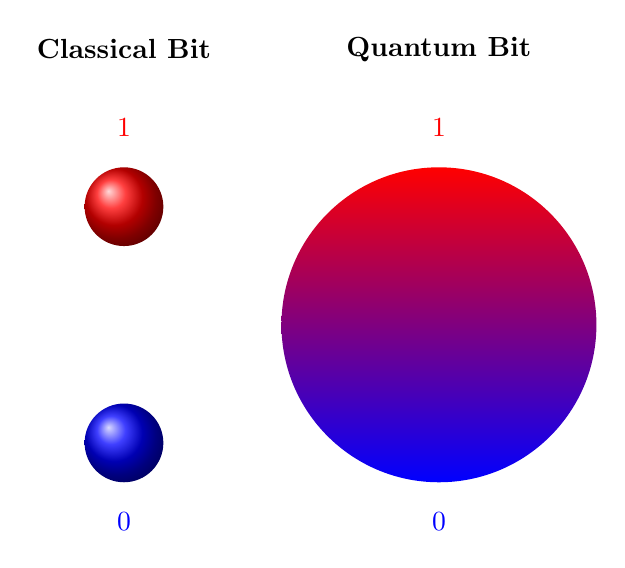
\begin{tikzpicture}[scale=1]
    \node[font=\bfseries] at (0,2) {Classical Bit};
    \node[font=\bfseries] at (4,2) {Quantum Bit};

    \node[color=red] at (0,1) {$1$};
    \node[color=blue] at (0,-4) {$0$};

    \node[shade,shading=ball,circle,ball color=blue,minimum size=1cm] (ball) at (0,-3) {};
    \node[shade,shading=ball,circle,ball color=red,minimum size=1cm] (ball) at (0,0) {};

    \node[color=red] at (4,1) {$1$};
    \node[color=blue] at (4,-4) {$0$};
    \node[shade, shading=ball,circle,top color=red, bottom color=blue, minimum size=4cm] (ball) at (4,-1.5) {};
  \end{tikzpicture}
  \caption{Conceptual illustration of the two-level classical bit, which are restricted to the boolean states 1 (true) or 0 (false), and the quantum bit that can be in any superposition of the states 0 or 1.}
  \label{fig:qubit and bit}
\end{wrapfigure}


It has been demonstrated that exponentially complex problems can be reduced to polynomially complex problems for quantum computers \cite{Pavicic2006}. For example, a quantum search algorithm found by Grover \cite{Grover1997} offers a quadratic speed-up compared to classical algorithms, while Shor's quantum integer factorization algorithm \cite{Shor1994} presents an exponential speed-up. Intriguingly, Google reported in $2019$ that they ran a random number generator algorithm on a superconducting processor containing 53 qubits in $200$ seconds, which would most likely take several times longer for a classical supercomputer to solve \cite{Martinis2019}. It is anticipated that quantum computers will excel in exceedingly complex problems, while many simpler tasks may not see any speed-up at all compared to the classical regime. Hence, quantum- and classical computers are envisioned to coexist to utilize the strength of each technology.

%However, it is not to avoid that both quantum  hardware and -software is in its preliminary phase of development, and it will be interesting to follow up the progression the following years.

Quantum computing is a highly sought-after goal, but there are extensive challenges that needs to be adressed. Controlling a complex many-qubit system is difficult, since it is not always possible to establish interactions between qubits \cite{DiVincenzo2000} and maintain entaglement over both time and distance. Additionally, decoherence and other quantum noise occurs as a result of the high volatility of quantum states, making quantum state manipulation prone to errors. The \textit{quantum error correction} protocols and the theory of \textit{threshold theorem} deals with this vulnerability, stating that noise most likely does not pose any fundamental barrier to the performance of large-scale computations \cite{Pavicic2006}.


\subsection{Quantum computing requirements}
As ever-promising the concepts of quantum technology are, the physical realizations are in the preliminary stage of development. Here we will concretize critical principles for a physical realisation of a quantum platform.

\begin{quote}
   ``I always said that in some sense, these criteria are exactly the ones that you would teach to kindergarten children about computers, quantum or otherwise'' DiVincenzo \cite{Georgescu2020}
\end{quote}

\noindent DiVincenzo formulated in the year of $2000$ seven basic criteria for a physical qubit system with a logic-based architecture \cite{DiVincenzo2000}.

\begin{enumerate}
  \item A scalable physical system with well characterized qubits
  \item The ability to initialize the state of the qubits to a simple initial system
  \item Have coherence times that are much longer than the gate operation time
  \item Have a universal set of quantum gates
  \item Have the ability to perform qubit-specific measurements
  %\item The ability to convert stationary qubits to flying qubits
  %\item The ability to faithfully transmit flying qubits between specified locations
\end{enumerate}

\noindent These five criteria must be met for a quantum platform to be considered a quantum computer.

%The first five criteria (1-5) must be met for a quantum platform to be considered a quantum computer, while the two last criteria (6-7) were added for quantum communication, since its applications provide a unique advantage compared to its classical counterpart.


%Quantum hardware and -software are both in the preliminary stage of development, and it will be interesting to follow their progress the following years.

\section{Quantum communication}

Quantum communication refers to the transfer of a state of one quantum system to another. Since information can be stored in qubits, we picture \textit{flying qubits} that transfer information from one location to another \cite{Griffiths2002}. The benefits of using flying qubits are in particular valued in quantum cryptography, since the quantum nature of qubits can be exploited to add extra layers of security \cite{Pavicic2006}.

%as it is regarding \textit{flying qubits} , a photon carrying a quantum state, which is an example of a \textit{flying qubit}.

%A significant portion of quantum communication is also part of other quantum information theories such as quantum cryptography, which comes as a remedy to a rising paranoia concerning security \cite{Griffiths2002, Pavicic2006}.

%Classical cryptography encrypts information with the use of a key.
Consider the example of encrypting a digitally transmitted conversation. It is difficult to avoid someone eavesdropping on a conversatio. However, the problem is diminished if the eavesdropper does not speak the language, keeping the information in the conversation safe. This is the original idea of encryption, such that the information has been encrypted into something incomprehensible for any eavesdropper. A common practice is to encrypt information and share a public key, which everyone can read, and a private key, only known for the sender and receiver of information. This should be sufficient to keep the information secure, given that the complexity of the private key is impenetrable.

Importantly, we live in a digital world where most of our actions are increasingly being stored as information, and we could imagine that the eavesdropper in the latter example stored the conversation. Even if the content of the conversation was encrypted, it still presents a challenge, since encrypted information stored today could be deciphered in ten or twenty years' time
%\footnote{As an example, in Martin Gardner's \textit{Scientific American} column in $1976$ \cite{Taubes1994}, the $129$-digit RSA key was thought to be safe for $5000$ mips (million instructions per second) years, equal to $4 \times 10^{25}$ years. Only $17$ years later, the factorization was a reality and the public key was revealed to be ``The Magic Words are Squeamish Ossifrage'' \cite{Atkins1995}. To compare to todays fastest supercomputer Fugaku \cite{Top500} by making two \textit{very} rough estimations that flops and mips are approximately the same in addition to solely basing the calculation on computing power, the $129$-digit RSA private key would be found in less than half a second using Fugaku.}
. Consequently, finding an encryption method that could make information either impossible to eavesdrop on or make the security unbreakable forever is very desirable. This is the ultimate goal of quantum cryptography \cite{Pavicic2006}.

Consider the example of information encoded into a qubit as a superposition of two quantum states. Now, if a wild eavesdropper would try to measure the information, the nature of quantum physics tells us that the original configuration would be destroyed and the receiver would be alerted of the eavesdropper. Furthermore, if the eavesdropper would try to make a copy of the message, the copying itself would be limited of the no-cloning theorem \cite{Gisin2002} which declare that quantum states cannot be copied.

A clever approach to ensure confidentiality is to send the encryption key before sending the actual encrypted information. If the key is received unperturbed, the key remains secret and can be safely employed. If it turns out perturbed, confidentiality is still intact since the key does not contain any information and can be discarded. This approach is termed the \textit{quantum key distribution} (QKD) \cite{Gisin2002, Gisin2007}. It should be noted that this requires both the sender and receiver to have access to methods for sending, receiving and storing qubit states, such as a quantum computer. Additionally, the sender and receiver will need to initially exchange a common secret which is later expanded, making quantum key \textit{expansion} a more exact term for QKD \cite{Pavicic2006, Gisin2007}.

Most applications and experiments use optical fibers for sending information via photons, with the distance regarded as the main limitation. This is because classical repeaters are unable to enhance quantum information because of the no-cloning theorem, making photon loss in optical fiber cables inevitable. Thus, quantum communication must reinvent the repeater concept, using hardware that preserves the quantum nature \cite{Acin2018} and are compatible with wavelengths used in telecommunication. Nonetheless, secure QKD up to $400$ km has recently been demonstrated using optical fibres in academic prototypes \cite{Boaron2018}.

\section{Quantum sensing}

Measurements are part of our digital world today to a great extent. There would be no way to exchange goods, services or information without reliable and precise measurements \cite{Acin2018}. Thus, improving the accuracy of sensors for all types of measurements is desirable. One potential method to improve measurement accuracy, resolution and sensitivity is utilizing quantum sensors. Quantum sensors exploit quantum properties to measure a physical quantity \cite{Degen2017}. This is possible because quantum systems are highly susceptible to pertubations to its surroundings, and can be used to detect physical properties such as either temperature or an electrical or magnetic field \cite{Degen2017}.

For a quantum system to be able to function as a quantum sensors, a few criterias needs to be met.  Firstly, the quantum system needs to have discrete and resolvable energy levels. The quantum system also needs to be controllably initialised into a state that can be identified and coherently manipulated by time-dependent fields. Lastly, the quantum system needs to be able to interact with the physical property one wants to measure through a coupling parameter \cite{Degen2017}.

It is also possible to also exploit quantum entanglement to improve the precision of a measurement. This gain of precision is used to reach what is called the Heisenberg-limit, which states that the precision scales as the number of particles $N$ in an idealized quantum system \cite{Degen2017, Acin2018}, while the best classical sensors scale with $\sqrt{N}$.

\section{Available quantum platforms}

%Before a quantum system can be used in either quantum computing, quantum cryptography or quantum sensing, a few criterias has to be met. They are formulated by

Many different quantum platforms have been physically implemented, and this section will serve as a brief overview of the current status. For a more thorough review of qubit implementations, the reader is directed to Refs. \cite{Ladd2010, Acin2018}. \\

Superconducting circuits can be used in quantum computing, since electrons in superconducting materials can form Cooper pairs via an effective electron-electron attraction when the temperature is lower than a critical limit. Below the limit, electrons can move without resistance in the material \cite{KristianFossheim2004}. Exploiting this intrinsic coherence, qubits can be made by forming microwave circuits based on loops of two superconducting elements separated by an insulator, also known as Josephson tunnel junctions \cite{Acin2018}. Today, superconducting Josephson junctions are the most widely used quantum platform, but they requires very low temperature (mK) to function, making them costly to use. Additionally, the current devices experience a relatively short coherence time, causing challenges in scaling up. \\

Single photons is an eligible quantum platform that can be implemented as qubits with one-qubit gates being formed by rotations of the photon polarization. Its use in fiber optics are less prone to decoherence, but faces challenges since the more complex photon-photon entanglement and control of multi-qubits is strenuous \cite{Ladd2010}. \\

By fixing the nuclear spin of solid-state systems, it is possible to implement a quantum platform that experience long spin coherence. This enables the manipulation of qubits that utilize electromagnetic fields, making one-qubit gates realizable. \\

The isolated atom platform is characterized by its well-defined atom isolation. Here, every qubit is based on energy levels of a trapped ion or atom. Quantum entanglement can be achieved through laser-induced spin coupling, however scaling up to large atom numbers induce problems in controlling large systems and cooling of the trapped atoms or ions. \\

A quantum dot (QD) can be imagined as an artifical atom which is confined in a solid-state host. As an example, a quantum dot can occur when a hole or an electron is trapped in the localized potential of a semiconductor's nanostructure. QDs exhibit similar coherence potential as the isolated atom platform, but without the drawback of confining and cooling of the given atom or ion \cite{Acin2018}. Moreover, it is possible to limit decoherence due to nuclear spins by dynamic decoupling of nuclear spin noise and isotope purification \cite{Ladd2010}.

A QD can normally be defined litographically using metallic gates, or as self-assembled QDs where a growth process creates the potential that traps electrons or holes. The difference between them is a question of controllability and temperature, since the metallic gates is primarily controlled electrically and operate at $<1$ K, while self-assembly QDs are primarily controlled optically at $\sim 4$ K \cite{Ladd2010}. Despite requiring very low temperatures, QDs have the potential for fast voltage control and opticial initialization. As with trapped ions, electrostatically defined quantum dots experience a short-range exchange interaction, imposing a limitation for quantum computing and quantum error correction protocols. A potential solution could include photonic connections between quantum dots. Indeed, self-assembled quantum dots couple strongly to photons due to their large size in comparison to single atoms. However, the size and shapes of self-assembled quantum dots are decided randomly during the growth process, causing an unfavourable large range of optical absorption and emission energies \cite{Ladd2010}.



%In such a system, the spin degree of freedom is considered favourable due to its long coherence time \cite{Acin2018}.

Lastly, we will turn towards point defects in bulk semiconductors as a physical implementation of a quantum platform. Point defects shares many of the attributes of quantum dots, such as discrete optical transitions and controllable coherent spin states. %but are vulnerable to small changes in the lattice of the semiconductor.
Depending on the semiconductor host and the defect system of interest, they may exhibit extended coherence times and greater optical homogeneity than other quantum dot systems. Before we dwell into the intricacies of point defect qubits as a building block for QT, we will provide the neccessary background for the crystal- and electronic structure of semiconductors.   %Thus, we will hereafter focus our attention on qubit host candidates.

\section{Introduction to semiconductor physics}

The interactions between atoms and the resulting characteristics of matter form the foundation of materials science. The applications of materials science are extensive, with examples such as a bottle of water or to a chair to sit in.

\begin{figure}[ht!]
  \centering
\begin{subfigure}{.5\linewidth}
\centering
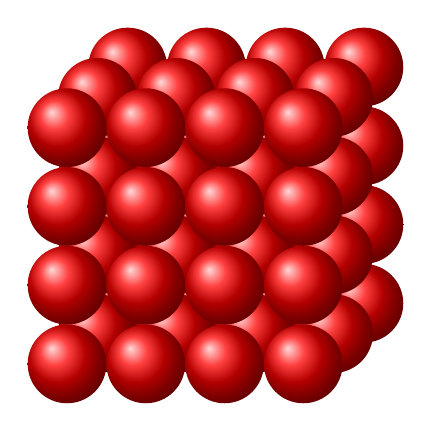
\begin{tikzpicture}
  \foreach \z in {1,2,3}{
  \foreach \i in {3,2,1,0}{% This one doesn't matter
    \foreach \j in {3,2,1,0}{% This will crate a membrane
        \shade[ball color=red] ({\i},{\j},\z) circle(0.5);
      }
    }
  }
\end{tikzpicture}
\subcaption{} \label{fig:M1}
\end{subfigure}%
\par\bigskip

\begin{subfigure}{1.0\linewidth}
\centering
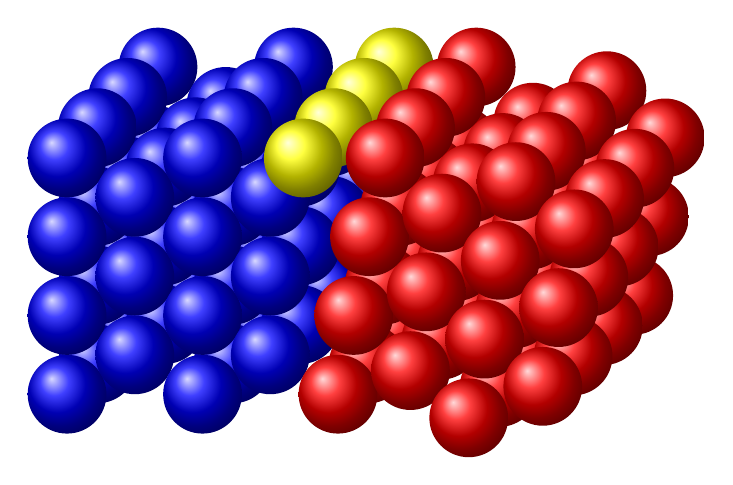
\begin{tikzpicture}
    \foreach \x in {0,1,2,3}{%
      \foreach \z in {0,1,2,3}{%
      \shade[ball color=blue] (0,\x,\z) circle(0.5);
      }
    }
    \foreach \x in {0.5,1.5,2.5}{%
      \foreach \z in {0,1,2,3}{%
      \shade[ball color=blue] ({1*sqrt(0.74)},\x,\z) circle(0.5);
      }
    }
    \foreach \x in {0,1,2,3}{%
      \foreach \z in {0,1,2,3}{%
      \shade[ball color=blue] ({2*sqrt(0.74)},\x,\z) circle(0.5);
      }
    }
    \foreach \x in {0.5,1.5,2.5}{%
      \foreach \z in {0,1,2,3}{%
      \shade[ball color=blue] ({3*sqrt(0.74)},\x,\z) circle(0.5);
      }
    }
    \foreach \z in {0,1,2,3}{%
      \shade[ball color=yellow] ({3},3,\z) circle(0.5);
    }
    \foreach \y in {0,1,2,3}{%
      \foreach \z in {0,1,2,3}{%
      \shade[ball color=red] ({4*sqrt(0.74)+0.2*\y},\y,\z) circle(0.5);
      }
    }
    \foreach \y in {0.3,1.3,2.3}{%
      \foreach \z in {0,1,2,3}{%
      \shade[ball color=red] ({5*sqrt(0.74)+0.2*\y},\y,\z) circle(0.5);
      }
    }
    \foreach \y in {-0.3,0.7,1.7,2.7}{%
      \foreach \z in {0,1,2,3}{%
      \shade[ball color=red] ({6*sqrt(0.74)+0.2*\y},\y,\z) circle(0.5);
      }
    }
    \foreach \y in {0.1,1.1,2.1}{%
      \foreach \z in {0,1,2,3}{%
      \shade[ball color=red] ({7*sqrt(0.74)+0.2*\y},\y,\z) circle(0.5);
      }
    }


\end{tikzpicture}
\subcaption{} \label{fig:M2}
\end{subfigure}%
\par\bigskip

\begin{subfigure}{1.0\linewidth}
\centering
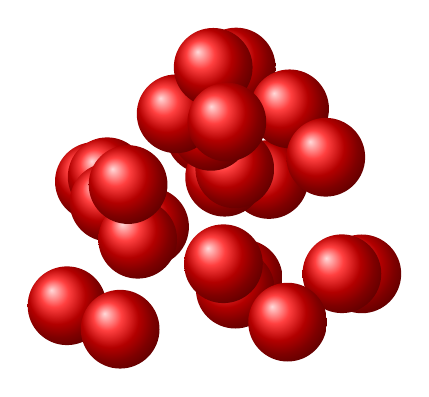
\begin{tikzpicture}
  \foreach \z in {0,...,24}{
    \shade[ball color=red] ({rand*1.5},{rand*1.5},{rand*1.5}) circle(0.5);
  }
\end{tikzpicture}
\subcaption{} \label{fig:M3}
\end{subfigure}
\par\bigskip
\caption{Schematic representation of different degrees of ordered structures, where (a) is a crystalline of a simple cubic lattice, (b) is a polycrystalline hexagonal lattice, and (c) is an amorphous lattice.}
\label{fig:crystalstructure}
\end{figure}


Solid materials, like plastic bottles, are formed by densely packed atoms. These atoms can randomly occur through the material without any long-range order or periodically ordered in small regions of the material, which would categorize the material as either an \textit{amorphous solid} or \textit{polycrystalline solid}. %, or the atoms can be periodically ordered in small regions of the materials,  %Amorphous solids are frequently used in gels, glass and polymers \cite{BenStreetman2015}.
%However, the atoms can also be periodically ordered in small regions of the material, classifying the material as a \textit{polycrystalline solid}.
%All ceramics are polycrystalline with a broad specter of applications ranging from kitchen-porcelain to orthopedical bio-implants \cite{Renganathan2018}.
A third option is to have these atoms arranged with infinite periodicity, making the material a \textit{crystalline solid} or more commonly named a \textit{crystal}. The three options are visualised in \autoref{fig:crystalstructure}. Hereon, we will focus on crystalline solids.

The periodicity in a crystal is defined in terms of a symmetric array of points in space called the \textit{lattice}, which can be simplified as either a one-dimensional array, a two-dimensional matrix or a three dimensional vector space, depending on the material. At each lattice point we can add an atom to make an arrangement called a \textit{basis}. The basis can be one atom or a cluster of atoms having the same spatial arrangement. Every crystal has periodically repeated building blocks called \textit{cells} representing the entire crystal. The smallest cell possible is called a \textit{primitive cell}, but such a cell only allows lattice points at its corners and it is often quite rigid to work with when the structure becomes complex. As a solution, we will consider the \textit{unit cell}, which allows lattice points on face centers and body centers.

One example of a crystal structure is the perovskite structure. Compounds with this structure are characterized by having an $ABX_3$ stoichiometry whose symmetri belong to one of 15 space groups identified by Lufaso \& Woodward \cite{Lufaso2001}, such as the cubic, orthorombic and tetragonal. For our purpose, we will be looking into when the X atom is oxygen, and refer to the oxygen-perovskite $ABO_3$. The A atom is nine- to 12-fold coordinated by oxygen, while the B atom is sixfold coordinated by oxygen, and the $BO_6$ octahedra are connected to the corners in all three directions as visualized in \autoref{fig:perovskite}.

\begin{wrapfigure}{r}{0.5\textwidth}
  \centering
  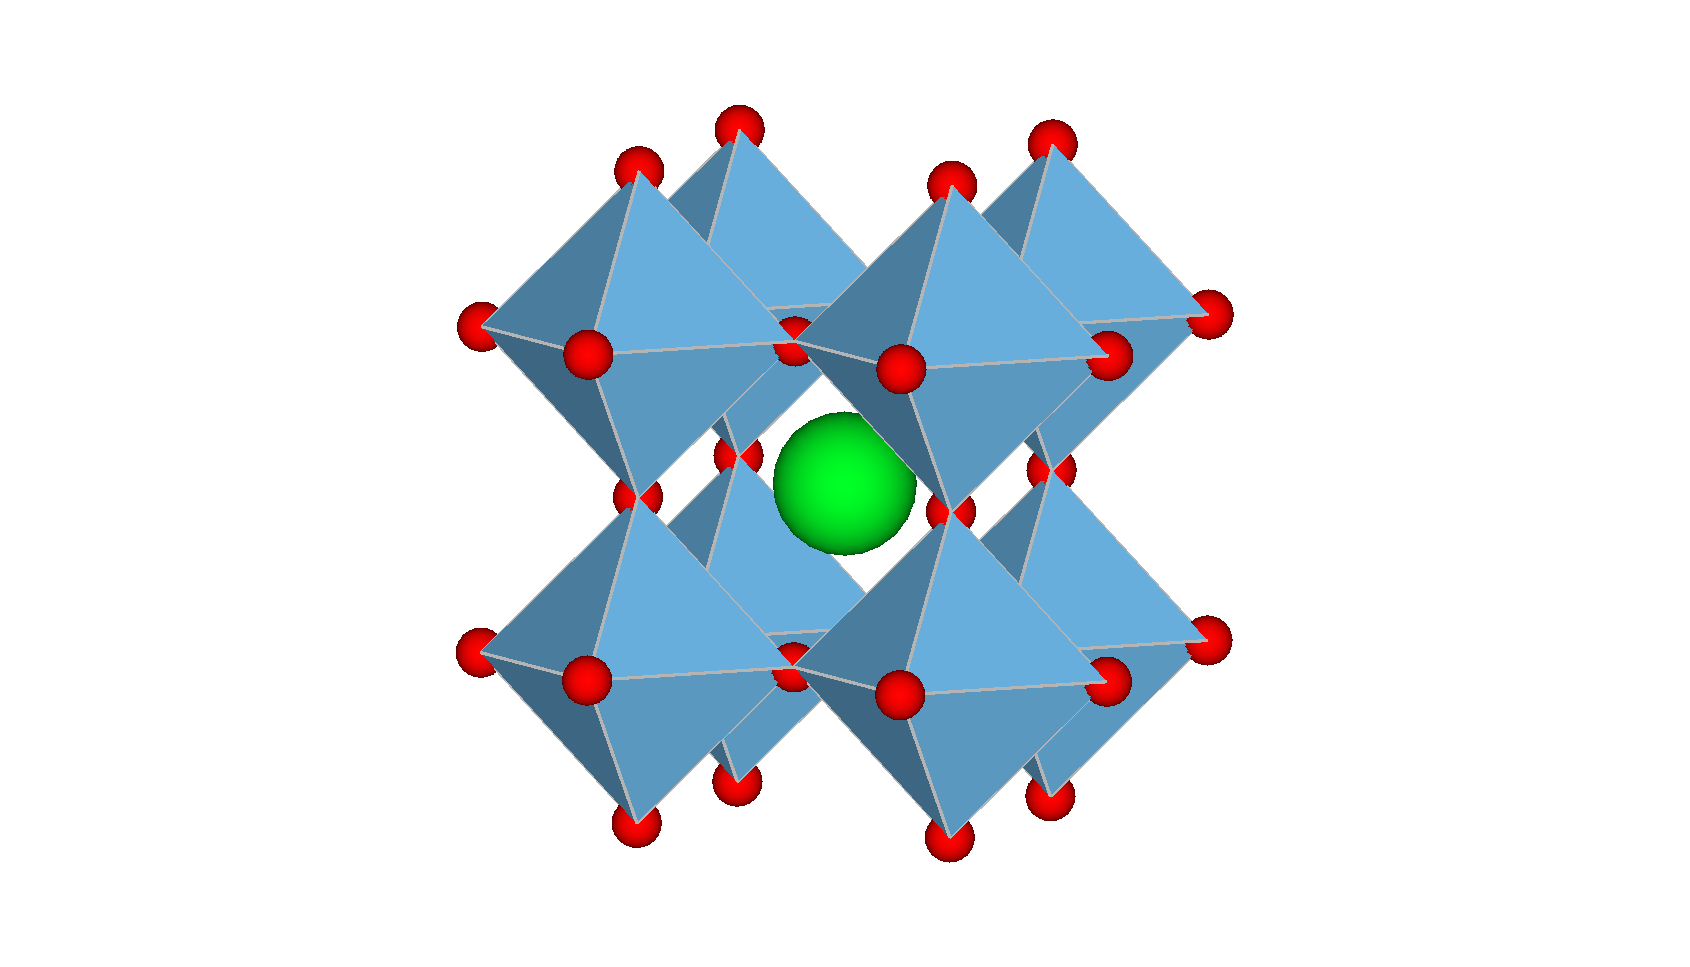
\includegraphics[width=0.48\textwidth]{theory/figures/SrTiO3_mp-5229_primitive.pdf}
  \caption{A crystal structure of SrTiO$_3$ which is a cubic perovskite. The red atoms are oxygen, whereas the green atom is strontium, and inside every corner-sharing BO$_6$ octahedral unit is a titanium atom.}
  \label{fig:perovskite}
\end{wrapfigure}

The motivation behind the research on perovskites is related to the large amount of available ABO$_3$ chemistries, where a significant portion of these take the perovskite structure. Perovskites have a broad specter of applications, ranging from high-temperature superconductors \cite{Bednorz1988} and ionic conductors \cite{Boivin1998} to multiferroic materials \cite{Cheong2007}. Additionally, adding a perovskite-type compound to solar cells has reportedly resulted in higher performance efficiencies while being cheap to produce and simple to manufacture \cite{IbnMohammed2017, Chen2014}. However, this includes the use of hybrid organic-inorganic compounds and excludes the use of oxygen.

%Point defects are the type of defect that can be utilised in generating a qubit, thus being a special interest for this thesis. They can arise as either a vacancy in the lattice, interstitial placement inbetween lattice sites, or as a substitution of an existing atom in the lattice.

%Her kan jeg skrive videre om NV -1 strukturen og defekten, da den blir brukt senere.


Isolated atoms have distinct energy levels, where the Pauli exlusion principle \cite{Pauli1925} states for fermions that each energy level can at most accomodate two electrons of opposite spin. In a solid, the discrete energy levels of the isolated atom spread into continuous energy bands since the wavefunctions of the electrons in the neighboring atoms overlap. Hence, an electron is not neccessarily localized at a particular atom anymore. This is exemplified as every material has a unique band structure, similar to every human having their unique fingerprint.

Knowing which energy bands are occupied by electrons is the key in understanding the electrical properties of solids. The highest occupied electron band at $0$ K is called the valence band (VB), while the lowest unoccupied electron band is called the conduction band (CB). The energy gap between the maximum VB and the minimum CB is known as the band gap, and its energy is denoted as $E_g$. If a material can be classified as a semiconductor depends on the band gap and the electrical conductivity. As an example, Silicon is commonly thought of as a semiconductor, and has a band gap of about $1.12$ eV at $275$ K \cite{Martienssen2005}.


\begin{wrapfigure}{r}{0.35\textwidth}
  \begin{minipage}{\linewidth}
    \centering\captionsetup[subfigure]{justification=centering}
  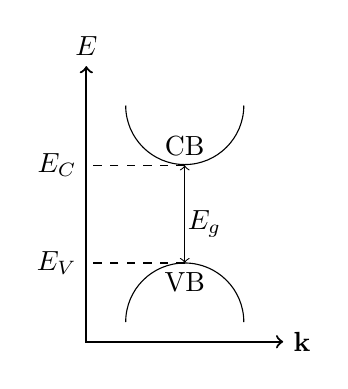
\begin{tikzpicture}[scale=1]
      \draw [<->,thick] (0,3.5) node (yaxis) [above] {$E$}
          |- (2.5,0) node (xaxis) [right] {$\textbf{k}$};
      \draw (0.5,0.25) arc(180:0:0.75cm);
      \draw (2.0,3.0) arc(0:-180:0.75cm);
      \coordinate (VB) at (1.25,1.0);
      \coordinate (CB) at (1.25,2.24);
      \draw[<->] (CB) node[above] {CB}
        -| (VB) node[below] {VB};
      \draw[dashed] (VB) -- (0,1.0) node[left]{$E_V$};
      \draw[dashed] (CB) -- (0,2.24) node[left]{$E_C$};
      \node at (1.5,1.5) {$E_g$};
  \end{tikzpicture}
  \subcaption{}
  \label{fig:directbandgap}
  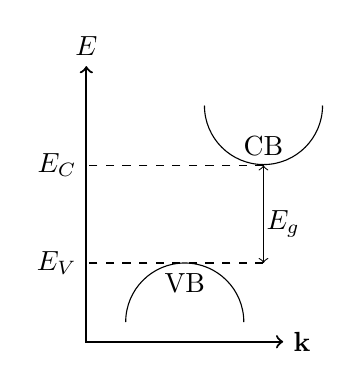
\begin{tikzpicture}[scale=1]
      \draw [<->,thick] (0,3.5) node (yaxis) [above] {$E$}
          |- (2.5,0) node (xaxis) [right] {$\textbf{k}$};
      \draw (0.5,0.25) arc(180:0:0.75cm);
      \draw (3.0,3.0) arc(0:-180:0.75cm);
      \coordinate (VB) at (2.25,1.0);
      \coordinate (CB) at (2.25,2.24);
      \draw[<->] (CB) node[above] {CB}
        -| (VB);
      \draw[dashed] (VB) -- (0,1.0) node[left]{$E_V$};
      \draw[dashed] (CB) -- (0,2.24) node[left]{$E_C$};
      \node at (2.5,1.5) {$E_g$};
      \node at (1.25,0.75) {VB};
  \end{tikzpicture}
  \label{fig:indirectbandgap}
  \subcaption{}
  \end{minipage}
  \caption{A schematic drawing of a (a) direct bandgap and an (b) indirect bandgap.}
\end{wrapfigure}


To be able to accelerate electrons in a solid using an electrical field, they must be able to move into new energy states. At $0$ K, the entire valence band of a semiconductor is full with electrons and there are no available states nearby, making it impossible for current to flow through the material. This can be solved by using either thermal or optical energy to excite electrons from the valence band to the conduction band, in order to \textit{conduct} electricity. At a given temperatuer, some semiconductors will have electrons excited to the conduction band solely from thermal energy matching the energy band gap \cite{BenStreetman2015}.

In some scenarios, thermal or optical energy is not sufficient for an excitation since the energy bands are also dependent on the crystal momentum. A difference in the momentum of the minimal-energy state in the conduction band and the maximum-energy state in the valence band results in an \textit{indirect bandgap} as seen in figure \autoref{fig:indirectbandgap}. If there is no difference at all, the material has a \textit{direct bandgap}, which is visualized in \autoref{fig:directbandgap}.

Electrons in semiconductor materials can be described according to the Fermi-Dirac distribution
\begin{align*}
  f(E) = \frac{1}{1+e^{(E-E_F)/kT}},
\end{align*}
where $k$ is Boltzmann's constant, $T$ is temperature, $E$ is the energy and $E_F$ is the Fermi level. The Fermi-Dirac distribution gives the probability that a state will be occupied by an electron, and at $T=0$ K, every energy state lower than $E_F$ is occupied by electrons while the opposite is true for energy states above $E_F$ \cite{BenStreetman2015}.

\subsection{Point defects in semiconductors}

In real life, a perfect crystal without any symmetry-breaking flaw does not exist. These flaws are known as defects and can occur up to three dimensions. An example one-dimensional defect is known as a \textit{line defect}, while two dimensional defects can be \textit{planar defects}, and in three dimensions we have \textit{volume defects}. Lastly, defects can also occur in zero dimensions and are then termed \textit{point defects}. Point defects normally occur as either vacancies, interstitially placed atoms inbetween lattice sites (called interstitials) or as substitution of another existing atom in the lattice.

Defects can greatly influence both the electronic and optical propertires of a material. A substitional defect may be an unintentionally introduced impurity or an antisite, but they can also be intentionally inserted, an approach normally known as \textit{doping}. Doping can result in an excess of electrons or holes, making the semiconductor either an n- or p-type, respectively. Consequently, the semiconductor will have energy levels in the (forbidden) band gap that originates from the defects. If the energy levels introduced are closer than $ \sim 0.2$ eV to the band egdes, they are termed \textit{shallow} defects.

Shallow defects can contribute with either excess electrons to the conduction band, or excess holes to the valence band. However, the induced charge carriers (electrons or holes) interact strongly with the band egdes, resulting in a delocalized wavefunction.% regarding the position in the lattice. %For the latter scenario, shallow defects are commonly labelled as \textit{dopants}.

For the opposite case, if the energy levels rests closer to the middle of the semiconductor's gap, the introduced defects are known as \textit{deep level} defects. Deep levels may be of intrinsic or extrinsic origin, %normally occur due to either dangling bonds or impurities,
and have highly localized electron wavefunctions. This might assure the isolation required for long coherence times, which is an appealing promise in quantum technological advances.

Deep levels can be unfortunate in semiconductors since they can interact with the charge carriers, potentially modifying the desired electronic or optical property of the material. Deep level defects can function as electron-hole recombination centers, or to trap charge carriers, yielding the commonly used name deep level \textit{traps}. Both of the given situations results in a lower concentration of charge carriers, which showcase why deep levels normally are unwanted in semiconductor devices. However, deep level defects may be beneficially used in quantum technology. %show extraordinary properties in quantum technology due to their ability to ensure isolation and preserve coherence.

\subsection{Optical defect transitions}

Optical transitions refers to excitation or de-excitation of charge carriers due to either emission or absorption of electromagnetic radiation.%, and can be done with a laser light or electron beam.
\autoref{fig:configurationcoordinate} represents a configuration coordinate (CC) diagram of a defect transition. The y-axis is the energy $E$, while the x-axis is the configuration coordination $Q$, which represents the atomic displacement from the equilibrium position $Q_{GS}$. The lowest point in the lower parabola is known as the ground state (GS) configuration $Q_{GS}$, which is the most stable atomic position, while for the upper parabola it is known as the excited state configuration $Q_{ES}$. The dotted lines represent vibronic excitations to the energy of the ground state $Q_{GS}$ for the lower parabola, while it represents $Q_{ES}$ for the higher parabola.


\begin{figure}[!ht]
  \centering
  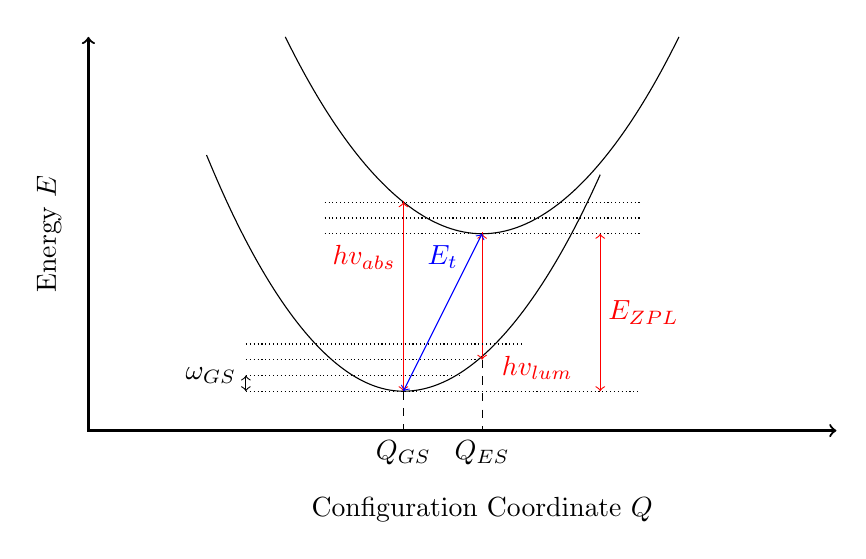
\begin{tikzpicture}[scale=1]
      \draw [<->,thick] (0,5.0) node (yaxis) [left] {}
          |- (9.5,0) node (xaxis) [below left] {};

      \draw (1.5,3.5) parabola bend (4,0.5) (6.5,3.25);
      \draw (2.5,5.0) parabola bend (5.0,2.5) (7.5,5.0);
      \node[rotate=90] at (-0.5,2.5){\text{Energy} $E$};

      \draw[<->, color=red] (4.0,2.9)
        -| (4.0,0.50);

      \draw[<->, color=red] (5.0,2.5)
          -| (5.0,0.9);

      \draw[<->, color=blue] (4.0,0.50) -- (5.0,2.5);
      \node[color=red] at (3.5,2.2) {$hv_{\text{abs}}$};
      \node[color=blue] at (4.5,2.2) {$E_t$};
      \node[color=red] at (5.7,0.8) {$hv_{\text{lum}}$};

      \draw[densely dotted] (2.0,0.5) -- (7.0,0.5);
      \draw[densely dotted] (2.0,0.7) -- (4.75,0.7);
      \draw[densely dotted] (2.0,0.9) -- (5.0,0.9);
      \draw[densely dotted] (2.0,1.1) -- (5.5,1.1);

      \draw[<->] (2.0,0.50) -- (2.0,0.7) node[left]{$\hslash \omega_{GS}$};

      \draw[densely dotted] (3.0,2.5) -- (7.0,2.5);
      \draw[densely dotted] (3.0,2.7) -- (7.0,2.7);
      \draw[densely dotted] (3.0,2.9) -- (7.0,2.9);

      \draw[<->, color=red] (6.5,0.50) -- (6.5,2.5);
      \node[color=red] at (7.05,1.5) {$E_{ZPL}$};

      \draw[dashed] (4.0,0.50) -- (4.0,0.0) node[below]{$Q_{GS}$};
      \draw[dashed] (5.0,0.9) -- (5.0, 0) node[below]{$Q_{ES}$};

      \node at (5.0,-1.0){\text{Configuration Coordinate} $Q$};
      %\draw[dashed] (VB) -- (0,1.0) node[left]{$E_V$};
      %\draw[dashed] (CB) -- (0,2.24) node[left]{$E_C$};
      %\node at (2.5,1.5) {$E_g$};
      %\node at (1.25,0.75) {VB};
  \end{tikzpicture}
  \caption{A schematic representation of a configuration coordination diagram based on Ref. \cite{Pelant2012}.}
  \label{fig:configurationcoordinate}
\end{figure}


\noindent The optical transitions in \autoref{fig:configurationcoordinate} are marked with red arrows. During slow transitions, such as during thermodynamic defect transitions, the original configuration have time to rearrange due to phonon vibrations. This is schematically drawn as the blue arrow, where the energy $E_t$ equals the ionization energy or the position of the defect level. Optical transitions, on the other hand, are marked in red and occur in a short time range such that the original configuration does not change. They can appear in the exchange of charge carriers with the band egdes, and in a defect's internal excited state, with the latter scenario being most relevant for this thesis.

Consider a defect that rests in the ground state configuration $Q_{GS}$. Suddenly, it absorbs a photon with energy $h v_{\text{abs}}$ and occupies an excited vibronic state of the upper parabola after a vertical transition. Through lattice reconfigurations, the defect will move towards the bottom of the upper parabola, also known as $Q_{ES}$. Eventually, it will relax to the lower parabola by emitting a photon with energy $h v_{lum}$, also known as a zero-phonon line (ZPL) of energy $E_{ZPL}$. On the other hand, any transitions between vibronic excitation levels are phonon-related. How strong the electron-phonon interaction is can be quantified by the Huang-Rhys factor $S$ \cite{Huang1950}. If the two parabolas in \autoref{fig:configurationcoordinate} have the same configuration of $Q$, emission into the ZPL is enabled and $S\sim 0$. The stronger the coupling, the smaller amount of emission in the ZPL.

The optical properties of a host material can be greatly influenced by defects, in particular the ES to GS transition that can occur in a defect, as discussed for \autoref{fig:configurationcoordinate}. If the defect were to fascilitate the emission of single photons with a detectable time inbetween together with a distinguishable ZPL, the defect would be referred to as a single photon source (SPS). The criteria for SPS are not met in many materials or defect systems, since charge-state transitions often comprise interactions with either the VB or the CB. Thus, most SPSs' GS and ES levels are situated within the band gap of a host material. Consequently, mostly wide-band gap semiconductors are used as host materials for SPSs.

\section{Semiconductor candidates for quantum technology}

The properties of point defects are promising in a quantum technological perspective. We have seen that point defects can fasciliate deep energy levels within the band gap of the semiconductor, and provide isolation in the solid-state matrix as a result from a high degree of localization of the defect orbitals. If the host material have a small spin-orbit coupling, it could provide long coherence times for a deep level trap in localized and high-spin states. Additionally, point defects have the potential to be single-photon sources, giving rise to sharp and distinguishable optical transitions, where a significant amount of the emission can be of the energy $E_{ZPL}$. This is in particular seen in wide-bandgap semiconductors, and combined with a weak electron-phonon interaction, can have the capacity to be fabricated as a high-fidelity SPS with a significant ZPL part.

In this section we will provide specific examples of a variety of promising candidates, and what properties they possess that makes them auspicious. Additionally, we will briefly mention what the challenges with the candidates are, and why it is important to explore other viable options.

\subsection{Diamond - the benchmark material for QT}
\label{diamond}

\begin{figure}[ht!]
  \centering
\begin{subfigure}{1.0\linewidth}
\centering
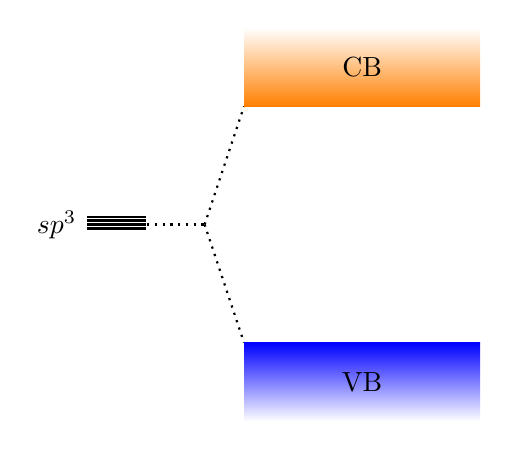
\begin{tikzpicture}

  \atom[name=C, color=orange, pos={(-2,0)},scale=0.5]{
    gray/45/45/0,
    gray/315/315/0,
    gray/225/225/0,
    gray/135/135/0}

  \draw[thick,-] (-1.25,-4) -- (-2.0,-4) node[anchor=east]{$sp^3$};
  \draw[thick,-] (-1.25,-3.95) -- (-2.0,-3.95);
  \draw[thick,-] (-1.25,-4.05) -- (-2.0,-4.05);
  \draw[thick,-] (-1.25,-3.90) -- (-2.0,-3.90);

  \draw[thick, dotted] (-1.23,-4) -- (-0.5,-4);
  \draw[thick, dotted] (-0.5,-4) -- (0,-5.5);
  \draw[thick, dotted] (-0.5,-4) -- (0,-2.5);

  %\node at (1.5,1.5) {$E_g$};
  %\draw (0,-1.5) -- (2,-1.5) -- (2,-2) -- (0,-2) -- (0,0);
  \shade[top color=white,bottom color=orange] (0,-2.5) rectangle (3.0,-1.5) node[pos=.5] {CB};
  \shade[top color=blue,bottom color=white] (0.,-6.5) rectangle (3.0,-5.5) node[pos=.5] {VB};

  \atom[name=C, color=orange, scale=0.5]{
    gray/45/45/0,
    gray/315/315/0,
    gray/225/225/0,
    gray/135/135/0}
  \atom[name=C, color=orange, pos={(0.75,0.75)},scale=0.5]{
    gray/45/45/0,
    gray/315/315/0,
    gray/225/225/0,
    gray/135/135/0}
  \atom[name=C, color=orange, pos={(1.5,0)},scale=0.5]{
    gray/45/45/0,
    gray/315/315/0,
    gray/225/225/0,
    gray/135/135/0}
  \atom[name=C, color=orange, pos={(0.75,-0.75)},scale=0.5]{
    gray/45/45/0,
    gray/315/315/0,
    gray/225/225/0,
    gray/135/135/0}
  \atom[name=C, color=orange, pos={(2.25,0.75)},scale=0.5]{
    gray/45/45/0,
    gray/315/315/0,
    gray/225/225/0,
    gray/135/135/0}
  \atom[name=C, color=orange, pos={(2.25,-0.75)},scale=0.5]{
    gray/45/45/0,
    gray/315/315/0,
    gray/225/225/0,
    gray/135/135/0}
  \atom[name=C, color=orange, pos={(3.0,0)},scale=0.5]{
      gray/45/45/0,
      gray/315/315/0,
      gray/225/225/0,
      gray/135/135/0}

\end{tikzpicture}
\subcaption{} \label{fig:diamond structure}
\end{subfigure}%

\begin{subfigure}{1.0\linewidth}
\centering
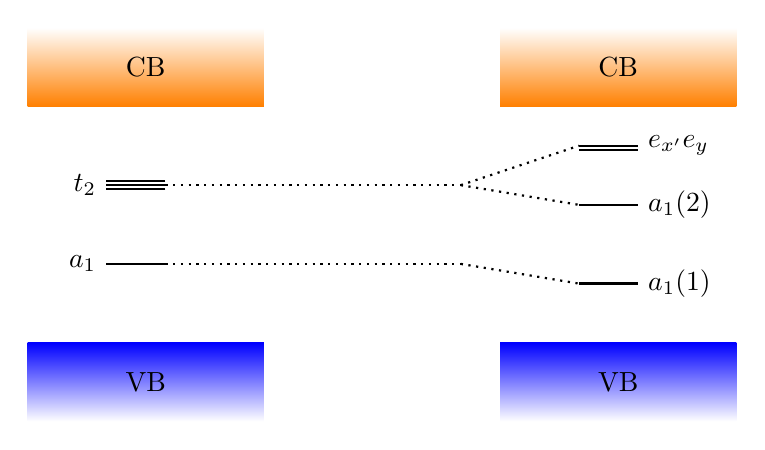
\begin{tikzpicture}

  \shade[top color=white,bottom color=orange] (0.-7,-2.5) rectangle (3.0-7,-1.5) node[pos=.5] {CB};
  \shade[top color=blue,bottom color=white] (0.-7,-6.5) rectangle (3.0-7,-5.5) node[pos=.5] {VB};

  \draw[thick,-] (1.75-7,-4.5) -- (1.0-7,-4.5) node[anchor=east]{$a_1$};
  \draw[thick,-] (1.75-7,-3.5) -- (1.0-7,-3.5) node[anchor=east]{$t_2$};
  \draw[thick,-] (1.75-7,-3.55) -- (1.0-7,-3.55);
  \draw[thick,-] (1.75-7,-3.45) -- (1.0-7,-3.45);

  \atom[name=C, color=orange, pos={(0-7,0)}, scale=0.5]{
    gray/45/45/0,
    gray/315/315/0,
    gray/225/225/0,
    gray/135/135/0}
  \atom[name=C, color=orange, pos={(0.75-7,0.75)},scale=0.5]{
    gray/45/45/0,
    red/315/315/0,
    gray/225/225/0,
    gray/135/135/0}
  \atom[name=v, color=gray, pos={(1.5-7,0)},scale=0.5]{}
  \atom[name=C, color=orange, pos={(0.75-7,-0.75)},scale=0.5]{
    red/45/45/0,
    gray/315/315/0,
    gray/225/225/0,
    gray/135/135/0}
  \atom[name=C, color=orange, pos={(2.25-7,0.75)},scale=0.5]{
    gray/45/45/0,
    gray/315/315/0,
    red/225/225/0,
    gray/135/135/0}
  \atom[name=C, color=orange, pos={(2.25-7,-0.75)},scale=0.5]{
    gray/45/45/0,
    gray/315/315/0,
    gray/225/225/0,
    red/135/135/0}
  \atom[name=C, color=orange, pos={(3.0-7,0)},scale=0.5]{
      gray/45/45/0,
      gray/315/315/0,
      gray/225/225/0,
      gray/135/135/0}

    \shade[top color=white,bottom color=orange] (0.-1.,-2.5) rectangle (3.0-1.0,-1.5) node[pos=.5] {CB};
    \shade[top color=blue,bottom color=white] (0.-1.,-6.5) rectangle (3.0-1.0,-5.5) node[pos=.5] {VB};

    \atom[name=C, color=orange, pos={(0.-1.,0)}, scale=0.5]{
      gray/45/45/0,
      blue/315/315/0,
      gray/225/225/0,
      gray/135/135/0}
    \atom[name=C, color=orange, pos={(0.75-1,0.75)},scale=0.5]{
      gray/45/45/0,
      red/315/315/0,
      gray/225/225/0,
      gray/135/135/0}
    \atom[name=v, color=gray, pos={(1.5-1,0)},scale=0.5]{}
    \atom[name=N, color=green!95, pos={(0.75-1,-0.75)},scale=0.5]{
      blue/45/45/0,
      blue/315/315/0,
      blue/225/225/0,
      blue/135/135/0}
    \atom[name=C, color=orange, pos={(2.25-1,0.75)},scale=0.5]{
      gray/45/45/0,
      gray/315/315/0,
      red/225/225/0,
      gray/135/135/0}
    \atom[name=C, color=orange, pos={(2.25-1,-0.75)},scale=0.5]{
      gray/45/45/0,
      gray/315/315/0,
      gray/225/225/0,
      red/135/135/0}
    \atom[name=C, color=orange, pos={(3.0-1,0)},scale=0.5]{
        gray/45/45/0,
        gray/315/315/0,
        gray/225/225/0,
        gray/135/135/0}

    \draw[thick, dotted] (1.75-7,-3.5) -- (-1.5,-3.5);
    \draw[thick, dotted] (-1.5,-3.5) -- (0,-3.0);
    \draw[thick, dotted] (-1.5,-3.5) -- (0,-3.75);

    \draw[thick,-] (1.0-1,-3.0) -- (1.75-1,-3.0) node[anchor=west]{$e_{x'}e_y$};
        \draw[thick,-] (1.75-1,-3.05) -- (1.0-1,-3.05);
    \draw[thick,-] (1.0-1,-3.75) -- (1.75-1,-3.75) node[anchor=west]{$a_1(2)$};

    \draw[thick, dotted] (1.75-7,-4.5) -- (-1.5,-4.5);
    \draw[thick, dotted] (-1.5,-4.5) -- (0,-4.75);
    \draw[thick,-] (1.0-1,-4.75) -- (1.75-1,-4.75) node[anchor=west]{$a_1(1)$};

\end{tikzpicture}
\subcaption{} \label{fig:defect diamond structure}
\end{subfigure}
\par\bigskip
\caption{A schematic representation of the electronic structure of the NV$^{-1}$ defect in a tetrahedrally coordinated semiconductor, exemplified by diamond. Figure used from Ref. \cite{Gordon2013}.}
\label{fig: diamond electronic structure}
\end{figure}


The most studied point defect system is the nitrogen-vacancy ($NV^{-1}$) in diamond. \autoref{fig: diamond electronic structure} schematically shows the negative charge state of the electronic structure in diamond. Panel \autoref{fig:diamond structure} shows the electronic states that correspond to the difference for an isolated atom and a lattice of atoms, as a superposition of $sp^3$ orbitals that generates valence and conduction bands. In panel \autoref{fig:defect diamond structure}, a vacancy has been created by removing a carbon atom, and the four orbitals interact with each other resulting in two new states with $a_1$ and $t_2$ symmetry due to dangling bonds. Substituting a carbon atom with a nitrogen atom further splits the $t_2$-states into two new states. The states $a(1)$ and $e_{x'}e_y$ are of importance, as they are the GS and the ES of the qubit defects, respectively. Here, an optical spin-conserving transition can occur due to a laser light of correct wavelength \cite{Gordon2013}, as exemplified from the discussion from the last section.

\noindent The nitrogen-vacancy in diamond is a prominent single-photon source up to room temperatures. This involves initializing, manipulating and reading out of the qubit state using optical and electric excitations, and electric and magnetic fields \cite{Gordon2013}. The potential qubit system have promising applications in quantum- communication and computation, with a demonstrated entanglement between two NV center spins that are separated by $3$ m \cite{Bernien2013}. Nevertheless, perhaps the most propitious application can be seen in quantum sensing as high-sensivity magnetometer with nanoscale resolution \cite{Taylor2008}.

Unfortunately, the NV-center display several drawbacks that may limit the use in quantum communication and computation. In particular, the amount of emission into the zero-phonon line is only $4 \%$ at $6$ K \cite{Barclay2011}. The emission of the qubit center is not completely compatible with current optical fiber technologies, since the emission is in the red wave-length specter. Additionally, fabricating materials of diamond is far from unchallenging and serves as a signficant incentive to find other promising qubit candidates.

\subsection{Qubit material host requirements}
\label{ssec:qubit-material-host-requirements}
Therefore, we turn to the search of other QT compatible hosts that offers similar capabilities, but that are more user-friendly. In particular, we need to search for new promising materials that can host a potential point defect. \citeauthor{Weber2010} \cite{Weber2010} proposed in 2010 four criteria that should be met for a solid-state semiconductor material hosting a qubit defect, whereas some of the criteria has already been discussed. An ideal crystalline host should have \cite{Weber2010}
\begin{itemize}
  \item[(H1)] A wide-band gap to accomodate a deep center.
  \item[(H2)] Small spin-orbit coupling in order to avoid unwanted spin flips in the defect bound states.
  \item[(H3)] Availability as high-quality, bulk, or thin-film single crystals.
  \item[(H4)] Constituent elements with naturally occuring isotopes of zero nuclear spin.
\end{itemize}

%Host candidates that satisfy criteria (H1) and (H2) can be found by studying the electronic structure of the compounds. What tends to happen for defects in semiconductors, is that the electronic states associated with the defect have energies that lie within the (forbidden) band gap of the semiconductor. This is schematically drawn and explained for diamond in figure (\autoref{fig: diamond electronic structure}). A large band gap can accomodate multiple highly isolated states and make them confined and isolated from interactions with the environment, which is favorable for longer coherence times. However, the desired band gap depends on the application, since the Fermi level of large band gap materials is challenging to control \cite{Bassett2019}.

\noindent Table (\autoref{tab:qubithosts}) lists several material host candidates that exhibit promising band gap capable of accommodating a deep level defect. For example, the spin-orbit splitting is an indication of the strength of the spin-orbit interaction, and is taken at the $\Gamma$ point from the valence-band splitting. A smaller value may indicate less susceptibility to decoherence.

\begin{table}[!ht]
\centering
\noindent\makebox[\textwidth]{
\begin{tabular}{M{2.5cm} M{2.5cm} M{3.0cm} M{4.0cm}}
  \hline
  \hline
  Material & Band gap  $E_g$ (eV) & Spin-orbit splitting $\Delta_{so}$ (meV) & Stable spinless nuclear isotopes? \\
  \hline
  3C-SiC & 2.39 & 10 & Yes \\
  4H-SiC & 3.26 \cite{Neudeck1995} & 6.8 & Yes \\
  6H-SiC & 3.02 & 7.1 & Yes \\
  AlN & 6.13 & 19 \cite{Silveira2005} & No \\
  GaN & 3.44 & 17.0 & No \\
  AlP & 2.45 & 50 \cite{Lawaetz1971} & No \\
  GaP & 2.27 & 80 & No \\
  AlAs & 2.15 & 275 & No \\
  ZnO & 3.44 \cite{Beckers1998} & -3.5 & Yes \\
  ZnS & 3.72 \cite{Kumbhojkar2000} & 64 & Yes \\
  ZnSe & 2.82 & 420 & Yes \\
  ZnTe & 2.25 & 970 & Yes \\
  CdS & 2.48 & 67 & Yes \\
  \hline
  C (Diamond) & 5.5 & 6 & Yes \\
  Si & 1.12 & 44 & Yes \\
  \hline
  \hline
\end{tabular}
}
\caption{Table taken from \citeauthor{Gordon2013} \cite{Gordon2013} that lists a number of tetrahedrally coordinated hosts whose band gaps are larger than $2.0$ (eV), and compares it to diamond and Si. All experimental values are from Ref. \cite{Martienssen2005}, except for where explicity cited otherwise. }
%For materials where more than one structure is stable in room temperature, the most dominant room-temperature phase's band parameters are chosen.}
\label{tab:qubithosts}
\end{table}

Criterion (H3) is important for scalability and further potential for a large-scale fabrication. The given candidate hosts provided in table (\autoref{tab:qubithosts}) can all be grown as single crystals, but with varying quality and size.

\noindent Normally, nuclear spin is a major source of decoherence for all semiconductor-based quantum technologies. This would exclude the use of all elements in odd groups in the periodic table, since these elements exhibit nonzero nuclear spin. As a result, the spin-coherence time of a paramagnetic deep center \cite{Weber2010} might increase. However, nuclear spin can also induce additional quantum degrees of freedom for applications in the proper configuration \cite{Bassett2019}. Therefore, criterion (H4) is not a strict requirement but is a general recommendation for reducing decoherence time.  %Therefore, we will not completely exclude all nonzero nuclear spin elements from our list.

%In fact, all of the criteria could be regarded as recommendations,

\citeauthor{Weber2010} \cite{Weber2010} use criteria $(H1)-(H4)$ to specifically find analogies to the $NV^{-1}$ center in other material systems, thus leaving the discussion of other criteria out, such as the choice of crystal system. The atomic configuration and crystal structure of a material strongly influences the properties of a defect, since a defect's orbital and spin structure is dependent on its spatial symmetry \cite{Bassett2019}. In particular, it is the point group that decides which multiplicity a given energy level should have \cite{James1976}. A higher defect symmetry group generally facilitates degenerate states, which may give rise to high spin states according to Hund's rules \cite{Bassett2019, Togan2010}. Inversion symmetry in the host crystal can also be beneficial, resulting in reduced inhomogenous broadening and spectral diffusion of optical transitions as a consequence of being generally insensitive to external electric fields \cite{Bassett2019}.

\begin{wrapfigure}{r}{0.6\textwidth}
  \centering
  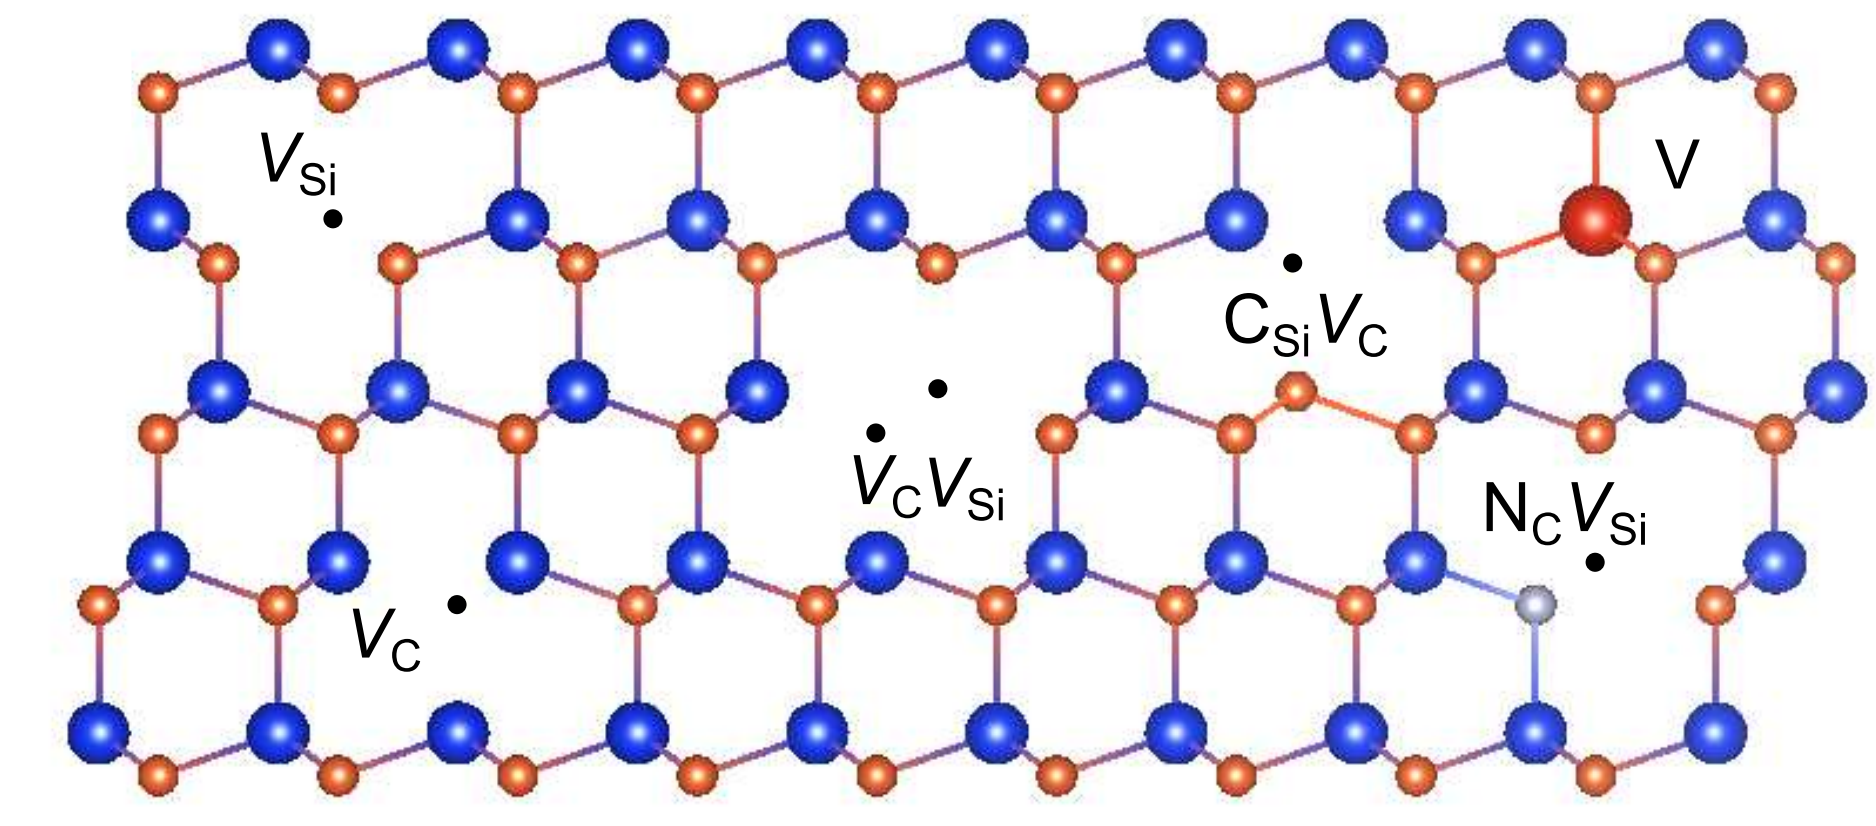
\includegraphics[width=0.6\textwidth]{theory/figures/4H-SiC.png}
  \caption{Schematic illustration of various point defects in 4H-SiC, where Si atoms are blue while C atoms are orange. The illustration includes the point defects Si vacancy ($\text{V}_{\text{Si}}$), C vacancy ($\text{V}_{\text{C}}$), divacancy ($\text{V}_{\text{Si}}\text{V}_{\text{C}}$), carbon antisite-vacancy pair ($\text{C}_{\text{Si}}\text{V}_{\text{C}}$), nitrogen-vacancy ($\text{N}_{\text{C}}\text{V}_{\text{Si}}$) and the vanadium impurity ($\text{V}$). Figure taken from Ref. \cite{Bathen2020}.}
  \label{fig:4H-SiC}
\end{wrapfigure}

\subsection{Silicon carbide}
\label{silicon-carbide}

Silicone carbide (SiC) is an emerging quantum platform that exists in a wide variety of polytypes, with $3C$, 4H and 6H being the most prominent configurations. Several of the polytypes have been demonstrated to host SPEs with a slightly different emitter characteristic, which provides the opportunity to select the desired properties based on the variety of lattice configurations and point defects available \cite{Weber2010, Son2020, Falk2013}. While 3C has a cubic structure, 4H has a hexagonal structure with both hexagonal ($h$) and pseudo-cubic ($k$) lattice sites. 6H is also a hexagonal structure, but with the three orientations that are labelled $h$, $k_1$ and $k_2$. Importantly, SiC in the three varieties experience wide-band gaps, low spin orbit coupling and stable spinless nuclear isotopes \cite{Neudeck1995, Weber2010, Martienssen2005}, as seen from \autoref{tab:qubithosts}. Furthermore, SiC benefits from mature fabrication on the wafer-scale, which checks the last of the four (H1-H4) QT host requirements, marking it as a suitable quantum material platform.


The most studied emitters in SiC include the carbon antisite-vacancy pair $\text{C}_{\text{Si}}\text{V}_{\text{C}}$ that emits in the red, the silicon vacancy $\text{V}_{\text{Si}}$ that emits in the near infra-red, and the divacancy ($\text{V}_{\text{Si}}\text{V}_{\text{C}}$) and the nitrogen-vacancy center ($\text{N}_{\text{C}}\text{V}_{\text{Si}}$) that both emit at near-telecom wavelengths. Thus, the two latter emitters could potentially ease the integration with optic fiber technologies as compared to e.g. the $\text{NV}^{-}$. Additionally, the four different point defects have all been identified as room-temperature SPEs with demonstrated coherent spin control \cite{Widmann2014, }. Illustrations of several configurations of emitters in 4H-SiC are included in \autoref{fig:4H-SiC}.

\subsection{Alternative promising material hosts}
\label{promising-material-hosts}

Single photon emitters have been observed in other semiconductor materials, however most of the emitters are yet to be identified or are in an early stage of identification. Therefore, specific details about spin- or emission-related structure are yet to be implemented. In this section we will briefly mention recent promising materials for QT.

One immediate potential candidate is silicon, considering the favorable device fabrication processes that are available. It has demonstrated that phosphorous impurities at Si sites can store a quantum state for over $30$ seconds, enabling their use in a potential Kane quantum computer \cite{Zhang2020}. Unfortunately, the P impurity lack any single photon source capabilities. Recently, however, the G-center arising from the carbon-interstitial carbon-substitutional ($\text{C}_{\text{s}}\text{C}_{\text{i}}$) complex was identified as an promising SPE candidate with single photon emissions at telecom wavelength \cite{Redjem2020}.

Other materials that emits individual photons have been detected in other wide-band gap semiconductors, including ZnO, ZnS, GaAs, GaN and AlN \cite{Wang2014, Zhang2020}, although the defect centers responsible for most of the SPE lines have yet to be identified. Additionally, challenges due to the specific materials complicate the implementation of defects for QT. ZnO and ZnS experience a broad emission due to a large photon involvement. GaAs is promising since it has been demonstrated as a SPS, but demonstration of spin manipulation is still in an early phase\cite{Wang2014}. GaN and AlN, on the other hand, are more susceptible to a more narrow emission, where room-temperature SPE has been demonstrated for both GaN \cite{Berhane2018} and wurtzite AlN films \cite{Xue2020}. The defect levels for AlN films have been tentatively assigned to the nitrogen-vacancy and divacancy complexes, but they tend to occur too close to the band edges for any SPE \cite{Zhang2020, Varley2016}.

Recent advances in material growth have enabled the use of hole spin-based semiconductors, such as SiGe quantum wells due to their low disorder and large intrinsic spin-orbit coupling strength \cite{Hardy2019}. Promising materials can also emerge from placing an impurity next to a vacancy. Cation vacancies in possible structures tend to be negatively charged, thus the impurities should act as donors. Therefore, the self-activation center in ZnSe can be a promising defect  \cite{Weber2010}, but is still in the early stage of development.

Two-dimensional materials such as hexagonal boron nitride ($h$-BN), MoS$_2$, WSe$_2$ and WS$_2$ are also of interest as quantum platforms \cite{Toth2019, Atatuere2018}. The structure of $h$-BN exists in single- or multilayers, and it has been demonstrated a broad range of stable room-temperature single-photon emitters \cite{Tran2016, Tran2016a}. In WSe$_2$, MoSe$_2$ and WS$_2$, there has been experimentally discovered optical excitation of defects, while also electrical excitation of defects for WS$_2$ \cite{Atatuere2018}. However, secure identification for the source of the emission is yet to be established  \cite{Weston2018, Abdi2018, Atatuere2018}.

\subsection{Associated challenges with material host discovery}

The idea of finding new potential host candidates to utilise point defects in QT is challenging. Recall, we have made four criteria that deals with the requirements; (H1) band gaps, (H2) spin-orbit coupling, (H3) availability and (H4) spin-zero isotopes, but more criterias may be needed and the excisting ones refined.%we have no knowledge of if there should be more criteria or to what extent a criteron needs to be fulfilled.
What we do know is that there are major advantages if materials exhibit properties such as isolation in the lattice and weak electron-photon interaction, however, the process to provide any quantity of measurements are through approximations and material-specific properties. These approximations does not neccessarily capture quantum properties well.

Furthermore, the identified candidates constitues an immensely selective group of only a handful potential hosts which have been discovered by serendipitet. As an example, most known potential hosts are elemental (unary) or binary compounds. This is probably due to the increasing complexity dealing with an additional level of interactions in the lattice. Therefore, there are reasons to believe that many potential hosts are yet to be discovered, which serves as a motivation for studies involving exploratory research for new candidates.

%and quantum technology can still be regarded as a preliminary phase of development.

%It is not to avoid that quantum technology is in its preliminary phase of development. Therefore, there are reasons to believe that many potential hosts are yet to be discovered.

%The author is not aware of any work with the objective of identifying candidate hosts, however, similar work has recently been published.

%However, it is not to avoid that both quantum  hardware and -software is in its preliminary phase of development, and it will be interesting to follow up the progression the following years.


\clearpage

        %\chapter{Novel materials discovery and the new paradigm of science}
% The new paradigm of novel materials discovery
% The new paradigm of computational material science
%
% Novel discovery of
% Modern novel materials discovery

The discovery of novel materials enables the development of technological advances that are neccessary to overcome challenges faced in the society, and is a principal ingredient in defining who we are and what we have become. We have witnessed the material epochs starting from the bronze age, iron age and up to the era of modern silicon technologies \cite{Jain2016, Magee2012}.

However, the modern times have radically changed the methods of discovering novel materials. In the last decades, we have observed the generation of huge amounts of theoretical and experimental data, commonly known as \textit{Big data}. In the fields of computational material science, this is mainly enabled due to the success of \textit{the density functional theory} (DFT). Conversely, to keep up with the pace of data generation, a new field named \textit{Data science} combines the interdisciplinary fields of mathematics, statistics, computer science and programming to solve the challenge of extracting knowledge from unfeasibly big and complex data \cite{Agrawal2016, Schleder2019}. This is considered the fourth paradigm of science, and is visualized together with the previous paradigms of science in figure \autoref{fig:4th-paradigm}.

\begin{figure}[ht!]
  \centering
  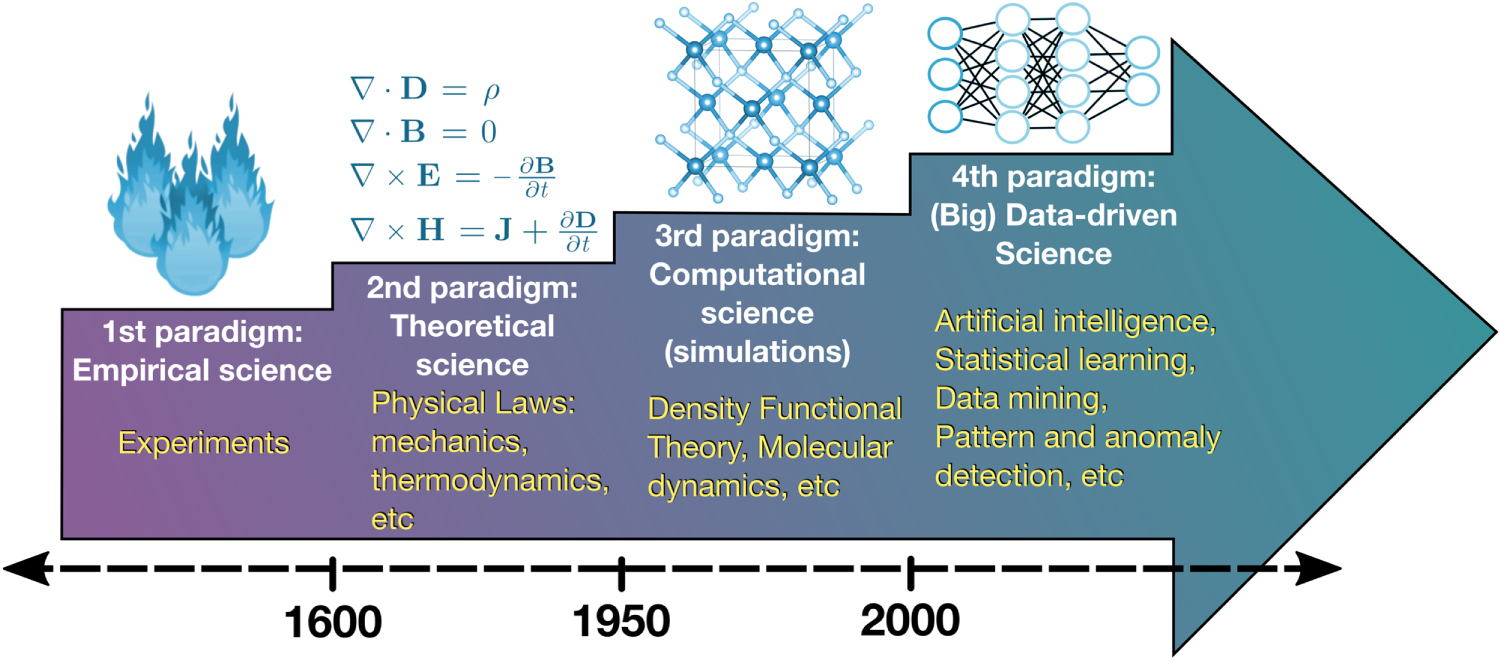
\includegraphics{theory/figures/4th-paradigm-hd.jpg}
  \caption{The four science paradigms: empirical, theoretical, computational, and data-driven. Figure taken from Ref.  \cite{Schleder2019}, which was originally adapted from Ref. \cite{Agrawal2016}.}
  \label{fig:4th-paradigm}
\end{figure}

This chapter aims to provide the neccessary understanding of the new research paradigm in the context of computational materials science and novel materials discovery. Starting from the beginning, we will be looking into information gained by \textit{ab initio} calculations, which means "from first principles". %In particular, it involves a summary of the neccessary theory behind the density functional theory, thus leaving most of the quantum-mechanical world untouched.
Since DFT is not a theory one simply understands, we will begin with an initial discussion of why it is difficult to calculate interactions between particles, followed by a review of key approximations and methods regarding the theory. However, even if density functional theory solves some problems, it also introduces new challenges, which will be thoroughly discussed.

Thereafter, we try to provide a logical sequence into the emergence of high-throughput (HT) methods and tools neccessary to handle the resulting information. Finally, we review a state-of-the-art approach of novel materials discovery enabled by the new paradigm of big data and data science.

\begin{comment}
\section{The single-electron Schrödringer equation}

We will start of investigating the Schrödinger equation with only one electron \cite{Griffiths2017}
\begin{align}
    i\hslash \frac{\partial \Psi}{\partial t} = -\frac{\hslash^2}{2m}\nabla^2 \Psi + V\Psi
    \label{eq:Schrödinger}
\end{align}
for a convenient external potential $V_{ext}(r)$ that is independent of time. We will try to look for solutions for (\autoref{eq:Schrödinger}) by separating the wave function into a space-dependent and time-dependent function
%Most wavefunctions are solutions to (\autoref{eq:Schrödinger}), but if the wavefunction describes a stationary state, the wavefunction has to be an eigenfunction to H for reasons that will become clear shortly.
\begin{align}
  \Psi(r,t) = \psi(r)\phi(t).
  \label{eq:separation}
\end{align}
By inserting ordinary derivatives and dividing each side with equation (\autoref{eq:separation}), our Schrödinger equation (\autoref{eq:Schrödinger}) now reads
\begin{align}
  i\hslash \frac{1}{\phi(t)}\frac{d\phi(t)}{dt} = - \frac{\hslash^2}{2m} \frac{1}{\psi(r)}\nabla^2 \psi + V(r)
\end{align}

Since the potential function $V(r)$ is independent of time, we observe the time and space dependencies of each side and state the fact that both sides has to be constant. Thus, two intriguing equations unveil themselves;
%captivating?
\begin{align}
  i\hslash \frac{1}{\phi(t)}\frac{d\phi(t)}{dt} = E\phi(t)
  \label{eq:time}
\end{align}
and
\begin{align}
  \frac{\hslash^2}{2m} \frac{1}{\psi(r)}\nabla^2 \psi + V(r) = E\psi(r)
  \label{eq:tise}
\end{align}
where the first equation (\autoref{eq:time}) has a general solution $\phi(t) = C \exp (-iEt/\hslash)$ and $C=1$ after normalization, and the second equation (\autoref{eq:tise}) is known as time-independent Schrödinger equation. These two equations are connected through the variable $\varepsilon$.

By utilizing variable separation to get equation (\autoref{eq:separation}), we find that the wavefunction is describing a stationary state with probability density
\begin{align*}
  \lvert \Psi (r,t)\rvert ^2 &= \Psi^*\Psi \\
  &= \Psi^* e^{iEt/\hslash} \Psi e^{-i Et/\hslash} \\
  &= \lvert \Psi (r)\rvert ^2
\end{align*}
that is independent of time. Conveniently, this is also true for every expectation value; they are all constant in time. We can also try to express this in classical terms regarding the Hamiltonian, which in this scenario is defined as
\begin{align}
    \hat{H}(r, p) = \frac{p^2}{2m} + V(r) = -\frac{\hslash^2}{2m}\nabla^2 + V(r)
\end{align}
simplifying equation \autoref{eq:tise} to
\begin{align}
  \hat{H} \psi = E\psi
  \label{eq:tise_nesten}
\end{align}
and we can find the expectation value of the total energy as
\begin{align*}
    \langle H \rangle &= \int \psi^* \hat{H} \psi dr \\
                &= E\int \lvert \Psi \rvert ^2 dr \\
                &= E
\end{align*}
using the fact that expectation values are constant in time for stationary states. Similarly, we can try to estimate the variance of the Hamiltonian,
\begin{align*}
  \sigma_H^2 &= \langle H^2 \rangle - \langle H \rangle ^2 \\
            &= E^2 - E^2 \\
            &= 0
\end{align*}
which appropiately describes that every measurement of the total energy is certain to return the value E.

\subsection{Eigenfunctions}
So far, we have not given an explanation of what a wavefunction is. As a matter of fact, we have actually found an eigenfunction
\begin{align*}
  \psi_\kappa(r,t) = \psi_\kappa e^{-i\varepsilon_\kappa t/\hslash}
\end{align*}
where $\kappa$ denotes the $k$-th eigenfunction and $\varepsilon_\kappa$ is its corresponding energy eigenvalue. The eigenfunctions have distinct energies and have the attribute that they are orthogonal and normalized with respect to
\begin{align*}
  \bra{\psi_\kappa (r,t)} \ket{\psi_{\kappa`} (r,t)} = \delta_{\kappa \kappa'}.
\end{align*}
The state with the lowest energy is called the ground state, and is where it is most likely to find an electron in a single-electron system with no external potential applied.

A general wavefunction can be generated by a summation of eigenfunctions (such as the eigenfunction in the latter case)
\begin{align}
\Psi(r,t) = \sum_\kappa c_\kappa \psi_{\kappa}(r,t),
\end{align}
where $c_\kappa$ is a constant. A general wavefunction does not neccessarily describe stationary states, and consequently does not have distinct energies but is rather represented statistically from the expectation value
\begin{align*}
  E = \sum_{\kappa} \lvert c_\kappa \rvert \varepsilon_\kappa.
\end{align*}
Solving Schrödinger equation for a general wavefunction is rather troublesome. Fortunately, we can use the eigenfunctions instead, transforming equation \autoref{eq:tise_nesten} into time-independent Schrödinger equation for eigenfunctions
\begin{align}
  \hat{H} \psi_{\kappa}(r) = \varepsilon_\kappa \psi_\kappa(r).
\end{align}

The shape of en eigenfunction has normally high spatial symmetri that depends on the symmetri of the potential $V_{ext}(r)$ and the boundary conditions \cite{Persson2020}. The study of how atoms in a crystalline interact with each other is of upmost importance when trying to explain macroscopic consequences.

\end{comment}
\section{Quantum mechanics}
%Before we
%Initially, the method of the calculations can be regarded as a black box where one provides the structure of a material as input, where the black box in return feeds us the outcome in terms of e.g. a different structure. The black box in question is based on a successful theory called density functional theory, which is an approach for predicting physical properties of solid-state systems. %In this and the next section we provide the neccessary knowledge to understand what is happening inside the black box, and the quality of the output.

To fully understand what challenges the density functional theory solves, we will need to introduce a few concepts in quantum mechanics. Quantum mechanics is the fundamental theory which describes nature at microscopic scale. We will only look at the neccessary theory needed to understand the DFT, leaving most of the theory in quantum mechanics untouched.

%Leading up to the density functional theory, we will initially introduce a few concepts required to understand it. Specifically, we will need to utilize the theory of quantum mechanics.

%The significance of this will be crystal clear when we later have to interpret information regarding several thousands solid-state systems, and not a single material. In particular, the quality of the output depends on being consistent.



%Before , we will need to investigate how we can calculate the forces acting inside a crystal. Since these forces are happening on a microscopic scale, we will need to utilize the theory of quantum mechanics.

%However, the fundamental theory remains the same and we will start our venture with the Schrödinger equation.


\subsection{The Schrödinger equation}

In principle, we can describe all physical phenomenas of a system with the wavefunction $\Psi(\boldsymbol{r},t)$ and the Hamiltonian $\hat{H}(\boldsymbol{r},t)$, where $\boldsymbol{r}$ is the spatial position and $t$ is the time. Unfortunately, analytical solutions for the the time-dependent Schrödinger equation,
\begin{align}
    i\hslash \frac{\partial}{\partial t} \Psi(\boldsymbol{r},t) = \hat{H}(\boldsymbol{r},t) \Psi(\boldsymbol{r},t),
    \label{eq:tdse}
\end{align}
are extremely rare. More conveniently, we can generate a general wavefunction by a summation of eigenfunctions,
\begin{align}
  \Psi(\boldsymbol{r},t) = \sum_\kappa c_\kappa \psi_\kappa(\boldsymbol{r},t),
\end{align}
where $c_\kappa$ is a constant and $\psi_\kappa$ is the $\kappa$-th eigenfunction. A general wavefunction does not have distinct energies but is rather represented statistically from the expectation value  %neccessarily describe stationary states, and consequently does not have distrinct energies but is rather represented statistically from the expectation value
\begin{align}
  \left \langle E \right \rangle = \sum_\kappa \lvert c_\kappa \rvert E_\kappa.
\end{align} Solving the Schrödinger equation for a general wavefunction is rather troublesome. However, for a time independent potential, we can use the eigenfunctions and transform \autoref{eq:tdse} into the time-independent Schrödinger equation for eigenfunctions by separation of variables, resulting in
\begin{align}
  \hat{H}\psi_\kappa(\boldsymbol{r}) = E_\kappa \psi_k(\boldsymbol{r}),
\end{align}
where $E_\kappa$ is the eigenvalue of the $\kappa$-th eigenstate $\psi_\kappa(\boldsymbol{r})$. The eigenfunctions have discrete energies, and the state with the lowest energy is called the ground state. They have the attribute that they are orthogonal and normalized with respect to
\begin{align}
  \left \langle \psi_\kappa \left(\boldsymbol{r}\right) \rvert \psi_{\kappa`} \left(\boldsymbol{r} \right) \right \rangle = \delta_{\kappa \kappa'}.
\end{align}
For more information, see Ref. \cite{Griffiths2017}.

\subsection{The many-particle Schrödinger equation}
As we extend the theory to include many-particle systems, we will gradually explain and add the different contributions that make up the many-body Hamiltonian. During this process, we will neglect any external potential applied to the system. \begin{comment}Furthermore, we will apply natural units, that is
\begin{itemize}
  \item Reduced planck constant $\hslash  = 1$.
  \item The magnitute of the charge of the electron $e = 1$.
  \item The electron rest mass $m_e = 1$.
  \item The coloumb force constant $(4\pi\varepsilon_0)^{-1}=1$.
\end{itemize}
\end{comment}

If we place a simple electron with mass $m_e$ in a vacuum, it will be in  possession of kinetic energy. Instead of just one electron, we can place $N_e$ electrons, and they will together have the total kinetic energy
\begin{align}
  T_e = - \sum_{j=1}^{N_e} \frac{\hslash^2\nabla_j}{2m_e}.
\end{align}
All the electrons are negatively charged, causing repulsive Coulomb interactions between each electron, totalling to
\begin{align}
  U_{ee} = \frac{1}{4\pi\varepsilon_0}\sum_{j=1}^{N_e}\sum_{j'<j} \frac{q^2}{\lvert r_j - r_{j'}\rvert},
  \label{eq:electron-electron}
\end{align}
where $\varepsilon$ is the vacuum permittivity. The summation avoids counting each interaction more than once. Simultaneously, we can place $N_n$ nuclei with mass $m_n$ in the same system, accumulating the kinetic energy
\begin{align}
  T_n = - \sum_{a=1}^{N_n} \frac{\hslash^2\nabla_a}{2m_n}.
\end{align}
As in the example with electrons, the nuclei are also experiencing repulsive interactions between every single nucleus, adding up the total interactions as
\begin{align}
  U_{nn} = \frac{1}{4\pi\varepsilon_0}\sum_{a=1}^{N_n}\sum_{a'<a} \frac{q^2 Z_aZ_{a'}}{\lvert R_a - R_{a'}\rvert }.
\end{align}
where $Z_a$ is the atom number of nuclei number $a$. The system now contains $N_e$ electrons and $N_n$ nuclei, thus we need to include the attractive interactions between the them,
\begin{align}
  U_{en} = - \frac{1}{4\pi\varepsilon_0}\sum_{j=1}^{N_e} \sum_{a=1}^{N_n} \frac{q^2Z_a}{\lvert r_j-R_a\rvert}.
\end{align} Together, these equations comprise the time-independent many-particle Hamiltonian
\begin{align}
  \begin{aligned}
    \hat{H} = &- \sum_{j=1}^{N_e} \frac{\hslash^2\nabla_j}{2m_e}
    - \sum_{a=1}^{N_n} \frac{\hslash^2\nabla_a}{2m_n}
    + \frac{1}{4\pi\varepsilon_0} \sum_{j=1}^{N_e}\sum_{j'<j} \frac{q^2}{\lvert r_j - r_{j'}\rvert} \\
    &+\frac{1}{4\pi\varepsilon_0}\sum_{a=1}^{N_n}\sum_{a'<a} \frac{q^2 Z_aZ_{a'}}{\lvert R_a - R_{a'}\rvert } - \frac{1}{4\pi\varepsilon_0}\sum_{j=1}^{N_e} \sum_{a=1}^{N_n} \frac{q^2Z_a}{\lvert r_j-R_a\rvert}.
  \end{aligned}
\end{align} A few problems arise when trying to solve the many-particle Schrödinger equation. Firstly, the amount of atoms in a crystal is very, very massive. As an example, we can numerically try to calculate \autoref{eq:electron-electron} for a $1$ mm$^3$ silicon-crystal that contains $7\cdot 10^{20}$ electrons. For this particular problem, we will pretend to use the current fastest supercomputer Fugaku \cite{Top500} that can calculate $514$ TFlops, and we will assume that we need $2000$ Flops to calculate each term inside the sum \cite{Persson2020}, and we need to calculate it $N_e \cdot N_e/2$ times for the (tiny) crystal.
The entire electron-electron interaction calculation would take $2.46 \cdot 10^{19}$ years to finish for a tiny crystal. Thus, the large amount of particles translates into a challenging numerical problem.

%In one cubic-centimeter of a crystal, there are around $10^{23}$ electrons. This number is roughly the same as the number of stars in the universe, grain of sand on all beaches in the world, or currently $1.41\cdot 10^{19}$ times the amount of Home and Away episodes made since 1988.

Secondly, the many-particle Hamiltonian contains operators that has to be applied to single-particle wavefunctions, and we have no prior knowledge of how $\Psi$ depends on the single-particle wavefunctions $\psi_\kappa$.


\subsection{The Born-Oppenheimer approximation}
The many-particle eigenfunction describes the wavefunction of all the electrons and nuclei and we denote it as $\Psi_{\kappa}^{en}$ for electrons (e) and nuclei (n), respectively. The Born-oppenheimer approximation states that nuclei, of substantially larger mass than electrons, can be treated as fixed point charges. According to this assumption, we can separate the eigenfunction into an electronic part and a nuclear part,
\begin{align}
  \Psi_\kappa^{en}(\boldsymbol{r}, \boldsymbol{R}) \approx \Psi_{\kappa}(\boldsymbol{r}, \boldsymbol{R})\Theta_{\kappa}(\boldsymbol{R}),
\end{align}
where the electronic part is dependent on the nuclei. This is in accordance with the assumption above, since electrons can respond instantaneously to a new position of the much slower nucleus, but this is not true for the opposite scenario. By utilizing this approximation, it can be shown that the equation can be separated into an electronic and a nuclear eigenvalue equation,

\begin{align}
      \left( T_e + U_{ee} + U_{en} \right) \Psi_\kappa (\boldsymbol{r},\boldsymbol{R}) &= E_{\kappa}(\boldsymbol{R})\Psi_\kappa(\boldsymbol{r},\boldsymbol{R})\\
      \left(T_n + U_{nn} + E_\kappa (\boldsymbol{R}) \right) \Theta_\kappa(\boldsymbol{R}) &= E_{\kappa}^{en}(\boldsymbol{R})\Theta_\kappa(\boldsymbol{r},\boldsymbol{R}),
\end{align}
where the two equations are coupled by the electronic energy eigenvalue $E_{\kappa}(\boldsymbol{R})$. Since we can consider the nuclei as point charges, it is common to set the kinetic energy of the nuclei, $T_n$, to zero. Thus, the left side of the nuclear eigenvalue equation is shortened down to the terms $\left(U_{nn} + E_\kappa (\boldsymbol{R}) \right)$, which is denoted as the potential energy surface (PES), $E_p(\boldsymbol{R})$.
%From here, one can obtain the electronic and nuclear eigenfunction, with the derivation shown in Appendix \ref{appendix:Born-Oppenheimer}.


\subsection{The Hartree and Hartree-Fock approximations}
\begin{comment}
As we venture along from a one-electron system to a two-electron systen, we encounter a new wavefunction and Hamiltonian that needs to describe two particles, making the two-electron Schrödinger equation read

\begin{align}
  \Big( -\frac{\hslash^2 \nabla_1^2}{2m_e} - \frac{\hslash^2\nabla_2^2}{2m_e}+ \frac{q^2}{\lvert r_1-r_2  \rvert} + V_{ext}(r) \Big) \Psi_\kappa (r_1, r_2) = E_{\kappa} \Psi_\kappa (r_1, r_2),
\end{align}
where the two first terms are the kinetic energies of the electrons, while the third term is a potential that describes the repulsive Coloumb interaction between the two electrons. The last term is the external potential, well known from the earlier scenario with only one electron.
\end{comment}
The next question in line is to find a wavefunction $\Psi(\boldsymbol{r},\boldsymbol{R})$ that describes all of the electrons in the system. The Hartree \cite{Persson2020, DavidSholl2009} approximation to this is to assume that electrons can be described independently, suggesting the \textit{ansatz} for a two-electron wavefunction
\begin{align}
  \Psi_\kappa(\boldsymbol{r}_1,\boldsymbol{r}_2) = A \cdot \psi_1(\boldsymbol{r}_1) \psi_2(\boldsymbol{r}_2),
\end{align}
where $A$ is a normalization constant. This approximation simplifies the many-particle Shrödinger equation a lot, but comes with the downside that the particles are distinguishable and do not obey the Pauli exclusion principle for fermions.

The Hartree-Fock approach, however, overcame this challenge and presented an anti-symmetric wavefunction that made the electrons indistinguishable \cite{Griffiths2017}:
\begin{align}
  \Psi_\kappa(\boldsymbol{r}_1,\boldsymbol{r}_2) = \frac{1}{\sqrt{2}}\Big( \psi_1(\boldsymbol{r}_1) \psi_2(\boldsymbol{r}_2)  - {\psi_1(\boldsymbol{r}_2)\psi_2(\boldsymbol{r}_1)}\Big).
\end{align}
%For systems containing more than one particles, the factor $1/\sqrt{2}$ becomes the Slater determinant and is used to normalize the wave function.

\subsection{The variational principle}
So far, we have tried to make the time-independent Schrödinger equation easier with the use of an \textit{ansatz}, but we do not neccessarily have an adequate guess for the eigenfunctions and the ansatz can only give a rough estimate in most scenarios. Another approach, namely the \textit{variational principle}, states that the energy of any trial wavefunction is always an upper bound to the exact ground state energy by definition $E_0$,
\begin{align}
  E_0 = \bra{\psi_0 } H \ket{\psi_0} \leq \bra{\psi}H\ket{\psi} = E
  \label{eq:variational}
\end{align} This enables a minimization of energy in terms of wavefunction parameters. A more thorough walk-through of the variational principle is included in Appendix \ref{appendix:variational-principle}.

\section{The density functional theory}

Hitherto we have tried to solve the Schrödinger equation to get a ground state wave function, and from there we can obtain ground state properties. One fundamental problem that exists when trying to solve the many-electron Schrödinger equation is that the wavefunction is a complicated function that depends on $3N_e$ variables\footnote{not including spin}.

Hohenberg and Kohn \cite{Hohenberg1964} showed in 1964 that the ground-state density $n_0(r) = \lvert \Psi_0 (r)\rvert$ determines a general external potential, which includes $U_{en}$, up to an additive constant, and thus also the Hamiltonian \cite{Toulouse2019}. From another point of view, the theory states that all physical ground-state properties of the many-electron system are unique functionals of the density \cite{Persson2020}. A consequence of this is that the number of variables is reduced from $3N_e$ to $3$, significantly reducing the computational efforts.

However, the scheme is not without limitations, as the density functional theory (DFT) can only be used to find all the ground-state physical properties if the exact functional of the electron density is known. And $57$ years after Hohenberg and Kohn published their paper, the exact functional still remains unknown.

We will start this chapter with a brief mention of the Hohenberg-Kohn theorems and its implications, before we delve further into the Kohn-Sham equation.

\subsection{The Hohenberg-Kohn theorems}

\begin{theorem}
  For any system of interacting particles in an external potential $V_{ext}$, the density is uniquely determined.
\end{theorem}

The theorem can be proved by utilising the variational principle for two different external potentials with the same ground state density.
The proof is included in Appendix \ref{appendix:theorem1}.

\begin{theorem}
  There exists a variational principle for the energy density functional such that, if $n$ is not the electron density of the ground state, then $E\left[ n_0 \right] < E\left[ n \right]$.
\end{theorem}

From theorem 1, we know that the external potential is uniquely determined by the density, which in turn uniquely determines the ground state wavefunction. Therefore, all other observables of the system are uniquely determined and we can express the energy as function of the density,
\begin{align}
  E[n] = \overbrace{T[n] + U_{ee}[n]}^{F[n]} + U_{en}[n],
  \label{eq:densityfunctional}
\end{align}
where $F[n]$ is an universel functional known as the Hohenberg-Kohn functional. The proof for theorem 2 is found in Appendix \ref{appendix:theorem2}.

\subsection{The Kohn-Sham equation}
So far, we have tried to make the challenging Schrödinger equation less challenging by simplifying it. The last attempt of simplifying it involved the Hohenberg-Kohn's theorems where the theory states that the total ground-state energy can, in principle, be determined exactly once we have found the ground-state density.

In 1965, Kohn and Sham \cite{Kohn1965} reformulated the Hohenberg-Kohn theorems by generating the exact ground-state density $n_0(r)$ using a Hartree-like total wavefunction
\begin{align}
    \Psi(\boldsymbol{r}_1,\boldsymbol{r}_2,..,\boldsymbol{r}_{N_e}) = \psi_1^{KS}(\boldsymbol{r}_2)\psi_2^{KS}(\boldsymbol{r}_2)...\psi_{N_e}^{KS}(\boldsymbol{r}_{N_e}),
\end{align}
where $\psi_j^{KS}(r_j)$ are some auxiliary independent single-particle wavefunctions. However, the Kohn-Sham wavefunctions cannot be the correct single-particle wavefunctions since our ansatz implies an exact density
\begin{align}
  n(\boldsymbol{r}) = \sum_{j=1}^{N_e}\lvert \psi_j^{KS}(\boldsymbol{r})\rvert^2.
\end{align}
Recalling that equation \autoref{eq:densityfunctional} describes the total energy as a functional of the density,
\begin{align}
  E[n] = T[n] + U_{ee}[n] + U_{en}[n],
\end{align}
we try to modify it to include the kinetic energy $T_s[n]$ and the interaction energy $U_s[n]$ of the auxiliary wavefunction, with the denotation $s$ for single-particle wavefunctions.
\begin{align*}
  E[n] &= T[n] + U_{ee}[n] + U_{en}[n] + \left( T_s[n] - T_s[n] \right) + \left( U_s[n] - U_s[n] \right) \\
  &= T_s[n] + U_{s}[n] + U_{en}[n] + \underbrace{\left(T[n] - T_s[n] \right) + \left( U_{ee}[n] - U_s[n] \right)}_{E_{xc}[n]}
\end{align*}
Here we have our first encounter with the \textit{exchange-correlation energy}
\begin{align}
  E_{xc}[n] = \Delta T + \Delta U = \left(T[n] - T_s[n] \right) + \left( U_{ee}[n] - U_s[n] \right),
\end{align}
which contains the complex many-electron interaction. For non-interacting systems, $E_{xc}[n]$ is conveniently zero, but in interacting systems it most likely is a complex expression. However, one can consider it as our mission to find good approximations to this term, as the better approximations, the closer we get to the exact expression.

The exact total energy functional can now be expressed as
\begin{align}
  \begin{aligned}
  E[n]
  &= \overbrace{\sum_j \int \psi_j^{KS*} \frac{-\hslash^2\nabla^2}{2m} \psi_j^{KS}d\boldsymbol{r}}^{T_s[n]} + \overbrace{\frac{1}{2}\frac{1}{4\pi\varepsilon_0}\int \int q^2\frac{n(\boldsymbol{r})n(\boldsymbol{r}')}{\lvert \boldsymbol{r}-\boldsymbol{r}'\rvert} d\boldsymbol{r}d\boldsymbol{r}'}^{U_s[n]}
  \\ &+ \underbrace{\int V_{en}(\boldsymbol{r})n(\boldsymbol{r})d\boldsymbol{r}}_{U_{en}[n]} + \underbrace{\left(T[n] - T_s[n] \right) + \left( U_{ee}[n] - U_s[n] \right)}_{E_{xc[n]}},
  \end{aligned}
\end{align}
given that the exchange-correlation functional is described correctly. By utilizing the variational principle, we can now formulate a set of Kohn-Sham single-electron equations,
\begin{align}
  \left\{ -\frac{\hslash^2}{2m_e}\nabla^2_s + V_H(\boldsymbol{r}) + V_{en}(\boldsymbol{r}) + V_{xc}(\boldsymbol{r}) \right\} \psi_s^{KS}(\boldsymbol{r}) = \epsilon_s^{KS} \psi_s^{KS}(\boldsymbol{r}),
  \label{eq:singleKS}
\end{align}
where $V_{xc}(\boldsymbol{r})=\partial E_{xc}[n]/\partial n(\boldsymbol{r})$ and $V_{H}(\boldsymbol{r})=\frac{1}{4\pi\varepsilon_0}\int q^2 \frac{n(\boldsymbol{r'})}{\lvert \boldsymbol{r} - \boldsymbol{r}'\rvert} d\boldsymbol{r}'$ is the Hartree potential describing the electron-electron interaction.
It is worth to notice that $V_H(\boldsymbol{r})$ allows an electron to interact with itself, resulting in a self-interaction contribution, however this can be taken care of in $V_{xc}$.

Finally, we can define the total energy of the system according to Kohn-Sham theory as
\begin{align}
  E[n] = \sum_{j}\epsilon_j^{KS}-\frac{1}{2}\frac{1}{4\pi\varepsilon_0}\int \int q^2 \frac{n(\boldsymbol{r})n(\boldsymbol{r}')}{\lvert \boldsymbol{r} - \boldsymbol{r}' \rvert} d\boldsymbol{r}d\boldsymbol{r}' + E_{xc}[n] - \int V_{xc}(\boldsymbol{r})n(\boldsymbol{r})d\boldsymbol{r}.
\end{align}
If $V_{xc}$ is exact, and $E[n]$ gives the true total energy, we still do not know if the energy eigenvalues $\epsilon_s^{KS}$ are the true single-electron eigenvalues. However, there exists one exception, which is that the highest occupied eigenvalue of a finite system has to be exact if the density is exact.

The only task that is left for us now is to find the exact expression for $E_{xc}[n]$ as a functional of the density $n(r)$. With that expression, we would be able to calculate the total energies of any material. %, and most likely solve a few of the biggest puzzles in the history of humankind.
Unfortunately, the exchange-correlation potential is unknown for most systems.

It is possible to solve the Kohn-Sham equations by applying a self-consistent field method. This is a computational scheme, and for further details one can consult the Appendix \ref{appendix:self-consistent}.

%In this approximation we have used Hartree energy where the self-interaction correction is neglected, raising less accurate results. It is possible to use other approximations for $T_s[n]$ and $U_s[n]$ than Hartree wavefunctions, and good approximations will result in a low $E_{xc}[n]$ because $T_s[n]$ and $U_s[n]$ will get closer and closer to the true values.


%The next step in finding the KS-equation is to utilize the variational principle in the purpose of finding the ground-state energy. First one minimises the total energy with respect to each of the wavefunctions with the constraint that the wavefunctions should be orthonormalized;
%\begin{align*}
%  \frac{\partial }{\partial \psi_j^{*} (\boldsymbol{r})}E[n] &= \sum_{i,j}\lambda_{ij}\int \psi_i^{s*}(\boldsymbol{r}_i)\psi_j^{s}(\boldsymbol{r}_j)d\boldsymbol{r}d\boldsymbol{r}_j\\
%  \frac{\partial }{\partial \psi_j^{*} (\boldsymbol{r})}E[n] &= \lambda_j\psi_j^s (\boldsymbol{r}_j)
%\end{align*}

\subsection{The exchange-correlation energy}


There is one scenario for which we can derive the exact expression of the exchange-correlation functional, namely the \textit{homogeneous electron gas} (HEG). However, this has a natural cause, since by definition $n(\boldsymbol{r})$ is constant for this situation. Given that it is the variations of electron density that are the foundation of material properties, the usefulness of HEG is limited. The \textit{local density approximation} (LDA) is an approximation based on this approach, where the local density is the only variable used to define the exchange-correlation functional. Specifically, we can set the exchange-correlation potential at each position to be the known exchange-correlation potential from homogeneous electron gas at the electron density observed at that position \cite{Kohn1965}:
\begin{align}
  V_{xc}(\boldsymbol{r}) = V_{xc}^{\text{electron gas }}\left[n(\boldsymbol{r})\right].
\end{align}
This is the simplest and most known approximation to the exchange-correlation functional, and accordingly it has a few drawbacks. One of them is the incomplete cancellation of the self-interaction term, which leads to a repulsion that may cause artifical repulsion between electrons, and hence increased electron delocalization \cite{Allen2014}. In addition, LDA has proven challenging  to use when studying atoms and molecules because of their rapidly varying electron densities, however, the LDA is seen as succesful for bulk materials because of the slowly varying electron density \cite{DavidSholl2009}. Considering the relatively low computational cost and relatively high accuracy, the LDA overall makes a good model for estimation of the exchange-correlation functional for bulk-materials.

In the light of the merits of the LDA, an extensive search for new approximations was launched. The \textit{generalized gradient approximation} (GGA) is an extension of the LDA, which includes the gradient of the density
\begin{align}
  V_{xc}^{GGA}(\boldsymbol{r}) = V_{xc}\left[ n(\boldsymbol{r}), \nabla n (\boldsymbol{r})\right].
\end{align}
The GGA is a good approximation for the cases where the electron density varies slowly, but faces difficulties in many materials with rapidly varying gradients in the density, causing the GGA to fail. Thus, the annotation \textit{generalized} in GGA is set to include the different approaches to deal with this challenge. Two of the most commonly implemented GGA functionals are the non-empirical approaches Perdew-Wang 91 (PW91) \cite{Perdew1992} and Perdew-Burke-Ernzerhof (PBE) \cite{Perdew1996}.

Both LDA and GGA are commonly known to severely underestimate the band gaps of semiconductor materials, in addition to incorrectly predicting charge localizations originating from narrow bands or associated with local lattice distortions around defects \cite{Freysoldt2014}. The latter limitation is thought to be due to self-interaction in the Hartree potential in \autoref{eq:singleKS}.
\begin{comment}
To improve the accuracy of excited state properties estimations, other methods have been developed. Tran and Blaha (TB) \cite{Tran2009} adapted the exchange potential suggested by Becke-Roussel (BR) \cite{Becke2006} that leads to band gaps close to experimental values while still using a cheap semilocal method \cite{Koller2011}. The modified TB-mBJ version introduces a parameter relative to the BJ version,
\begin{align}
    V_{xc}^{TB-mBJ}(\boldsymbol{r}) =  c\cdot V_{xc}^{BR}(\boldsymbol{r}) + (3c-2) \frac{1}{\pi} \sqrt{\frac{5}{6}} \sqrt{\frac{t(\boldsymbol{r})}{\rho(\boldsymbol{r})}},
\end{align}
where $\rho$ is the electron density, $t$ is the kinetic-energy density, $V_{xc}^{BR}$ is the Becke-Roussel exchange potential and $c$ is the parameter that changes weights of the BJ potential and is fit to experimental data.
\end{comment}
Hybrid functionals intermix exact Hartree-Fock exchange with exchange and correlation from functionals based on the LDA or GGA. Hartree-Fock theory completely ignores correlation effects, but accounts for self-interaction and treats exchange as exact. Since LDA/GGA and Hartree-Fock supplement each other, they can be used as a combination for hybrid-functionals resulting in some cancellation of the self-interaction error. Becke \cite{Becke1993} introduced a $50\%$ Hartree-Fock exact exchange and
$50\%$ LDA energy functional, while Perdew \textit{et al.} \cite{Perdew1996a} altered it to $25\%-75\%$ and favoring PBE-GGA instead of LDA.

The inclusion of Hartree Fock exchange improves the description of localized states, but requires significantly more computational power for large systems. Another method called the \textit{GW} approximation includes screening of the exchange interaction \cite{Aryasetiawan1998}, but has a computational price that does not neccessarily defend its use. Thus, the real challenge is to reduce the computational effort while still producing satisfactory results. Heyd \textit{et al.} \cite{Heyd2003} suggested to separate the non-local Hartree-Fock exchange into a short- and long-range portion, incorporating the exact exchange in the short-range contribution. The separation is controlled by an adjustable parameter $\omega$, which was empirically optimised for molecules to $\omega = 0.15$ and solids to $\omega = 0.11$ and are known as the HSE03 and HSE06 (Heyd-Scuseria-Ernzerhof), respectively \cite{Krukau2006}. The functionals are expressed as
\begin{align}
  E_{xc}^{HSE} = aE_{x}^{\text{HF,SR}}(\omega) + (1-a)E_x^{\text{PBE,SR}}(\omega) + E_x^{\text{PBE,LR}}(\omega) + E_c^{\text{PBE}}
\end{align}
where $a=1/4$ is the Hartree-Fock mixing constant and the abbreviations SR and LR stands for short range and long range, respectively.

Hence, hybrid-functionals are \textit{semi-empirical} functionals that rely on experimental data for accurate results. They give accurate results for several properties, such as energetics, bandgaps and lattice parameters, and can fine-tune parameters fitted to experimental data for even higher accuracy.

Furthermore, the computational effort required for the hybrid-functionals are significantly larger than for non-empirical functionals such as LDA or GGA. Krukau \textit{et al.} \cite{Krukau2006} reported a substantial increase in computational cost when reducing the parameter $\omega$ from $0.20$ to $0.2$ for 25 solids, and going lower than $0.11$ demanded too much  to actually defend its use.
\begin{comment}
Unfortunately, an area where both GGA and hybrid functionals are reportedly inadequate is in calculating the dispersion interactions \cite{Klimes2009}. Many implementations have been developed to deal with this vulnerability, with one of them being the non-local van der Waals density functional (vdW-DF) \cite{Dion2004}
\begin{align}
  E_{xc} = E_{x}^{GGA} + E_{c}^{\text{LDA}} + E_{c}^{nl},
\end{align}
where $E_{x}^{GGA}$ is GGA exchange energy \cite{Klimes2009}.
\end{comment}
\subsection{Limitations of the DFT}

If we had known the exact exchange-correlation functional, the density functional theory would yield the exact total energy. Alas, that is not the case and we are bound to use approximations in forms of functionals. What is common for all approximations is that they are specifically designed to solve one given optimization in DFT, therefore it is not neccessarily one functional that is considered superior in all fields of interest. One could consider that the hybrid functionals due to a high accuracy overall should be dominant, but that is only if one has the computational capacity required. The accuracy of calculations depends on which functional is used, and normally a higher accuracy means the use of a more complex and computationally demanding functional.

Additionally, one can almost never be certain if a DFT-calculation has found a local or global minima. There is an unknown associated uncertainty of every calculation, which has to be taken into consideration. Nonetheless, density functional theory is considered a very successful approach and Walter Kohn was awarded the Nobel Price in chemistry in 1998 for his development of the density-functional theory \cite{Freitas1999}. It has matured into the undisputed choice of method for electronic structure calculations \cite{Schleder2019}. It is especially regarded as successful in contexts where DFT can make important contributions to scientific questions where it would be essentially impossible to determine through experiments \cite{DavidSholl2009}. %One can only hope that the future will be as bright as the past, and that this successful theory provides incentives for further growth in the next generation.

\section{High-throughput information storage}


Fuelled by the widespread application of DFT in material science, we observe an increase of computational capacity due to advances in simulation methods, computational science and technologies \cite{Schleder2019}. The time required for calculations has been reduced substantially, and enables more time to be spent on simulation setup and analysis. Ultimately, this has led to a new type of workflow called high-throughput (HT) \cite{Yang2017}, where one can automate input creation and perform several (up to millions) simulations in parallel instead of performing many manually-prepared simulations. The HT engines are required to be fast and accurate, otherwise the purpose of its existence is lost. We will in this thesis mainly focus on high throughput in the context of first principles DFT calculations.

Normally, the implementation of HT-DFT methods is done in three steps. In the first step we perform thermodynamic or electronic structure calculations for a large number of materials. For the second step, we store the information gathered in a systematic database, normally known as a material repository. For the third and final step, we characterize and select novel materials or analyse and extract new physical insight \cite{Schleder2019}. In general, the two first steps are performed on high-performance computers (HPC), and are defining for the third step due to the vast amount of interesting properties of materials. Importantly, one needs to consider the ultimate goal in step three initially before deciding upon materials and properties to calculate.

One of the largest government funded projects is the $2011$ launched Material Genome Initiative (MGI) \cite{Warren2018} which seeks to accelerate the discovery, design, development and deployment of novel materials through the creation of a materials innovation infrastructure.
As a result, we have seen an intensive implementation of material repositories that fascilitate sharing and distribution of step $1$ and $2$, with the ultimate goal of storing calculated properties of all feasible structures of materials \cite{Schuett2020}.
Examples include AFLOW \cite{Curtarolo2012, Curtarolo2012a, Calderon2015}, Materials Project \cite{Jain2013, Jain2018} , OQMD \cite{Saal2013, Kirklin2015} and JARVIS-DFT \cite{Choudhary2020}.
On the other hand, we find a less diverse selection of experimental databases, with perhaps the most known being the Inorganic Crystal Structure Database (ICSD) \cite{Allen1987}.

In this section, we describe a few of the most widely known high-throughput databases, codes and tools, with an emphasis of what the particular speciality of each database is.

\subsection{Materials project}

Materials project \cite{Jain2013, Jain2018} is an open source project that is based on the Vienna Ab Initio Software Package (VASP) \cite{Kresse1996}, and offers a variety of properties of over one hundred thousand inorganic crystalline materials. It is known as the initiator of materials genomics and has as its mission to accelerate the discovery of new technological materials, with an emphasis on batteries and electrodes, through advanced scientific computing and innovative design.

 %Some features, eg. density of state (dos), bandstructure, Pourbaix diagram etc., are characterized by using the module pymatgen.

Every compound has an initial relaxation of cell and lattice parameters performed using a $1000$ / (number of atoms in cell) k-point mesh to ensure that all properties calculated are representative of the idealized unit cell for each respective crystal structure \cite{Ferrenti2020}. The functional GGA is used to calculate band structures, while for transition metals, a $+U$ corrections is applied to correct for correlation effects in d- and f-orbital systems that are not addressed by GGA calculations \cite{Wang2006}.

To adress that many compounds are not thermodynamically stable, which means that they do not appear on any phase stability diagrams \cite{Sun2016}, an additional metric has been added. This metric is based on a convex hull analysis, where compounds on the convex hull are stable, while compounds above the hull in terms of energy are metastable \cite{Jain2018}. This is denoted as energy above hull (E Above Hull), where a value of zero is defined as the most stable phase at a given composition, while larger positive values indicate increased instability.

%The thermodynamic stability for each phase with respect to decomposition, is also calculated.
Each material contains multiple computations for different purposes, resulting in different 'tasks'. The reason behind this is that each computation has a purpose, such as to calculate the band structure or energy. Therefore, it is possible to receive several tasks for one material.

\subsection{AFLOW}

The AFLOW\cite{Curtarolo2012, Curtarolo2012a, Calderon2015} repository is an automatic software framework for the calculations of a wide range of inorganic material properties. They utilise the GGA-PBE functional within VASP with projector-augmented wavefunction (PAW) potentials to relax twice and optimize the ICSD-sourced structure. They are using a $3000$ to $6000$ / (number of atoms in cell) $k$-point mesh, indicating a more computationally expensive calculation compared to the Materials Project \cite{Ferrenti2020}. Next, the band structure is calculated with an even higher $k$-point density, in addition to the $+U$ correction term for most occupied d- and f-orbital systems \cite{Setyawan2010}. Furthermore, they apply a standard fit gathered from a study of DFT-computed versus experimentally measured band gap widths to the initial calculated value, obtaining a fitted band gap \cite{Setyawan2011}.

\subsection{Open Quantum Materials Database}

The Open Quantum Materials Database (OQDM) \cite{Saal2013, Kirklin2015} is a free and available database of DFT-calculations. It contains thermodynamic and structural properties of more than $600.000$ materials, including all unique compounds in the Inorganic Crystal Structure Database (ICSD) that consists of less than $34$ atoms \cite{Ferrenti2020}.

The DFT calculations are performed with the VASP software whereas the electron exchange and correlation are described with the GGA-PBE, while using the PAW potentials. They relax a structure using $4000-8000$ / (number of atoms in cell) $k$-point mesh, indicating an even more computationally expensive calculation than AFLOW \cite{Ferrenti2020}. Several element-specific settings are included such as using the $+U$ extension for various transition metals, lanthanides and actinides. In addition, any calculation containing 3d or actinide elements are spin-polarized with a ferromagnetic alignment of spins to capture possible magnetism. However, the authors note that this approach does not capture complex magnetic properties such as antiferromagnetism, which has been found to result in substantial errors for the formation energy \cite{Stevanovic2012}.

\subsection{JARVIS}

Joint Automated Repository for Various Integrated Simulations (JARVIS) - DFT \cite{Choudhary2020} is an open database based on the VASP \cite{Kresse1996} software to perform a variety of material property calculations. It consists of roughly $40.000$ 3D and $1.000$ 2D materials using the vdW-DF-OptB88 van der Waals (vdW) functional, which was originally designed to improve the approximation of properties of two-dimensional van der Waals materials, but was also shown to be effective for bulk materials \cite{Thonhauser2007, Klimes2011}. The functional has yielded accurate predictions for lattice-parameters and energetics for both vdW and non-vdW bonded materials  \cite{Choudhary2018}.

Structures included in the data set are originally taken from the Materials Project, and then re-optimized using the OPT-functional. Finally, the combination of the OPT and modified Becke-Johnson (mBJ) functionals are used to obtain a representative band gap of each structure \cite{Choudhary2018a}. %, since both have shown unprecedented accuracy in the calculation of band gap compared to any other DFT-based calculation methods \cite{Choudhary2018a}.
The JARVIS-DFT database is part of a bigger platform that includes JARVIS-FF, which is the evaluation of classical forcefield with respect to DFT-data, and JARVIS-ML, which is a repository of machine learning model parameters and descriptors.
%which consists of 25 machine learning descriptors to predict properties of materials.
In addition, JARVIS-DFT also includes a data set of 1D-nanowire and 0D-molecular materials, which is not yet publically distributed.

\section{Materials informatics}

Despite a computationally demanding step $1$ and a sophisticated database architecture defined in step $2$, the third step remains more important in discovery of novel materials. In the third step, we apply constraints to the database in order to filter or select the best candidates according to the desired attributes \cite{Schleder2019}, and is referred to as data \textit{mining} and data \textit{screening}. To achieve the most insight, we normally apply the constraints in a sequential manner to identify any potential underlying trend. The materials that satisfy the first constraint move on to the next round, while the rest are eliminated from further consideration. The constraints can be applied either by the understanding of properties, human intuition or through a close interaction with a machine learning (ML) algorithm, where the latter will be extensively studied in the next chapter.

\begin{figure}[ht!]
  \centering
  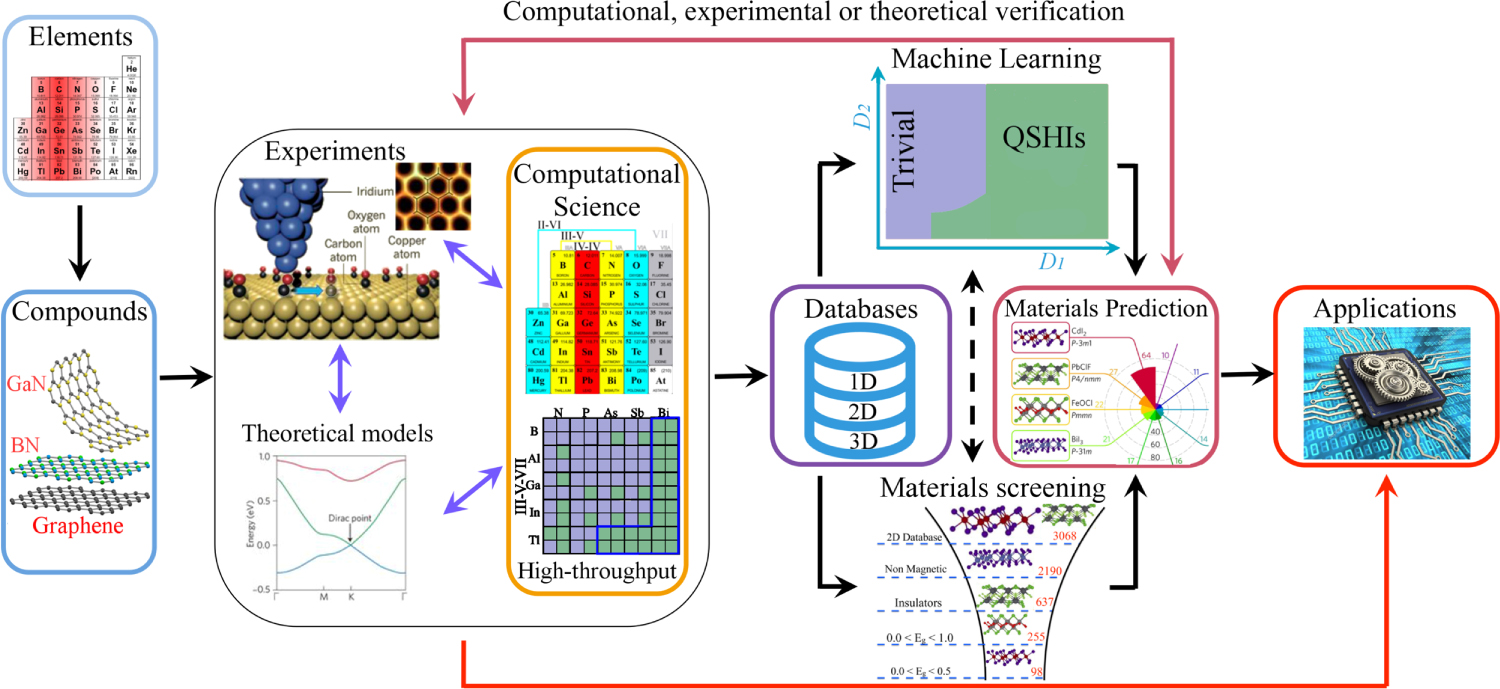
\includegraphics{theory/figures/ht-workflow.jpg}
  \caption{Schematic representation of the workflow of novel materials discovery.  Figure taken from Ref. \cite{Schleder2019}, which was originally adapted from Refs. \cite{Mounet2018, Acosta2018, Polini2013}.}
  \label{fig:ht-workflow}
\end{figure}

\noindent Together, the three steps resemble \autoref{fig:ht-workflow}. From building compounds based on elements, calculating theoretical, computational and experimental properties, storing the information in databases and applying material screening and machine learning, to finally receiving a material prediction. If the material prediction is verified iteratively by many independent sources, the time to market for new technologies based on a new material takes approximately $20$ years \cite{Eagar1995, Schleder2019}.

Importantly, the data driven paradigm enables a new approach for novel material discovery. The traditional approach, namely the \textit{direct approach}, relies on the calculation of properties given the structure and composition of a material, such that the search for eligible candidates exhibiting the target property is performed tediously case by case. In other words, what is the property of a given material. However, the \textit{inverse approach} is of integral importance in this work: given a desired property, what material can present it \cite{Schleder2019}?

The application of machine learning and data-driven techniques to material science has developed into a new field named \textit{materials informatics} \cite{Rajan2005}. Alex Szalay, director of the US National Virtual Observatory project, described informatics for astronomy in $2003$ as the following:
\begin{quote}
   ``Science was originally empirical, like Leonardo making wonderful drawings of nature. Next came the theorists who tried to write down equations that explained observed behaviors, like Kepler or Einstein. Then, when we got to complex enough systems like the clustering of a million galaxies, there came the computer simulations – the computational branch of science. Now, we are getting into the data exploration part of science, which is kind of a little bit of them all'' Alex Szalay \cite{Szalay2003}
\end{quote}
\noindent The formulation is true also for materials informatics, where the scope is to discover relations between known standard features and material properties through a combination of \emph{a bit of everything}.

\subsection{Materials informatics software packages}

In practice, several software packages exists for the purpose of generating, describing, visualizing, calculating or predicting properties of materials.

The Atomic Simulation Environment (ASE) is an environment in the Python programming language that includes several tools and modules for setting up, modifying and evaluate atomistic simulations \cite{Larsen2017}. It is in particular used together with the Computational Materials Repository (CMR) \cite{Landis2012}.

Another commonly used module is the Python Materials Genomics (pymatgen) \cite{Ong2013}. This is a well-documented open module with both introductory and advanced use case examples written in Jupyter Notebook for easy reproducibility, and is integrated with the Materials Project. %RESTful API.

An increasingly popular library is Matminer \cite{Ward2018}, which is an open-source toolkit for material analysis written in Python. Matminer is powered by a group known as \textit{Hacking Materials Research Group}\footnote{Project's Github site: https://github.com/hackingmaterials.}. Matminer provides modules to extract data information from a wide variety of databases. Additionally, they provide the tools to construct possibly thousands of features from calculations based on a materials composition, structure and DFT-calculations, and have modules for visualization and automatic machine learning.

AFLOW-ML \cite{Isayev2017} is an API that uses machine learning to predict thermomechanical and electronic properties based on the chemical composition and atomic structure alone, which they denote as \textit{fragment descriptors}. They start with applying a classification model to predict if a compound is either a metal or an insulator, where the latter is confirmed with an additional regression model to predict the band gap width. To be able to predict properties on an independent data set, they utilise a fivefold cross validation process for each model. They report a $93$\% prediction success rate of their initial binary classification model, whereas the majority of the wrongful predictions are narrow-gap semiconductors. It has been found that $93$\% of the machine-learning-derived values are within $25$\% of the DFT $+U$-calculated band gap width \cite{Ferrenti2020}.

%The authors does not compare their predicted band gap to experimental values, but it is found that $93$\% of the machine-learning-derived values are within $25$\% of the DFT $+U$-calculated band gap width \cite{Ferrenti2020}.

\subsection{Associated challenges with materials informatics}

%Despite the new and promising methods recently

Despite the promising methods recently developed for novel materials discovery, there are considerable challenges that need to be adressed.

The data generated by HT-DFT are estimates of varying degree depending on functional applied. In perspective of this work, we emphasis the underestimation of predicted band gaps. In particular, we find that the (arguably) most popular materials science database Materials Project estimates band gaps with the GGA functional (+U for transition metals). If we were to use their data, it is important to validate its quality, such that we can draw conclusions with the correct information at hand.

Furthermore, out of the (so far) $118$ discovered elements, there are potentially millions of combinations that constitute distinct materials. Only a small fraction of these materials have their basic properties determined \cite{Springer2017}. If we were to involve all combinations of surfaces, nanostructures and inorganic materials, the complexity would increase substantially. This has two consequences. Firstly, due to the small number of determined properties, we are bound to continue with estimates for probably a long time. Perhaps more optimistic is the second consequence, since it is reasonable to believe that materials with promising properties are still to be discovered in almost every field \cite{Pedregosa2012}.

We are in the beginning of a new era, with new technological advances happening every day. By acknowledging and overcoming the challenges, we believe the future is looking bright for material informatics.

        %\chapter{Machine learning}

The enormous amount of data generated in the digital world today is beyond comprehension. In $2019$, more than $500$ hours of video was uploaded to Youtube every second, totaling over $82$ years of content every day\footnote{Source: https://www.youtube.com/intl/no/about/press extracted 15.02.2021}. In addition, more than $1.5$ billion web sites exists\footnote{Source: https://www.statista.com/chart/19058/how-many-websites-are-there extracted 29.03.2021}.

However, an increasing amount of data comes hand in hand with an increasing demand for knowledge about the data. If we are unable to extract information from the data, the data serves no intention and exists as an excess. Therefore, we need methods to process and automate data analysis, which is what the promises of \textit{machine learning} cover. Machine learning can reveal patterns in data with ease where a human would face difficulties, and use this information to predict or generate new data. Many tools in machine learning are based on probability theory, which can be applied to problems involving uncertainty. Thus, machine learning is also commonly named \textit{statistical learning} \cite{Murphy2012}.

There are mainly two types of machine learning, either \textit{supervised} or \textit{unsupervised} learning. In unsupervised learning we are given inputs $\mathcal{D}=\{\boldsymbol{x}_i\}^N_{i=1}$, where $\boldsymbol{x}_i$ is a training input that has $D$-dimensions that describes each entry, where each dimension is known as a \textit{feature} or a \textit{descriptor}. The features could be exemplified as height or weight, or it could be something complex that has no practical meaning (at least not to humans). Since no features are describing what an entry is, it is up to the tools of machine learning to find patterns in the data and is the essence of unsupervised learning.
In the supervised approach, on the other hand, the model tries to learn a mapping from inputs $\boldsymbol{x}$ to outputs $y$, given a labeled set of pairs $\mathcal{D}=\{(\boldsymbol{x}_i, y_i)\}^N_{i=1}$. The set $\mathcal{D}$ is known as the training set, and $N$ is the number of entries.
The flexibility of the shape of a feature is also shared with the output. It can in principle be anything, but it is mostly assumed that the output is either \textit{categorical} or \textit{nominal} restricted by a finite set $y_i \in \{1,...,\mathcal{C} \}$. The problem is defined as \textit{classification} if the output is categorical, or \textit{regression} if the output is real-valued \cite{Murphy2012}.

%This is, however, outside of the scope of this thesis, since we will solely focus on supervised classification.

\section{Supervised learning}

Supervised learning applied to classification has as goal to learn the target output $y \in \{1,..,\mathcal{C}\}$ from the inputs $\boldsymbol{x}$. The number of classes is $\mathcal{C}$, and depicts if the classification is \textit{binary} ($\mathcal{C}=2$), \textit{multiclass} ($\mathcal{C}>2$), or \textit{multi-label} if the class labels are not mutually exclusive (exemplified with the weather can be both sunny and cold at the same time). Normally, classification is used when the problem is formulated as a multiclass classification, and hereon we will adapt to this formulation as well \cite{Murphy2012}.

In order to be able to learn from data, we will need to formulate a function approximate. Assume $y = f(x) + \epsilon$ for some unknown function $f$ and a random error term $\epsilon$ with mean zero. We can then try to approximate $f$ from a labeled training set, which we can use to make the predictions $\hat{y}=\hat{f}(\boldsymbol{x})$. With the estimated $\hat{f}$ we can make predictions on unlabeled data and achieve a \textit{generalized model}. The estimated function $\hat{f}$ is often considered as a black box, since we are not necessarily interested in the exact shape of the function but rather the predictions.

As simple as the idea behind supervised classification appears, a generalized model remains deeply dependent on the available data. Imagine a training set containing two entries. The first entry is a young and tall person labeled healthy. The other entry is an old and short person labeled sick. The pattern in this simple scenario is abundantly clear, but will face a challenge if it were to predict on a test set containing a person who is young and short. Therefore, it is desirable to compute the probability of an entry belonging to one class. The probability distribution is given by $p(y|\boldsymbol{x}, \mathcal{D})$, where the probability is conditional on the input vector (test set) $x$ and the training set $\mathcal{D}$. If the output is probabilistic, we can compute the estimation to the true label as
\begin{align}
  \hat{y} = \hat{f}(\boldsymbol{x}) = \operatorname*{argmax} f(x) p(y = 1|\boldsymbol{x}, \mathcal{D}),
\end{align}
which represents the most probable class label and is known as the \textit{maximum a posteriori} estimate \cite{Murphy2012}.

\section{Evaluating accuracy of a model}
\label{evaluating accuracy}
%The idea of finding one algorithm that is far more superior than any other algorithm, for all types and sizes of datasets, is of an imaginary sort.
It would be desirable to find one superior model that we could utilize on all types and sizes of datasets. Unfortunately, there is no algorithm that has this property, since one model might be recognized as best on one particular dataset, while others are far better on other datasets. This is known as the \textit{no free lunch theorem} (Wolpert 1996 \cite{Wolpert1996}). The same goes with evaluating the model - there is no metrics that stand alone as the best metric to evaluate a model. Choosing how to actually evaluate a model can be the most challenging part of a statistical learning procedure.

\subsection{Bias-variance tradeoff}

To illustrate a challenge in choosing the correct parameters, we give an example using the mean squared error (MSE) as a \textit{cost function}, which we want to minimize in order to improve the accuracy of the model \cite{Murphy2012}. Assume that our data can be represented by
\begin{align*}
\boldsymbol{y}=f(\boldsymbol{x}) + \boldsymbol{\epsilon},
\end{align*}
where $f(\boldsymbol{x})$ is an unknown function and $\boldsymbol{\epsilon}$ is normally distributed with a mean equal to zero and variance equal to $\sigma^2$. Furthermore, we also assume that the function $f(\boldsymbol{x})$ can be approximated to a model $\boldsymbol{\hat{y}}$, where the model is defined by a design matrix $\boldsymbol{X}$ and parameters $\boldsymbol{\beta}$,

\begin{align*}
\boldsymbol{\hat{y}} = \boldsymbol{X}\boldsymbol{\beta}.
\end{align*}
The parameters $\boldsymbol{\beta}$ are in turn found by optimizing the mean squared error (MSE) via the cost function

\begin{align*}
C(\boldsymbol{X},\boldsymbol{\beta}) =\frac{1}{n}\sum_{i=0}^{n-1}(y_i-\hat{y}_i)^2= E\left[(\boldsymbol{y}-\boldsymbol{\hat{y}})^2\right].
\end{align*}
The cost function can be rewritten as
%\begin{align*}
%C(\boldsymbol{X},\boldsymbol{\beta}) = E\left[(\boldsymbol{y}-\boldsymbol{\hat{y}})^2\right].
%\end{align*}

\begin{align*}
E\left[\left(\boldsymbol{y}-\boldsymbol{\hat{y}}\right)^2\right] &= \frac{1}{n}\sum_i\left(f_i- E\left[\boldsymbol{\hat{y}}\right]\right)^2+\frac{1}{n}\sum_i\left(\hat{y}_i- E\left[\boldsymbol{\hat{y}}\right]\right)^2+\sigma^2 \\
&= E\left[\left(\boldsymbol{f}-E\left[\boldsymbol{\hat{y}}\right]\right)^2\right] + Var\left(\boldsymbol{\hat{y}}\right) + \sigma_{\epsilon}^2
\end{align*}
where $E[\boldsymbol{y}] = \boldsymbol{f}$, $E\left[\boldsymbol{\epsilon}\right] = \boldsymbol{0}$ and $Var\left(\boldsymbol{y}\right) = Var \left(\boldsymbol{\epsilon}\right) = \sigma_{\epsilon}^2$.
\begin{comment}
and since the variance of $\boldsymbol{y}$ and $\boldsymbol{\epsilon}$ are both equal to $\sigma^2$, we can use the relations $E[\boldsymbol{y}] = \boldsymbol{f}$, $ E[\boldsymbol{\epsilon}] = 0 $ and $Var(\boldsymbol{y}) = Var(\boldsymbol{\epsilon}) = \sigma_{\epsilon}^2$. The mean value of $\boldsymbol{\epsilon}$ is by definition equal to zero. In addition, the function $\boldsymbol{f}$ is not a stochastic variable, and the same argument can also be used for $\boldsymbol{\hat{y}}$. This allows us to insert the expression $\boldsymbol{y}$ into the cost function
\begin{align*}
E[(\boldsymbol{y-\hat{y}})^2] &= E[(\boldsymbol{f + \epsilon - \hat{y}})^2].
\end{align*}
By using the infamous trick of both adding and subtracting simultaneously, we arrive at
\begin{align*}
E\left[(\boldsymbol{y}-\boldsymbol{\hat{y}})^2\right] &= E[(\boldsymbol{f + \epsilon - \hat{y}} + E[\boldsymbol{y}] - E[\boldsymbol{y}])^2 ].
\end{align*}

And simply by using the relations mentioned above concerning the expectation value for $\boldsymbol{y}$ and the variances for both $\boldsymbol{y}$ and $\epsilon$, the cost function can be rewritten to:

\begin{align*}
E\left[(\boldsymbol{y}-\boldsymbol{\hat{y}})^2\right] &=  E[(\boldsymbol{f}-E[\boldsymbol{\hat{y}}])^2] + Var(\boldsymbol{\hat{y}}) + \sigma_{\epsilon}^2 \\
 &= \frac{1}{n}\sum_i(f_i- E\left[\boldsymbol{\hat{y}}\right])^2+\frac{1}{n}\sum_i(\hat{y}_i- E\left[\boldsymbol{\hat{y}}\right])^2+\sigma^2_{\epsilon}.
\end{align*}

\end{comment}
The first term on the right-hand side is the squared bias, the amount by which the average of our estimate differs from the true mean, while the second term represents the variance of the chosen model. The last term is the variance of the error $\boldsymbol{\epsilon}$, also known as the irreducible error. In general, an estimated function $\hat{f}$ will never be a perfect estimate for $f$ since we can not reduce the error introduced by $\boldsymbol{\epsilon}$. Therefore, any model will always be restricted to an upper bound of accuracy due to the irreducible error.

\begin{wrapfigure}{r}{0.5\textwidth}
    \centering
    \begin{tikzpicture}[font=\normalsize]
        \begin{axis}[
            xmin= 0,
            xmax= 2,
            ymin= 0,
            ymax= 2,
            xlabel=Model Complexity,
            ylabel=Error,
            ticks=none,
            xticklabels={\empty},
            yticklabels={\empty}
        ]
          \addplot[domain=0.2:1.9,Maroon,<->] {1/(x+0.3)-0.2};   %Bias
          \addplot[domain=0.2:1.9,TealBlue,<->] {0.12*e^(1.40*x)};   %Variance
          \addplot[domain=0.39:1.61,black,<->] {3*(x-2)*x+3.8};  %Total error
          \addplot[dotted,thin] coordinates {(1,0) (1,2)};       %Optimum model complexity
          \node[OptimumStyle] at (axis cs:0.9,2) {Optimum Model\\Complexity};
          \node[anchor=south west,text=Maroon,font=\normalsize] at (axis cs:1.4,0.4){Bias\textsuperscript{2}};
          \node[anchor=north west,text=TealBlue,font=\normalsize] at (axis cs:1.4,0.85){Variance};
          \node[anchor=south east,align=center,font=\normalsize] at (axis cs:1.5,1.5){Total\\error};
          \legend{}
        \end{axis}
    \end{tikzpicture}
  \caption{A schematic representation of the bias-variance tradeoff. To the left of the optimum model complexity increases the chance of having an underfitted model, while to the right increases the chance of having an overfitted model.}
  \label{fig:biasVarianceTradeOff}
\end{wrapfigure}


%The more complex model one has, the lower the bias becomes, and the higher the variance becomes, as seen in \autoref{fig:biasVarianceTradeOff}.
A model with high variance will typically experience larger fluctuations around the true value, while a model with high bias corresponds to a larger error in the average of estimates. This is schematically visualized as a function of model complexity in  \autoref{fig:biasVarianceTradeOff}. If the model is not complex enough due to high bias and low variance, the algorithm can end up not learning the relevant relations between features and output. This is known as \textit{underfitting} \cite{Murphy2012}. On the other hand, a complex model with low bias and high variance might find trends in random noise from the training data instead of the relevant features, resulting in \textit{overfitting} \cite{Murphy2012}. An ideal model would be one that simultaneously achieves low variance and low bias.  Therefore, we have to do a trade-off between how much bias and variance we would like in the model.

\subsection{Accuracy, precision and recall}

Given a model that has dealt with the intricacy of increasing complexity, we would like to evaluate the model's output quality. For a binary supervised classification problem, we can measure the accuracy by finding how many correct predictions have been made. Prediction accuracy can provide a fine initial analysis, but it has some significant drawbacks seen in unbalanced datasets. This can be easily explained with a dataset consisting of a $99:1$ ratio of class, since just guessing the majority class will result in a very high $99\%$ accuracy. Perhaps it is the $1\%$ that is the most important class, thus the accuracy score severely lacks information for the model.

Therefore, we turn to other evaluation metrics such as a \textit{a confusion matrix}. A confusion matrix is a method for measuring the performance of classifiers \cite{Murphy2012}. It is set up as a table with 4 different categories, where two of the categories are the predicted outcomes of the classifier and the two final categories are the true outcomes. An example of a confusion matrix for a binary classifier is shown in \autoref{tab:confusion_matrix}.

\begin{table}[!ht]
  \centering
  \renewcommand\arraystretch{1.5}
  \setlength\tabcolsep{0pt}
  \caption{A confusion matrix for a binary classifier. The entries true positive and true negative on the diagonal of the matrix are correct predictions, while false-positive and false-negative are wrongly made predictions. P and N are the total number of positive and negative predictions, respectively. Similarly, P$'$ and N$'$ are the number of true positive or negative labels, respectively.}
  \label{tab:confusion_matrix}
  \begin{tabular}{c >{\bfseries}r @{\hspace{0.7em}}c @{\hspace{0.4em}}c @{\hspace{0.7em}}l}
    \multirow{10}{*}{\parbox{1.1cm}{\bfseries\raggedleft Actual\\ label}} &
      & \multicolumn{2}{c}{\bfseries Predicted label} & \\
    & & \bfseries $1$ & \bfseries $0$ & \bfseries total \\
    & $1$ & \MyBox{True}{Positive} & \MyBox{False}{Negative} & P$'$ \\[2.4em]
    & $0$ & \MyBox{False}{Positive} & \MyBox{True}{Negative} & N$'$ \\
    & total & P & N &
  \end{tabular}
  \end{table}
For the binary confusion matrix, there are two possible predicted outcomes, either positive or negative. This gives rise to some terminology.

\begin{itemize}
\item True Positive (TP): The classifier correctly predicts a positive event.
\item True Negative (TN): The classifier correctly predicts a negative event.
\item False Positive (FP): The classifier incorrectly predicts a positive event when the true event was negative.
\item False Negative (FN):  The classifier incorrectly predicts a negative event when the true event was positive.
\end{itemize} From the confusion matrix one can then start estimating the performance of the model, by calculating different factors, such as \cite{Murphy2012}

\begin{itemize}
\item \textbf{Sensitivity}, also known as the true negative rate, is the ratio of the number of correct negative examples to the number classified as negative. It is defined as
\begin{align}
\text{Sensitivity} = \frac{TN}{TN + FP}.
\end{align}

\item \textbf{Recall}, also known as the true positive rate, is the ratio of the number of correct positive examples to the number classified as positive. A high recall relates to a low false-negative rate and is defined as
\begin{align}
\text{Recall} = \frac{TP}{TP + FN}.
\end{align}

\item \textbf{Precision} is the ratio of correct positive examples to the number of actual positive examples. A high precision relates to a low false-positive rate, and is defined as  \\
\begin{align}
\text{Precision} = \frac{TP}{TP + FP}.
\end{align}
\end{itemize} Similar to the bias-variance tradeoff, it is common to compare the recall with the precision to identify the tradeoff for different thresholds. High scores for both reveal that a classifier returns accurate results combined with returning a majority of all positive results.


Sometimes a classifier can have drastically different values for precision and recall. This leads to another estimator for the performance of a classifier, which is known as the F1-score. The F1-score is defined as the harmonic mean of precision and recall,
\begin{align}
\text{F1-score} = \frac{2\cdot \text{Recall} \cdot \text{Precision}}{\text{Recall} + \text{Precision}},
\end{align}
and can be used to find a good tradeoff between recall and precision. The highest value of the F1-score is $1$ and is considered an ideal classifier, while the lowest is $0$.

However, the F1-score is insensitive to the number of negative predictions. Therefore, an adjustment of the normal accuracy is in place. The name of this metric is called the balanced accuracy, which equally weights how many true positive and true negative,
\begin{align}
  \text{Balanced accuracy} = \frac{1}{2} \left( \frac{\text{TP}}{\text{TP} + \text{FN}} + \frac{\text{TN}}{\text{TN} + \text{FP}} \right),
\end{align}
which makes it particular handy for imbalanced datasets.

We have now only scratched the surface of potential evaluation metrics, and as a final note, we would like to emphasize that it is up to the implementer which evaluation metric one should use. %Therefore, one can consider the choice of metric as a subjective choice.

%Therefore, the amount of evaluation metrics and methods one can implement are vast, and it should be noted that the final note
%On an end note, we repeat that the final evaluation of which metric to choose is up to

\subsection{Cross-validation}
\label{cross-validation}
When evaluating different parameters for models, commonly done in a grid-search scheme, there is an abundant risk of performing an overfit to the test set since we can tweak the parameters to a model so it can perform optimally. To solve this problem, we can exclude a part of the dataset as a validation set (in addition to a test set). Therefore, we can train a model on the training set, and evaluate the parameters on the validation set. After a lot of trial and error and the experiment seems successful, we can do one final evaluation on the test set.

Unfortunately, this reduces the number of samples that can be used for training drastically. A fix for this is to apply \textit{cross-validation} (CV) \cite{Murphy2012}. Cross-validation is a technique used to evaluate predictive models by partitioning the original sample into a training set to train the model, and a test set to evaluate it.

\begin{figure}[!ht]
  \centering
\begin{tikzpicture}[node distance=0mm,minimum height=1cm,outer sep=3mm,scale=0.5,>=Latex,font=\footnotesize,
  indication/.style={minimum height=0cm,outer sep=0mm},
  oneblock/.style={transform shape,minimum width=1cm,draw},
  fullset/.style={transform shape,minimum width=10cm,draw}]
    % left part of picture
    \node[fullset,anchor=west] at (0,0) (A) {};
    \node[above=of A.north,indication] (ATXT) {TRAINING SET};
    \node[oneblock,minimum width=2cm,anchor=west,right=of A,fill=lightgray,outer sep=0mm] (A1) {};
    \path (ATXT) -| (A1) node[midway] {TEST SET};
    \node[fullset,anchor=west] at (0,-4) (B) {};
    \foreach \x in {0,1,...,9}
    {
        \draw (B.west) +(\x,0) node[oneblock,anchor=west,draw] {};
    }
    \draw[->] (A) -- (B) node[midway,fill=white,indication] {divide into 10 folds of equal size};

    % right part of picture
    \begin{scope}[xshift=15cm,scale=0.5,local bounding box=rightside box]
    \foreach \x in {0,1}
    {
        \foreach \y in {0,1,...,4}
        {
            \draw (\x*11,0) +(0,-\y*2) node[fullset,anchor=west] {};
            \draw (\x*11,0) +(\x*5+\y,-\y*2) node[oneblock,draw,anchor=west,fill=lightgray] {};
        }
    }
    \coordinate (R) at (rightside box.west);
    \end{scope}

    % connecting arrow
    \draw[->] (B.east) -- +(2.5,0) node[below,align=center,indication] {run experiments\\using 10 different\\partitionings} |- (R);
  \end{tikzpicture}
  \caption{A schematic representation of a $10$-fold cross-validation scheme.}
  \label{fig:cv}
\end{figure}

\noindent It is common to apply cross-validation into folds, yielding the name of k-fold cross-validation. In k-fold cross-validation, the training set is partitioned into k equal-sized subsamples, as visualized in \autoref{fig:cv}. Of the k samples, a single sample is used as a validation set while the remaining k-1 samples are used as training data. The process is then repeated k-times, such that each of the k subsamples is used as a validation set exactly once. Therefore, all observations are used for both training and validation, and each observation is used for validation exactly once. The k results from the folds can then be averaged to produce an estimate. The subsamples are allowed to have an imbalanced dataset, so that each class is not necessarily represented equally in each fold. Since supervised algorithms tend to weigh each instance equally, this may result in overrepresented classes being favored during the training of the model. Even worse could be the result of a fold where one class is not represented at all, resulting in a model that does not learn how to predict a class at all.

To deal with the vulnerability of imbalanced datasets in CV, one can employ a stratified k-fold cross-validation technique. Stratification is a process that seeks to ensure that each fold is representative of all classes (also named \textit{strata} in this context) in the data, making each fold having approximately equal class representation.

\section{Logistic regression}

Logistic regression, or \textit{logit}, is considered a \textit{soft} classification algorithm, which means that an output of the algorithm is considered to be categorical instead of numerical. Assume we have a dataset with $\boldsymbol{x}_i = {x_{i1}, x_{i2}, .., x_{ip}}$ input data, where we have $p$ predictors for each corresponding output data $y_i$. The outcomes $y_i$ are discrete and can only take certain values or classes. In our case we have two classes with $y_i$ either being equal to $0$ or $1$. Therefore, the probability that a datapoint belongs to either class can be given by the Sigmoid function, %which is meant to represent the likelihood for a given event,

\begin{align*}
p(x) = \frac{1}{1+ e^{-x}} = \frac{e^{x}}{1+ e^{x}}.
\end{align*}

\noindent Furthermore, we have the parameters $\boldsymbol{\beta} = {\beta_1, \beta_2, ..., \beta_p}$ of our fitting of the Sigmoid function, where the probabilities are defined as
\begin{align*}
p(y_i|\boldsymbol{x}_i \boldsymbol{\beta}) = \frac{e^{(\boldsymbol{x}_i \boldsymbol{\beta})}}{1 + e^{(\boldsymbol{x}_i \boldsymbol{\beta})}}.
\end{align*}

\noindent The goal of logistic regression is then to correctly predict the category of a given dataset, which has different outcomes, by using an optimal parameter $\boldsymbol{\beta}$ that maximizes the probability of seeing the observed data. How we find the parameters $\boldsymbol{\beta} = {\beta_1, \beta_2, ..., \beta_p}$ of the model, is to use the principle of \textit{maximum likelihood estimation} (MLE),

% We aim thus at maximizing the probability of seeing the observed data. We can then approximate the likelihood in terms of the product of the individual probabilities of a specific outcome yi, that is

% Under the assumption that every sample x is independent, the likelihood is given by

\begin{align*}
P(\boldsymbol{\beta}) = \prod_{i=1}^{n} \left[ p(y_i=1|\boldsymbol{x}_i \boldsymbol{\beta}) \right]^{y_i} \left[1- p(y_i=1|\boldsymbol{x}_i \boldsymbol{\beta}) \right]^{1-y_i},
\end{align*}
\noindent where we obtain the log-likelihood function, which is easier to work with, since the log-likelihood turns the exponentials into summations,% \cite{morten1}. \\

\begin{align*}
C(\boldsymbol{\beta}) = \sum_{i=1}^n \left(y_i\left(\boldsymbol{x}_i \boldsymbol{\beta}\right) - \log{ \left(1 + \exp \left(\boldsymbol{x}_i \boldsymbol{\beta}\right)\right)}  \right).
\end{align*}

\noindent Finally, we choose our cost function as the \textit{cross-entropy}, which is defined as the negative log-likelihood,

% Note that maximising the logarithm of a function is equivalent to maximising the function itself.
% Thus taking \beta to maximise the log-likelihood is equivalent to maximising the likelihood itself.
% Finally, we take our cost function to be the so called cross-entropy which is defined as the negative log-likelihood.

%
\begin{align*}
C(\boldsymbol{\beta}) = - \sum_{i=1}^n \left(y_i\left(\boldsymbol{x}_i \boldsymbol{\beta}\right) - \log{ \left(1 + \exp \left(\boldsymbol{x}_i \boldsymbol{\beta}\right)\right)}  \right).
\end{align*}

\noindent To maximize the accuracy and precision of the logistic regression model, we need to find the optimal parameters $\boldsymbol{\beta}$ by minimizing the cross-entropy.

\subsection{Stochastic gradient descent}

One common numerical method for finding the minimum of a function is \textit{stochastic gradient descent} (SGD). The fundamental idea of SGD comes from the observation that the cost function can be written as a sum over $n$ data points $\{\boldsymbol{x}_i\}_{i=1}^{n}$,
\begin{align*}
C(\boldsymbol{\beta}) = \sum_{i=1}^{n} c_i(\boldsymbol{x}_i,\beta).
\end{align*}

\noindent We can compute the gradient as
\begin{align*}
\nabla_{\beta} C(\boldsymbol{\beta}) =  \sum_{i=1}^{n} \nabla_{\beta} c_i(\boldsymbol{x}_i,\beta)
\end{align*}

\noindent Then, it is possible to introduce randomness by only taking the gradient on a small interval of the data, called a minibatch. With $n$ total data points, and $M$ datapoints per minibatch, the number of mini-batches is then $\frac{n}{M}$.

The idea is now to approximate the gradient by replacing the sum over all data points with a sum over the data points in one of the mini-batches picked at random in each gradient descent step,

\begin{align*}
\nabla_{\beta} C(\boldsymbol{\beta}) =  \sum_{i=1}^{n} \nabla_{\beta} c_i(\boldsymbol{x}_i,\beta) \to \sum_{i \in B_k}^{n} \nabla_{\beta} c_i(\boldsymbol{x}_i,\beta),
\end{align*}

 \noindent where $B_k$ is the set of all mini-batches, with $k=1, ..,\frac{n}{M}$. One step of gradient descent is then defined by

\begin{align*}
\beta_{j+1} = \beta_j - \gamma_j \sum_{i \in B_k}^{n} \nabla_{\beta} c_i(\boldsymbol{x}_i,\beta)
\end{align*}

\noindent where $k$ is picked at random with equal probability from $[1, \frac{n}{M}]$ and $\gamma_j$ is the step length. An iteration over the number of mini-batches $(\frac{n}{M})$ is commonly referred to as an epoch. Thus, it is typical to choose a number of epochs and for each epoch iterate over the number of mini-batches.

\section{Decision trees}
Classification and regression trees (CART), also called decision trees, are one of the more basic supervised algorithms. They can be used for both regression and classification tasks, but we will for the relevancy of this work provide a special emphasis on classification trees.  %The strength of decision trees lays within the simplicity that allows to build more complex networks.
%We will in this section provide special emphasis to classification trees, but with some remarks to the regression trees to provide a brief perspective of distinctions.

The idea behind decision trees is to find the features that contain the most information regarding the target and then split up the dataset along the values of these features. This feature selection enables the target values for the resulting underlying dataset to be as \textit{pure} as possible, which means the dataset only contains one class \cite{Murphy2012}. The features that can reproduce the best target features are normally said to be the most informative features.

A decision tree can be divided into a \textit{root node}, \textit{interior nodes}, and the final \textit{leaf nodes}, commonly known as \textit{terminal nodes}. The nodes are connected by \textit{branches}. The decision tree is able to learn an underlying structure of the training data and can, given some assumptions, make predictions on unseen observations. These predictions are based on the information stored in the leaf nodes in the tree.

\begin{figure}[!ht]
  \centering
  \begin{forest}
  [$x_2$, tikz={\draw[{Latex}-, thick] (.west) --++ (-2,0); \node[{Latex}-, thick] at (-3.5,0.1){\text{root node}};}
      [$x_1$, tikz={\draw[{Latex}-, thick] (.west) --++ (-1,-0); \node[{Latex}-, thick] at (-3.8,-1.1){\text{interior node}};}
          [1]
          [0]
      ]
      [$x_3$, tikz={\draw[{Latex}-, thick] (0.8,-0.5) --++ (1.5,0); \node[{Latex}-, thick] at (3.4,-0.45){\text{branches}};}
          [$x_1$
              [1]
              [0]
          ]
          [0, tikz={\draw[{Latex}-, thick] (.east) --++ (1,-0); \node[{Latex}-, thick] at (3.7,-2.3){\text{leaf node}};}]
      ]
  ]
  \end{forest}
\caption{A schematic representation of a binary classification tree, which consists of three nodes that contain information of the features $x_1, x_2$ and $x_3$.}
\label{fig:decision-tree}
\end{figure}

\noindent The process behind a decision tree can be seen as a top-down approach. First, we make a leaf provide the classification of a given instance. Then, a node specifies a test of some attribute of the instance, while a branch corresponds to a possible value of an attribute. Subsequently, the instance moves down the tree branch corresponding to the value of the attribute. Then the steps can be repeated for a new subtree rooted at the new node.

A classification tree differs from a regression tree by the response of the prediction, since it produces a qualitative response rather than a quantitative one. The response is given by the most commonly occurring class of training observations specified by the attribute of the node. A schematic representation of a classification tree is visualized in \autoref{fig:decision-tree}. %Thus, the interpretation process includes both the class prediction corresponding to a particular terminal node region, but also in the class proportions among the training observations that fall into that region.

\subsection{Growing a classification tree}

In growing a classification tree, a process called recursive binary splitting is applied. This involves two steps:

\begin{enumerate}
  \item Split the set of possible values $(x_1, x_2,...,x_p)$ into $J$ distinct non-overlapping regions $R_1, R_2, ..., R_{J}$.
  \item If an observation falls within the region $R_J$, we make the prediction given by the most commonly occurring class of training observations in $R_{J}$.
\end{enumerate}
The computational aspect of recursively doing this for every possible combination of features does not defend its use, and therefore the common strategy is to use a top-down approach. Binary splitting begins at the top of the tree and consecutively splits the \textit{predictor space}, which is a space that describes all possible combinations of the features in the dataset. This is indicated by two new branches further down the tree. It should be noted that the top-down approach is a greedy approach since the best split is made at each step of the tree-growing process, instead of trying to pick a split that will lead to a better tree in a future step.

We can define a \textit{probability density function} (PDF) $p_{mk}$ that represents the number of observations $k$ in a region $R_m$ with $N_m$ observations. This likelihood function can be represented in terms of observations of a class in region $R_m$ as
\begin{align}
  p_{mk} = \frac{1}{N_m} \sum_{x_i \in R_m} I(y_i = k),
\end{align}
where the \textit{indicator} $I$ function equals zero if we misclassify and one if we classify correctly. Therefore, we can define the splitting of the nodes by the misclassification error
\begin{align}
  m_{e} = \frac{1}{N_m} \sum_{x_i \in R_m} I(y_i \neq k) = 1 - p_{mk}.
\end{align}
However, other methods exists such as the Gini index
\begin{align}
  g = \sum_{k=1}^{K} p_{mk} (1-p_{mk})
\end{align}
and the information entropy
\begin{align}
  s = - \sum_{k=1}^{K} p_{mk} \log p_{mk}.
\end{align}
The two latter approaches are more sensitive to node purity than the misclassification error, i.e. only containing one class, and are generally preferred \cite{Murphy2012} for the splitting of the nodes in a decision tree.

\subsection{Classification algorithm}
The CART algorithm splits the data set in two subsets using a single feature $k$ and a threshold $t_k$. The pair of quantities $(k,t_k)$ that constitute the purest subset using the Gini factor $G$ results in the cost function
\begin{align}
  C(k, t_k) = \frac{m_{\text{left}}}{m}G_{\text{left}} + \frac{m_{\text{right}}}{m}G_{\text{right}},
\end{align}
where $G_{\text{left}}$ ($G_{\text{right}}$) measures the impurity of the left (right) subset and $m_{\text{left}}$  ($m_{\text{right}}$) is the number of instances on the left (right) subset. The algorithm tries to minimize the cost function to find the pair $(k,t_k)$ by splitting the training set in two, and then following the same logic for the next subsets. It will continue to do this recursively until it reaches the maximum depth hyperparameter, or if the next split does not reduce impurity.

\subsection{Pruning a tree}

A decision tree has the ability to turn into a very complex model, making it prone to overfitting. Pre-pruning is a method that stops the growth of a tree if the decrease in error is not sufficient to justify an increasingly complex model by adding an extra subtree. However, this method should not be implemented for models with a large number of features, since features with small predictive powers might be extensively removed which might result in a tree without any splits at all \cite{Murphy2012}. Post-pruning, or just pruning, is the standard method that involves growing the tree to full size, and then prune the tree by cutting branches. To determine how much to prune it, we can use a cross-validated scheme to evaluate the number of terminal nodes that have the lowest error.


%However, this implementation has the liability for features that have small predictive power as this might cause a model without any splits at all.
\subsection{Pros and cons of decision trees}

Decision trees have several clear advantages compared to other algorithms. They are easy to understand and can be visualized effortlessly for small trees. The algorithm is completely invariant to the scaling of the data since each feature is processed separately. Additionally, decision trees can handle both continuous and categorical data and can model interactions between different descriptive features.

As auspicious as the advantages of decision trees seems, they are inevitably prone to overfitting and hence do not generalize well. Even with pre-pruning, post-pruning and setting a maximum depth of terminal nodes, the algorithm is still prone to overfit \cite{Guido2016}. Another important issue concerns training on unbalanced datasets where one class occurs more frequently than other classes, since this will lead to biased trees because the algorithm will favor the more occurring class. Furthermore, small changes in the data may lead to a completely different tree. Many of these issues can be addressed by using ensemble methods such as either bagging, random forest, or boosting, and can result in a solid improvement of the predictive performance of trees.

\section{Ensemble methods}

By using a single decision tree, we often end up with an overfitted model that possesses a high variance. Luckily, we can apply methods that aggregate different machine learning algorithms to reduce variance. If each of the algorithms gets slightly different results, as they learn different parts of the data, we can combine the results into something that is better than any algorithm alone. These approaches fall under the category of ensemble methods and will be elaborated upon in this section. % to construct complex forests, or perhaps more appropiately named \textit{jungles}.

\subsection{Bagging}

\textit{Bootstrap aggregation}, or just \textit{bagging}, is an ensemble method that involves averaging many estimates \cite{Murphy2012}. If we have $M$ trained trees on different subsamples of the data, chosen randomly, we can compute the ensemble
\begin{align}
  f(\boldsymbol{x}) = \frac{1}{B} \sum_{b=1}^B f_b(\boldsymbol{x}),
\end{align}
where $f_b$ is the $b$'th tree. Simply re-running the same algorithm on different subsamples can result in a small variance reduction compared to a single tree due to highly correlated predictors, which showcase the need for better approaches.

\textit{Random forests} provide an improvement of normal bagged trees by choosing a random sample of $m$ predictors as split candidates from the full set of $p$ predictors. The split is restricted in choosing only one of the $m$ predictors, which are normally chosen as either $m \approx \sqrt{p} $ or $m \approx \log{p}$. This means that at each split in a tree, the algorithm is restricted to a very small portion of the available predictors. %The specific about the algorithm can be found in Algorithm~\autoref{alg:randomforest}.

\begin{algorithm}[H]
\SetAlgoLined
 \For{For $b = 1$ : $B$}{
  Draw a bootstrap sample from the training data\;
  Select a tree $T_b $ to grow based on the bootstrap data\;
  \While{node size smaller than maximum node size}
  {
   Select $m \leq p$ variables at random from $p$ predictors\;
   Pick the best split point among the $m$ features using CART algorithm and create a new node\;
   Split the node into daughter nodes\;
   }
 }
 Output the ensemble of trees $\{T_b\}_{b=1}^B$ and make predictions
 \caption{Random forest algorithm.}
 \label{alg:randomforest}
\end{algorithm}

\noindent By introducing randomness into the model, we arrive at a surprisingly capable model that has a high predictive accuracy \cite{Caruana2006}. This can be exemplified by supposing that there is one strong predictor in a dataset, together with several other fairly strong predictors. Most of the trees will use this strong predictor at the top split, which means that the bagged trees will look quite similar to each other and will have highly correlated predictions.

However, even with higher prediction accuracy, it comes as a compromise since we lose the easy ability of model interpretation. A single tree can be easy to understand, but the interpretation of a huge jungle of trees does not necessarily seem appealing for even an experienced data scientist. Furthermore, a random forest does not substantially reduce the variance as averaging many uncorrelated trees would do, as we will soon find out.

\subsection{Boosting}

Boosting is an ensemble method that fits an additive expansion in a set of elementary basis functions \cite{Murphy2012}. The basic idea is to combine several weak classifiers, that are only just better than a random guess, in order to create a good classifier. This can be done in an iterative approach where we apply a weak classifier to modify the data. For each iteration, we make sure to weigh the observations that are misclassified with a factor. The method is known as adaptive boosting since the algorithm is able to adapt during the learning process.

In \textit{forward stagewise additive modeling} we want to find an adaptive model
\begin{align}
  f_M (\boldsymbol{x}) = \sum_{m=1}^M \beta_m G_m(\boldsymbol{x}; \gamma_m),
\end{align}
where $\beta_m$ are expansion parameters that will be determined in a minimization process, and $G_m(\boldsymbol{x};\gamma_m)$ are functions of the multivariable parameter $\boldsymbol{x}$ that are described by the parameters $\gamma_m$. We will in this example consider a binary classification problem with the outcomes $\gamma_i \in \{-1,1\}$ where $i=0,1,2,...,n-1$ are the set of observables. The predictions are produced by the classification function $G(\boldsymbol{x})$. The error rate of the training sample is given as
\begin{align}
  \overline{\text{err}} = \frac{1}{n} \sum_{i=0}^{n-1} I(\hat{y}_i \neq G(\boldsymbol{x}_i)).
\end{align}

\noindent After defining a weak classifier, we can apply it iteratively to repeatedly modified versions of the data producing a sequence of different weak classifiers $G_m(\boldsymbol{x})$. The iterative procedure can be defined as
\begin{align}
  f_m(\boldsymbol{x}) = f_{m-1}(\boldsymbol{x}) + \beta_mG_m(\boldsymbol{x}),
  \label{eq:fsam}
\end{align}
where the function $f_M(\boldsymbol{x})$ will be expressed in terms of
\begin{align}
  G(\boldsymbol{x})=\text{sign}\sum_{i=1}^M \alpha_mG_m(\boldsymbol{x}),
\end{align}
where $\alpha_m$ is the weight that descibes the contribution from the weak classifier $G_m(\boldsymbol{x})$.
The main idea is that we do not go back and adjust earlier parameters, which is why this is called \textit{forward} stagewise additive modeling.

We can demonstrate a binary classification example using the exponential cost function that leads to the \textit{discrete AdaBoost} algorithm \cite{Friedman2000} at step $m$,
\begin{align}
  %C(\boldsymbol{y},\boldsymbol{f}) = \sum_{i=0}^{n-1} \exp (-\hat{y}_i(f_{m-1}(\boldsymbol{x}_i) + \beta G(\boldsymbol{x}_i))).
  C(\boldsymbol{y},\boldsymbol{f}) = \sum_{i=0}^{n-1} w_i^m \exp(-\hat{y}_i\beta G(\boldsymbol{x}_i)),
\end{align}
where $w_i^m = \exp(-\hat{y}_if_{m-1}(\boldsymbol{x}_i))$ is the weight of the corresponding observable $i$.
%\begin{align}
%  C(\boldsymbol{y},\boldsymbol{f}) = \sum_{i=0}^{n-1} w_i^m \exp(-\hat{y}_i\beta G(\boldsymbol{x}_i)).
%\end{align}
We can optimize $G$ for any $\beta>0$ with
\begin{align}
  G_m(\boldsymbol{x}) = \text{sign} \sum_{i=0}^{n-1} w_i^m I(\hat{y}_i \neq G(\boldsymbol{x}_i)).
\end{align}
This is the classifier that minimize the weighted error rate in predicting $y$. Furthermore, we can rewrite the cost function to
\begin{align}
    %C &= \exp(-\beta) \sum_{\hat{y}_i=G(x_i)} w_i^m + \exp (\beta) \sum_{\hat{y}_i \neq G(\boldsymbol{x}_i)} w_i^m \\
    C &= (\exp(\beta)-\exp(-\beta)\sum_{i=0}^{n-1} w_i^m I(\hat{y}_i \neq G(x_i)) + \exp(-\beta)\sum_{i=0}^{n-1}w_i^m.
    \label{eq:exponentialcost}
\end{align}
Substituting $G_m$ into $C$ and solving for $\beta$, we obtain
\begin{align}
  \beta_m = \frac{1}{2} \log \frac{1 - \overline{\text{err}}}{\overline{\text{err}}},
\end{align}
with the error redefined as
\begin{align}
  \overline{\text{err}} = \frac{1}{n} \frac{ \sum_{i=0}^{n-1} w_i^m I(\hat{y}_i \neq G_m(\boldsymbol{x}_i)) }{\sum_{i=0}^{n-1} w_i^m}.
\end{align}
Finally, this leads to an update of $f_m(\boldsymbol{x})$ as defined in \autoref{eq:fsam} and the weights at the next iteration becomes
\begin{align}
  w_i^{m+1} = w_i^m \exp (-\hat{y}_i \beta_m G_m(\boldsymbol{x}_i)).
\end{align}
With the above definitions, we can define the discrete Adaboost algorithm in Algorithm \ref{alg:discreteAdaboost}.

\begin{algorithm}[H]
\SetAlgoLined
  Initialize weights $w_i = 1/n, \quad i=0,...,n-1$, such that $\sum_{i=0}^{n-1}w_i = 1$\;
 \For{$m = 1$ : $M$}{
  Fit the classifier $f_m (\boldsymbol{x}) \in \{-1,1\}$ using weights $w_i$ on the training data\;
  Compute the error $\overline{\text{err}} = \frac{1}{n} \frac{ \sum_{i=0}^{n-1} w_i^m I(\hat{y}_i \neq G_m(\boldsymbol{x}_i)) }{\sum_{i=0}^{n-1} w_i^m}$ \;
  Define a quantity $\alpha_m = \log \big[(1-\overline{\text{err}_m})/\overline{\text{err}}_m$ \big] \;
  Set new weights to $w_i \leftarrow w_i \exp(\alpha_m I(y_i \neq G(\boldsymbol{x}_i)))$\;
 }
 Compute the new classifier $G(\boldsymbol{x}) = \sum_{i=0}^{n-1} \alpha_m I(y_i \neq G(\boldsymbol{x}_i))$;
 \caption{Discrete Adaboost algorithm.}
 \label{alg:discreteAdaboost}
\end{algorithm}

\noindent It is possible to apply different cost functions resulting in a variety of boosting algorithms. AdaBoost is an example with the cost function in \autoref{eq:exponentialcost}. But instead of deriving new versions of boosting based on different cost functions, we can find one generic method. This approach is known as \textit{gradient boosting} \cite{friedman2001}. Initially, we want to minimize
\begin{align}
  \hat{\boldsymbol{f}} = \argmin_f L(\boldsymbol{f}),
\end{align}
where $\boldsymbol{f} = \big(f(\boldsymbol{x}_1), ..., f(\boldsymbol{x}_N)) \big)$ are the parameters of the models, and $L$ is a chosen loss function.

This can be solved stagewise using gradient descent. At step $m$, let $\boldsymbol{g}_m$ be the gradient evaluated at $f(\boldsymbol{x}_i) = f_{m-1}(\boldsymbol{x}_i)$:
\begin{align}
  \boldsymbol{g}_m(\boldsymbol{x}_i) = \Bigg[ \frac{\partial L(y_i, f(\boldsymbol{x}_i))}{\partial f(\boldsymbol{x}_i)} \Bigg]_{f(\boldsymbol{x}_i)=f_{m-1}(\boldsymbol{x}_i)}.
\end{align}
Then we can update
\begin{align}
  \boldsymbol{f}_m = \boldsymbol{f}_{m-1} - \rho_m \boldsymbol{g}_m,
\end{align}
where $\rho_m$ is the step length and can be found by approximating the real function
\begin{align}
  h_m(\boldsymbol{x})= - \rho \boldsymbol{g}_m(\boldsymbol{x}).
\end{align}
So far, this only optimizes $f$ at a fixed set of points, but we can modify it by fitting a weak classifier to approximate the negative gradient. Additionally, we add a step length parameter $0<\nu<1$ to perform partial updates, also known as \textit{shrinking} \cite{Murphy2012}. The gradient boost algorithm is shown in Algorithm \ref{alg:gradientBoost}.

\begin{algorithm}[H]
\SetAlgoLined
  Initialize the estimate $f_0(\boldsymbol{x})$\;
 \For{$m = 1$ : $M$}{
  Compute the negative gradient vector $\boldsymbol{u}_m = - \partial C(\boldsymbol{y},\boldsymbol{f})/\partial \boldsymbol{f}(\boldsymbol{x})$ at $\boldsymbol{f}(\boldsymbol{x})=\boldsymbol{f}_{m-1}$\;
  Fit the base learner to the negative gradient $h_m(\boldsymbol{u}_m, \boldsymbol{x})$\;
  Update the estimate $f_m(\boldsymbol{x}) = f_{m-1} (\boldsymbol{x}) + \nu h_m (\boldsymbol{u}_m, \boldsymbol{x})$\;
 }
 Output the final estimation $f_M(\boldsymbol{x}) = \sum_{m=1}^M \nu h_m (\boldsymbol{u}_m, \boldsymbol{x})$
 \caption{Gradient boost algorithm.}
 \label{alg:gradientBoost}
\end{algorithm}

\section{Dimensionality reduction}
%There are several different methods to evaluate a model with many different types of scores such as accuracy, precision and F1-scores.
Supervised learning introduces models that can be easy to understand, visualize, and has well-defined tools and models. However, a dataset can be tedious to work with due to a large number of descriptors. These descriptors may also be correlated, which means that no new information will be learned from a correlated feature and therefore could be disregarded. Furthermore, a large dataset poses a computational challenge, and a reduction in descriptors could potentially reduce the computational time and effort required for any data analysis. Therefore, it would be beneficial to apply a method that finds correlated descriptors and reduce the dimensionality of a dataset. This is the idea of \textit{principal component analysis} (PCA).

%Unfortunately, this does not transfer to unsupervised learning. In unsupervised learning, there is no simple goal for the analysis and the evaluation tends to be of a subjective matter. Therefore, unsupervised learning is often used as an \textit{exploratory data analysis} \cite{James2017}. For data consisting of hundreds or thousands of features, it is possible to apply unsupervised learning to find correlated features and reduce dimensionality of the data, potentially reducing computational effort and time usage drastically. This is the idea of \textit{principal component analysis} (PCA).

\subsection{Principal component analysis}
\label{pca}

Principal component analysis is an algorithm that tries to find a low-dimension representation of a dataset that contains as much of the variance in the data as possible \cite{Murphy2012, James2017}. Each of the dimensions found by PCA are a linear combination of the features in the dataset, and are known as \textit{principal components}.

We can write the design matrix $\boldsymbol{X}\in {\mathbb{R}}^{n\times p}$, with $p$ features and $n$ entries, in terms of its column vectors as
\begin{align}
\boldsymbol{X}=\begin{bmatrix} \boldsymbol{x}_0 & \boldsymbol{x}_1 & \boldsymbol{x}_2 & \dots & \dots & \boldsymbol{x}_{p-1}\end{bmatrix},
\label{eq:designmatrix}
\end{align}
with a given vector
\begin{align}
\boldsymbol{x}_i^T = \begin{bmatrix}x_{0,i} & x_{1,i} & x_{2,i}& \dots & \dots x_{n-1,i}\end{bmatrix}.
\label{eq:pc}
\end{align}

\noindent Then we can compute the \textit{covariance matrix} of the design matrix $\boldsymbol{X}$, which is a measurement of the joint variability of the $p$ features in $\boldsymbol{X}$. The covariance is defined as
\begin{align}
\mathrm{cov}[\boldsymbol{v},\boldsymbol{u}] =\frac{1}{n} \sum_{i=0}^{n-1}(v_i- \overline{v})(u_i- \overline{u}),
\end{align}
where $\boldsymbol{v}$ and $\boldsymbol{u}$ are two vectors with $n$ elements each. The covariance matrix is defined by applying the covariance for every pairwise feauture, resulting in a $p\times p$ matrix. \begin{comment}On the diagonal, the covariance of two equal features becomes the variance of one,
\begin{align}
  \mathrm{cov}[\boldsymbol{u},\boldsymbol{u}] &=\frac{1}{n} \sum_{i=0}^{n-1}(u_i- \overline{u})(u_i- \overline{u}) = \mathrm{var}[\boldsymbol{u}].
\end{align}
The covariance can take values between $\pm \infty$, which give rise to computational issues due to loss of numerical precision. Therefore, we scale the covariance matrix by the variance. This is known as the correlation function
\begin{align}
  \mathrm{corr}[\boldsymbol{u},\boldsymbol{v}]=\frac{\mathrm{cov}[\boldsymbol{u},\boldsymbol{v}]}{\sqrt{\mathrm{var}[\boldsymbol{u}] \mathrm{var}[\boldsymbol{v}]}}.
\end{align}
Since all values are between $-1$ and $1$, we avoid any loss of numerical precision. The resulting covariance matrix $\boldsymbol{C} \in {\mathbb{R}}^{p\times p}$ becomes

\begin{align}
  \boldsymbol{C}[\boldsymbol{x}] = \begin{bmatrix}
\mathrm{var}[\boldsymbol{x}_0] & \mathrm{cov}[\boldsymbol{x}_0,\boldsymbol{x}_1]  & \mathrm{cov}[\boldsymbol{x}_0,\boldsymbol{x}_2] & \dots & \dots & \mathrm{cov}[\boldsymbol{x}_0,\boldsymbol{x}_{p-1}]\\
\mathrm{cov}[\boldsymbol{x}_1,\boldsymbol{x}_0] & \mathrm{var}[\boldsymbol{x}_1]  & \mathrm{cov}[\boldsymbol{x}_1,\boldsymbol{x}_2] & \dots & \dots & \mathrm{cov}[\boldsymbol{x}_1,\boldsymbol{x}_{p-1}]\\
\mathrm{cov}[\boldsymbol{x}_2,\boldsymbol{x}_0]   & \mathrm{cov}[\boldsymbol{x}_2,\boldsymbol{x}_1] & \mathrm{var}[\boldsymbol{x}_2] & \dots & \dots & \mathrm{cov}[\boldsymbol{x}_2,\boldsymbol{x}_{p-1}]\\
\dots & \dots & \dots & \dots & \dots & \dots \\
\dots & \dots & \dots & \dots & \dots & \dots \\
\mathrm{cov}[\boldsymbol{x}_{p-1},\boldsymbol{x}_0]   & \mathrm{cov}[\boldsymbol{x}_{p-1},\boldsymbol{x}_1] & \mathrm{cov}[\boldsymbol{x}_{p-1},\boldsymbol{x}_{2}]  & \dots & \dots  & \mathrm{var}[\boldsymbol{x}_{p-1}]\\
\end{bmatrix},
\end{align}
for all vectors $\boldsymbol{x}_i$ where $i=0,1,\dots,p-1$. The correlation matrix $\boldsymbol{K}[\boldsymbol{x}]$ becomes
\begin{align}
  \boldsymbol{K}[\boldsymbol{x}] = \begin{bmatrix}
  1 & \mathrm{corr}[\boldsymbol{x}_0,\boldsymbol{x}_1]  & \mathrm{corr}[\boldsymbol{x}_0,\boldsymbol{x}_2] & \dots & \dots & \mathrm{corr}[\boldsymbol{x}_0,\boldsymbol{x}_{p-1}]\\
  \mathrm{corr}[\boldsymbol{x}_1,\boldsymbol{x}_0] & 1  & \mathrm{corr}[\boldsymbol{x}_1,\boldsymbol{x}_2] & \dots & \dots & \mathrm{corr}[\boldsymbol{x}_1,\boldsymbol{x}_{p-1}]\\
  \mathrm{corr}[\boldsymbol{x}_2,\boldsymbol{x}_0]   & \mathrm{corr}[\boldsymbol{x}_2,\boldsymbol{x}_1] & 1 & \dots & \dots & \mathrm{corr}[\boldsymbol{x}_2,\boldsymbol{x}_{p-1}]\\
  \dots & \dots & \dots & \dots & \dots & \dots \\
  \dots & \dots & \dots & \dots & \dots & \dots \\
  \mathrm{corr}[\boldsymbol{x}_{p-1},\boldsymbol{x}_0]   & \mathrm{corr}[\boldsymbol{x}_{p-1},\boldsymbol{x}_1] & \mathrm{corr}[\boldsymbol{x}_{p-1},\boldsymbol{x}_{2}]  & \dots & \dots  & 1\\
  \end{bmatrix}.
\end{align}
The covariance matrix
\end{comment}
\noindent We can rewrite it as a function of the design matrix,
\begin{align}
  %\frac{1}{n}\boldsymbol{X}\boldsymbol{X}^T=
  \boldsymbol{C}[\boldsymbol{x}] = \mathbb{E}[\boldsymbol{X}\boldsymbol{X}^T] - \mathbb{E}[\boldsymbol{X}] \mathbb{E}[\boldsymbol{X}^T],
\end{align}
where $\mathbb{E}[\boldsymbol{X}\boldsymbol{X}^T]$ is the expectation value, and assuming we have normalized the data such that $\mathbb{E}[X] = 0$, we can remove the last term.

Further on, we assume that we can apply a number of orthogonal transformations by some orthogonal matrices $\boldsymbol{S}=[\boldsymbol{s}_0,\boldsymbol{s}_1,\dots,\boldsymbol{s}_{p-1}]\in {\mathbb{R}}^{p\times p}$ with the column vectors $\boldsymbol{s}_i \in {\mathbb{R}}^{p}$. Additionally, we assume that there is a transformation
\begin{align}
  \boldsymbol{C}[\boldsymbol{y}] =\boldsymbol{S}\boldsymbol{C}[\boldsymbol{x}]\boldsymbol{S}^T = \mathbb{E}[\boldsymbol{S}\boldsymbol{X}\boldsymbol{X}^T\boldsymbol{S}^T],
\end{align}
such that the new matrix $\boldsymbol{C}[\boldsymbol{y}]$ is diagonal with elements $[\lambda_0,\lambda_1,\lambda_2,\dots,\lambda_{p-1}]$. By multiplying with $\boldsymbol{S}^T$, we arrive at the given eigenvalue number $i$ of the covariance matrix that
\begin{align}
  \boldsymbol{s}^T_i\lambda_i = \boldsymbol{C}[\boldsymbol{x}]\boldsymbol{s}^T_i.
\end{align}

\noindent Dimensions with large eigenvalue have a large variation and can therefore be used to find features with useful information since we multiply the eigenvalue with the eigenvectors. When the eigenvalues are small, it means that the eigenvectors shrink accordingly and there is a small variation in these specific features \cite{Marsland2014}.

So far, we have been leading up to the classical PCA theorem. Assume that the data is represented as in \autoref{eq:designmatrix} with $\mathbb{E}[X]=0$, and assume that there exists an orthogonal transformation $\boldsymbol{W}\in {\mathbb{R}}^{p\times p}$. We can then define the reconstruction error

\begin{align}
  J(\boldsymbol{W},\boldsymbol{Z}) = \frac{1}{n}\sum_i (\boldsymbol{x}_i - \overline{\boldsymbol{x}}_i)^2,
\end{align}
with $\overline{\boldsymbol{x}}_i = \boldsymbol{W}\boldsymbol{z}_i$, where $\boldsymbol{z}_i$ is a column vector with dimension ${\mathbb{R}}^{n}$ of the matrix
$\boldsymbol{Z}\in{\mathbb{R}}^{p\times n}$. The PCA theorem states that minimizing the above reconstruction error corresponds to setting $\boldsymbol{W}=\boldsymbol{S}$, which is the orthogonal matrix that diagonalizes the covariance matrix \cite{Murphy2012}. The optimal number of features that correspond to the encoding is given by the set of vectors $\boldsymbol{z}_i$ with at most $l$ vectors. This is defined as the orthogonal projection of the data onto the columns spanned by the eigenvectors of the covariance matrix. Instead of using the covariance matrix, it is preferable to use the correlation matrix to avoid loss of numerical precision. Additionally, it is important to mention that the covariance matrix is sensitive to the standardization of variables, which is why one should always remember to center the data around before applying PCA.  We recommend the reader to read Ref. \cite{Murphy2012} p. $387$ for proof of the classical PCA theorem, as we will not elaborate any further. The algorithm for PCA is shown in Algorithm \ref{alg:pca}.

\begin{algorithm}[H]
\SetAlgoLined
 Set up the design matrix $\boldsymbol{X}\in {\mathbb{R}}^{n\times p}$ with $p$ features and $n$ entries;\\
 Center the data by subtracting the mean value for each column;\\
 Compute the covariance matrix $\mathbb{E}[\overline{\boldsymbol{X}}\overline{\boldsymbol{X}}^T]$; \\
 Find the eigenpairs of $\boldsymbol{C}$ with eigenvalues $[\lambda_0,\lambda_1,\dots,\lambda_{p-1}]$ and eigenvectors $[\boldsymbol{s}_0,\boldsymbol{s}_1,\dots,\boldsymbol{s}_{p-1}]$;\\
 Order the eigenvalues, and therefore also the eigenvectors, in descending order.
 Keep only those $l$ eigenvalues larger than a selected threshold value.
 \caption{Principal component analysis algorithm.}
 \label{alg:pca}
\end{algorithm}

\noindent Instead of choosing an arbitrary number of dimensions to reduce down to, it is common to choose the number of dimensions that accumulate a sufficient amount of variance. However, it remains a subjective analysis in how many principal components one should include as it will depend on both the specific application and specific data set. If it is impossible to give a motivation for reducing a large dataset to just two or three principal components, there might still be a reason why to apply PCA to a dataset. PCA can be applied as a preprocessing method to reduce the dimensionality of a dataset, and therefore might drastically improve the efficiency of further supervised learning approaches.

\section{Practical challenges associated with machine learning}

So far, we have covered substantially researched topics such as dimensionality reduction, supervised algorithms and metric evaluation. However, there exist parts of machine learning that do not necessarily get as much attention, but yet are crucial for the objective of machine learning. In this section, we will briefly mention both known and unknown challenges that are part of building a machine learning model.

The initial phase consists of gathering information systematically. This could be perhaps the most time-consuming part of the entire process, motivated by questions such as how much data is necessary. The answer to this question is as vague as the question itself, since there is no lower or upper bound but rather a general recommendation that the more data the better. Additionally, we should have a hypothesis that we are collecting descriptors of something that can explain the objective of the entire machine learning process. Indeed, the promises of machine learning are limited to data containing good descriptors. For a supervised learning algorithm, it is necessary to have one descriptor for the training data that contains information about what should be learned.

Thereafter follows an analysis of the data quality, often called \textit{pre-processing}. This includes identifying outliers and finding out what to do about any potential missing value in the data. Normally, solutions such as removing outliers and filling any missing value with either the mean, median or zero are applied. The data is also required to be transformed into continuous or categorical values. For the latter case, we can carry out a one-hot encoding to ensure that any algorithm does not assume one category being more important to another due to a larger number. Furthermore, it could be necessary to scale the data and reduce dimensionality, with the motivation discussed in \autoref{pca}.

If the algorithm has not been chosen yet, this is the time to do so. A clever first-hand approach is to apply a simple algorithm that is not computational demanding to see how it performs on a subset of the data. If the performance is satisfactory, any implementation of a more sophisticated algorithm could be redundant.

Next, the search for optimal hyperparameters while maintaining a generalized model can pose a challenge but is achievable. It is popular to apply cross-validation during this process with different evaluation metrics, as discussed in \autoref{evaluating accuracy}.

Eventually, with a chosen algorithm and its optimal hyperparameters, we train the algorithm on the entire preprocessed training data and then perform predictions on unseen data. To avoid any bias in the predictions, predictions on unseen data must be done only once. The reason for this is that we do not want to optimize any model for the actual test data, since this would reduce the generalization and increase the bias.

%is the data reliable??? bias? Quality of data? Are we measuring something that can explain the objective?


%- data gathering (long time. DO we have enough data??? As much data as possible)
%- data cleaning (Hows the quality? Remove outliers, fill missing values using mean, median or zero)
%- data labelling
%- choosing a statistical learning method
%- Apply preprocessing or not (continuous variables and categorical values)
%- find optimal hyperparameters while avoiding overfitting on subsets of data (computational effort)
%- have we achieved a generalized model? We can understand the simpler models, but as complexity increases we are bound to just accept many models as black boxes.
%- compute labels on unseen data (test data predictions)

%``Young technology is a double-edged sword. In one hand, it incorporates the latest technology and developments, but on the other hand, it is not production-ready''


%\section{Unsupervised learning}
%\subsection{Kmeans}
%\subsection{deep belief networks}


    \part{Methodology and implementation}

        %\chapter{Material Science Databases}

There are multiple different databases for material science discovery available for every day use, some of them completely open-source while others are commercial. This chapter will give a brief overview of databases available for computational material science, and will serve as a toolbox for how to request information and what kind of python packages exist to process that information.

%The materials genome initiative


%Some of the open source databases are Automatic-FLOW for Materials Discovery (AFLOW), Khazana, Materials Discovery (NOMAD), Computational Materials Repository (CMR), NIMSMatNavi, ICSD, Predictive Integrated Structural Materials Science (PRISMS), Materials project, Citrine Informatics, The Materials Platform for Data Science, The Materials Data Fascility, Open Quantum Materials Database (OQMD) and Jarvis. Many of the databases are equipped with their own API, while other requires third-party libraries to extract their information. In addition, for some it is required to obtain an API-key (which) to perform a query,

%This proves that the challenge of finding databases are non-existent, while the challenge of choosing the relevant databases are of a great extent.

\section{Fundamentals of a database}

A quick search online will reveal the tremendous escalation of effort for big-data driven material science the last few years, resulting in several databases that stores ab-initio calculation details and results. We will here distinguish between a \textit{cloud service}, which is a place to store independent databases for research and commercial purposes, and a \textit{database}, which is an organized collection of structured information. As an example, a cloud service can store several databases, but a database cannot host a cloud service.

To limit the quest of databases, we have restricted the search for databases and cloud services to include inorganic compounds obtained experimentally or by first-principles calculations, in particular DFT-calculations using \textit{Vienna ab initio simulation package} (VASP) \cite{Kresse1996}. VASP is a software for atomic scale materials programming. Table \ref{tab:databases} and \ref{tab:cloud_service} shows a selection of databases and cloud services that meets the given criteries, respectively.

\subsection{API and HTTP requests}

To extract information from a database it is convenient to interact through an \textit{API} (Application Programming Interface), which defines important variables such as the kind of requests to be made, how to make them and the data format for transmission. Importantly, this permits communication between different software medias. An API is entirely customizable, and can be made to extend existing functionality or tailormade for specific user-demanding modules.

The APIs that will be encountered is handled by the use of \textit{HTTP} (Hypertext Transfer Protocol), which in its simplest form is a protocol that allows the fetching of resources. The protocol is client-server based, such as the client is requesting information and the server is responding to the request.

The most common HTTP-methods are GET, POST and HEAD, which are used to either retrieve, send, or get information about data, respectively. The latter request is usually done before a GET-method for requests considering large amount of data, since this can be a significant variable for the client's bandwith and load time. Following a request, the server normally responds with one of the status codes in table \ref{tab:requests}.

\begin{table}[!ht]
\centering
\noindent\makebox[\textwidth]{
\begin{tabular}{M{2.5cm} M{11.0cm}}
  \hline
  \hline
   Status code & Description \\
  \hline
  2xx & OK - request was successful \\
  3xx & Resource was redirected \\
  4xx & Request failed due to either unsuccessful authentication or client error. \\
  5xx & Request failed due to server error. \\
  \hline
  \hline
\end{tabular}
}
\caption{Numeric status code for response. The leftmost digit decide the type of response, while the two follow-up digits depends on the implemented API.}
\label{tab:requests}
\end{table}

A RESTful (Representational State Transfer) allows users to communicate with a server via a HTTP using a REST Architectural Style \cite{Battle2008}. This enables the utilisation of Uniform Resource Identifiers (URI), where each object is represented as a unique resource and can be requested in a uniform manner. Importantly, this allows the use of both URIs and HTTP methods in an API, such that an object is represented by an unique URI whereas a HTTP-method can act on the object. This action will then return either the result of the action, or structured data that represents the object.

To provide a Python example, we can check the response by doing a GET request at the database Materials Project RESTful API in code listing \ref{lst:general_uri_request}. We use the preamble to version 2 of Materials Project, and add an API-check and an API-key. The response is shown in code listing \ref{lst:general_uri_response}. From the output, it is possible to tell that the supplied API-key is not valid, however, the request is valid.

\lstinputlisting[language=Python, caption={Practical example of getting a response from Materials Project database. }, label={lst:general_uri_request}]{methodology&implementations/code-listings/general_uri_request.tex}

\lstinputlisting[style=mystyle, caption={Practical example of response from Materials Project request based on \ref{lst:general_uri_request}. The request was done 28. january 2020.}, label={lst:general_uri_response}]{methodology&implementations/code-listings/general_uri_response.tex}

\begin{table}[!ht]
\centering
%\begin{tabular}{clclclclc}
\noindent\makebox[\textwidth]{
  \begin{tabular}{M{3.0cm} M{3.5cm} M{2.5cm} M{2.5cm}}
  \hline
  \hline
  Database & API & Free educational access & Number of entries \\
  \hline
  AFLOW & REST & True &  3.27 M\\
  OQMD \cite{Kirklin2015, Saal2013} & RESTful API (qmpy, matminer)& True &  0.82 M\\
  MP \cite{Jain2013}   & MAPI \cite{Ong2015} & True &  0.71 M\\
  ICSD \cite{Levin2020} & RESTful API & False &  0.21 M\\
  Jarvis-DFT  & API & True &  0.04 M\\
  \hline
  \hline
\end{tabular}
}
\caption{Databases of computational material science sorted after number of compounds. Abbreviations used are Novel Materials Discovery (NOMAD), Automatic-FLOW for Materials Discovery (AFLOW), Materials Project (MP), Inorganic Crystal Structure Database (ICSD) and Open Quantum Materials Database (OQMD). The number of entries can give the wrong perception of size of each respective database, as it does not visualise how many calculations have been done for each entry, nor if there might be duplicates.}
\label{tab:databases}
\end{table}

\begin{table}[!ht]
\centering
\noindent\makebox[\textwidth]{
  \begin{tabular}{M{3.0cm} M{3.0cm} M{3.0cm}}
  \hline
  \hline
  Cloud service & API/REST & Open educational access  \\
  \hline
  NoMaD & API & True  \\
  CMR \cite{Landis2012} & ASE & RESTful API \\
  MatNavi & API & True  \\
  PRISMS & REST & True \\
  Citrine & API & True \\
  MPDS & API & False \\
  MDF & API & False \\
  \hline
  \hline
\end{tabular}
}
\caption{Cloud services that offers database-storage. Abbreviations used are Computational Materials Repository (CMR), NIMS Materials Database (MatNavi), PRedictive Integrated Structural Materials Science (PRISMS), Materials Platform for Data Science (MPDS) and the Materials Data Fascility (MDF).}
\label{tab:cloud_service}
\end{table}

\subsection{Open-source Python libraries for material analysis}
Many of the databases share convenient modules that are used to adapt, visualize, calculate or predict properties, making it easier for scientists to utilise the databases.
%matminer
%seamless module compatibility
The Atomic Simulation Environment (ASE) is an environment in the Python programming language that includes several tools and modules for setting up, modifying and analyze atomistic simulations \cite{Larsen2017}. It is in particular used together with the cloud service Computational Materials Repository (CMR).

Another commonly used module is the Python Materials Genomics (pymatgen) \cite{Ong2013}. This is a well-documented open module with both introductory and advanced use cases written in Jupyter Notebook for easy reproducibility, and is integrated with the Materials Project RESTful API.

The Materials Project is also behind a library named matminer \cite{Ward2018}, which is an open-source software platform written in Python. Matminer provides modules to extract data sets from many cloud-services and databases, with exampels in table \ref{tab:databases} and \ref{tab:cloud_service}, it can extract features from images (such as the band gap of a compound), and have modules for visualization of properties.

\section{Databases and cloud services}

Every database has its own speciality, and no two databases are the same. There exists entries that are fundamentally identical in several databases, but with different properties as a consequence of parameters used, such as the functional utilised in VASP or the relaxation scheme. This section digs up what exactly is each respective database's claim to fame.

\subsection{Novel Materials Discovery}

The Novel Materials Discovery (NOMAD) \cite{Draxl2019} Repository is an open-access platform for sharing and utilizing computational materials science data. NOMAD also consists of several branches such as NOMAD Archieve, which is the representation of the NOMAD repository parsified into a code-independent format, NOMAD Encyclopedia, which is a graphical user interface (GUI) for characterizing materials, and lastly NOMAD Analytics Toolkit, which includes early-development examples of artificial-intelligence tools \cite{Draxl2019}.

Databases that are a part of NOMAD data collection includes Materials Project, the Open Quantum Materials Database and AFLOW. They are all based on the underlying quantum engine VASP.

\subsection{Materials project}

Materials project \cite{Jain2013} is an open source project that offers a variety of properties of over one hundred thousand of inorganic crystalline materials. It is known as the initiator of materials genomics and has as its mission to accelerate the discovery of new technological materials, with an emphasis on batteries and electrodes, through advanced scientific computic and innovative design .

 %Some features, eg. density of state (dos), bandstructure, Pourbaix diagram etc., are characterized by using the module pymatgen.

Every compound has an initial relaxation of cell and lattice parameters performed using a $1000 k$-point mesh to ensure that all properties calculated are representative of the idealized unit cell for each respective crystal structure. The functional GGA is used to calculate band structures, while for transition metals it is applied $+U$ correction to correct for correlation effects in d- and f-orbital systems that are not addressed by GGA calculations \cite{Wang2006}. The thermodynamic stability for each phase with respect to decomposition, is also calculated. This is denoted as E Above Hull, with a value of zero is defined as the most stable phase at a given composition, while larger positive values indicate increased instability.

Each material contains multiple computations for different purposes, resulting in different 'tasks'. The reason behind this is that each computation has a purpose, such as to calculate the band structure or energy. Therefore, it is possible to receive several tasks for one material which results in more features per material.

\subsection{AFLOW}

The AFLOW\cite{Curtarolo2012, Curtarolo2012a, Calderon2015} repository is an automatic software framework for the calculations of a wide range of inorganic material properties. They utilise the GGA-PBE functional within VASP with projector-augmented wavefunction (PAW) potentials to relax twice and optimize the ICSD-sourced structur. They are using a $3000-6000$ $k$-point mesh, indicating a more computationally expensive calculation compared to the Materials Project. Next, the band structure is calculated with an even higher $k$-point density, in addition to the $+U$ correction term for most occupied d- and f-orbital systems, resulting in a standard band gap \cite{Setyawan2010}. Furthermore, they apply a standard fit gathered from a study of DFT-computed versus experimentally measured band gap widths to the initial calculated value, obtaining a fitted band gap \cite{Setyawan2011}.

AFLOW-ML \cite{Isayev2017} is an API that uses machine learning to predict thermomechanical and electronic properties based on the chemical composition and atomic structure alone, which they denote as \textit{fragment descriptors}. They start with applying a classification model to predict if a compound is either a metal or an insulator, where the latter is confirmed with an additional regression model to predict the band gap width. To be able to predict properties on an independent data set, they utilise a fivefold cross validation process for each model. They report a $93$\% prediction success rate of their initial binary classification model, whereas the majority of the wrongful predictions are narrow-gap semiconductors. The authors does not compare their predicted band gap to experimental values, but it is found that $93$\% of the machine-learning-derived values are within $25$\% of the DFT $+U$-calculated band gap width \cite{Ferrenti2020}.


\subsection{Open Quantum Materials Database}

The Open Quantum Materials Database (OQDM) \cite{Saal2013, Kirklin2015} is a free and available database of DFT-calculations. It has included thermodynamic and structural properties of more than $600.000$ materials, including all unique entries in the Inorganic Crystal Structure Database (ICSD) consisting of less than $34$ atoms.

The DFT calculations are performed with the VASP software whereas the electron exchange and correlation are described with the GGA-PBE, while using the PAW potentials. They relax a structure using $4000-8000$ $k$-point mesh, indicating an even increasing computational expensive calculation than AFLOW again. Several element-specific settings are included such as using the $+U$ extension for various transition metals, lanthanides and actinides. In addition, any calculation containing 3d or actinide elements are spin-polarized with a ferromagnetic alignment of spins to capture possible magnetism. However, the authors note that this approach does not capture complex magnetic, such as antiferromagnetism, which has been found to result in substantial errors for the formation energy \cite{Stevanovic2012}.

\subsection{JARVIS}

Joint Automated Repository for Various Integrated Simulations (JARVIS) \cite{Choudhary2020} - DFT is an open database based based on the VASP software to perform a variety of material property calculations. It consists of roughly $40.000$ 3D and $1.000$ 2D materials using the vdW-DF-OptB88 van der Waals functional, which was originally designed to improve the approximation of properties of two-dimensional van der Waals materials, but has also shown to be effective for bulk materials \cite{Thonhauser2007, Klimes2011}. The functional has shown accurate predictions for lattice-parameters and energetics for both vDW and non-vdW bonded materials  \cite{Choudhary2018}.

Structures included in the data set are originally taken from the materials project, and then re-optimized using the OPT-functional. Finally, the combination of the OPT and modified Becke-Johnson (mBJ) functionals are used to obtain a representative band gap of each structure, since both have shown unprecedented accuracy in the calculation of band gap compared to any other DFT-based calculation methods \cite{Choudhary2018a}.


The JARVIS-DFT database is part of a bigger platform that includes JARVIS-FF, which is the evaluation of classical forcefield with respect to DFT-data, and JARVIS-ML, which consists of 25 machine learning to predict properties of materials. In addition, JARVIS-DFT also includes a data set of 1D-nanowire and 0D-molecular materials, yet not publically distributed.

\section{Practical data extraction with Python-examples}

For this section, we will show practical examples of how to extract data that fulfill the criteria for a material to host a qubit candidate given in the theory part. We will begin with the database of Materials Project, and then restrict the query thereafter. This data mining process is reproducable as a jupyter notebook\footnote{add and insert DOI for JN data-mining.ipynb} and the databases in question are the ones refered to in the previous section.

Instead of setting up a multiple HTTP-methods, we will here take a look at the easiest method at obtaining data from each database. This includes looking into the APIs that supports data-extraction and that are recommended by each respective database.

The range of data in a database can consist of data from a few entries up to an unlimited amount of entries with even further optional parameters, and has limitless use in applications. However, the amount of data in a database is irrelevant if the data is inaccessible. Therefore, we present an elementary formula which we will use in evaluating if a database is accessible or not. It is defined as
\begin{align}
  \text{Accessibility} = \frac{\text{Extraction speed}}{\text{Amount of data}}.
\end{align}
A large accessibility term implies an ease in extracting information. This formula does not depend on how accessible a database' user interface is, but a discussion of documentation and user interface will be included in the examples.

\subsection{Materials Project }

The most up-to-date version of Materials Project can be extracted using the python package pymatgen, which is integrated with Materials Project REST API. Other retrievel tools that is dependent on pymatgen includes matminer, with the added functionality of returning a pandas dataframe. Copies of Materials Project are added frequently to cloud services such as Citrine Informatics, but the latest added entries to Materials Project cannot be guaranteed in such a query.

Entries in Materials Project are characterized using more than 60 features\footnote{All features can be viewed in the documentation of the project: https://github.com/materialsproject/mapidoc/master/materials}, some features being irrelevant for some materials while fundamental for others. The data is divided into three different branches, where the first can be described as basic properties of materials including over $30$ features, while the second branch describes experimental thermochemical information. The last branch yields information about a particular calculation, in particular information that's relevant for running a DFT script.

To extract information from the database, we will be utilising the module pymatgen. This query supports MongoDB query and projection operators\footnote{https://docs.mongodb.com/manual/reference/operator/query/}, resulting in an almost instant query. Thus, Materials Project is regarded as a highly accessible database.

\begin{enumerate}
  \item Register for an account\footnote{https://materialsproject.org}, and generate a secret API-key.
  \item Install pymatgen in the current environment
  \item Import pymatgen.
  \item Set the required critera.
  \item Set the wanted properties.
  \item Apply the query.
\end{enumerate}

The code nippet in code listing \ref{lst:MPQuery} resembles steps $3-6$, with the additional usage of the library Pandas. For this particular query we have set the filter as four items. Firstly, we would like to exclude all spin zero isotopes using the MongoDB operator that matches non of the values specified in the array. Thereafter, we would like to have a compound that is deemed similar to an ICSD entry. All of the resulting entries have be deemed non-magnetic (NM), and lastly, all compounds with polar space groups will be excluded.

\lstinputlisting[language=Python, caption={Practical example of extracting information from Materials Project using pymatgen, resulting in a Pandas DataFrame named entries that contains the properties given after performing a filter on the database. The criteria is given as a JSON, and supports MongoDB operators.}, label={lst:MPQuery}]{methodology&implementations/code-listings/MPQuery.tex}

\subsection{Citrine Informatics}

Citrine Informatics is a cloud service, which means that the spectrum of stored information varies broadly. We will access research through open access for institutional and educational purposes. Information in Citrine can be stored using a scheme that is broken down into two sections, with private properties for each entry in addition to common fields that are the same for all entries. However, the query happens swiftly and is noted as highly accessible.

In this example, we will gather experimental data using the module matminer. The following steps are required to extract information from Citrine Informatics.

\begin{enumerate}
  \item Register for an account\footnote{https://citrination.com}, and generate a secret API-key.
  \item Install matminer in the current environment.
  \item Import matminer.
  \item Set the required critera.
  \item Set the wanted properties and common fields.
  \item Apply the query.
\end{enumerate}

The code listed in code listing \ref{lst:CIQuery} gives an easy example to steps $2-4$ with experimental data as filter. The resulting query will be returned as a Pandas DataFrame, but it is not neccessary to include the pandas since it is already implemented in the module matminer.

\lstinputlisting[language=Python, caption={Practical example of extracting information from Citrine Informatics using matminer, resulting in a Pandas DataFrame named experimental\_entries that contains the properties given after performing a filter on the database. The criteria is given as a JSON.}, label={lst:CIQuery}]{methodology&implementations/code-listings/CIQuery.tex}

\subsection{AFLOW}

The query from AFLOW API \cite{Curtarolo2012} supports lazy formatting, which means that the query is just a search and does not return values but rather an object. This object is then used in the query when asking for values. For every object it is neccessary to request the desired property, consequently making the query process significantly more time-demanding than similar queries using APIs such as pymatgen or matminer for Citrine Informatics. Hence, the accessibility is strictly limited to either searching for single compounds or if the user possess sufficient time.

Matminer's data retrievel tool for AFLOW is currently an ongoing issue \cite{Rosenbrock2017}, thus we present in code listing \ref{lst:AFLOWQuery} a function that extracts information from AFLOW and returns a Pandas DataFrame. In contrast to Materials Project and Citrine Informatics, AFLOW does not require an API-key for a query, which reduces the amount of steps to obtain data.

\lstinputlisting[language=Python, caption={Practical example of extracting information from AFLOW. The function can extract all information in AFLOW for a given list of compounds, however, it is a slow method and requires consistent internet connection.}, label={lst:AFLOWQuery}]{methodology&implementations/code-listings/AFLOWQuery.tex}

\subsection{AFLOW-ML}

In this part, we will be using a machine learning algorithm named AFLOW-ML Property Labeled Material Fragments (PLMF) \cite{Isayev2017} to predict the band gap of structures. This algorithm is compatible with a POSCAR of a compound, which can be generated by the CIF (Crystallographic Information File) that describes a crystal's generic structure. It is possible to download a structure as a poscar by using Materials Project front-end API, but is a cumbersome process to do so individually if the task includes many structures. Extracting the feature of POSCAR is yet to be implemented in the RESful API of pymatgen, thus we demonstrate the versatility of pymatgen with a workaround.

We begin with extracting the desired compounds formula, its material\_id for identification, and their respectful structure in CIF-format from Materials Project. In an iterative process, each CIF-structure is parsed to a pymatgen structure, where pymatgen can read and convert the structure to a POSCAR stored as a Python dictionary. Finally, we can use the POSCAR as input to AFLOW-ML, which will return the predicted band gap of the structure. This iterative process parsing and converting, but is an undemanding process. The function that handles this is presented in code listing \ref{lst:AFLOWMLQuery}.

A significant portion of the process is tied up to obtaining the input-file for AFLOW-ML, and fewer structures will result in an easier process. Nevertheless, we present the following steps in order to receive data from AFLOW-ML.

\begin{enumerate}
  \item Download AFLOWmlAPI\footnote{http://aflow.org/src/aflow-ml/ to the same directory as code listing \ref{lst:AFLOWMLQuery}}.
  \item Getting POSCAR from MP.
  \begin{enumerate}
    \item Apply the query from Materials Project with "CIF", "material\_id" and "full\_formula" as properties.
    \item Insert resulting DataFrame into function defined in code listing \ref{lst:AFLOWMLQuery}.
  \end{enumerate}
    \item Insert POSCAR to AFLOW-ML.
\end{enumerate}

\lstinputlisting[language=Python, caption={Practical example of extracting information from AFLOW-ML. The function will convert a CIF-file (from e.g. Materials Project) to a POSCAR, and will use it as input to AFLOW-ML. In return, one will get the structure's predicted band gap. It should be noted that this requires the AFLOW-ML library in the same directory.}, label={lst:AFLOWMLQuery}]{methodology&implementations/code-listings/AFLOWMLQuery.tex}

\subsection{JARVIS-DFT}

The newest version of the JARVIS-DFT dataset can be obtained by requesting an account at the official webpage, but with the drawback that an administrator has to either accept or deny the request. Thus, the accessibility of the database is dependent on if there is an active administrator paying attention to the requests. Another approach is to download the database through matminer, however with the limitation of not neccessarily having the latest version of the database. The following steps describes the process of extracting JARVIS-DFT using matminer's convenience loader module, and can be regarded as easily accessible with few lines of code and instantanous download.

\begin{enumerate}
  \item Install matminer in the current environment.
  \item Import matminer.
  \item Load the dataset using code listing \ref{lst:JARVISDFTQuery}.
\end{enumerate}
\lstinputlisting[language=Python, caption={Practical example of extracting information from JARVIS-DFT. For this example, we exclude all metals by removing all non-measured band gaps.}, label={lst:JARVISDFTQuery}]{methodology&implementations/code-listings/JARVISDFTQuery.tex}

We can observe that there is no advanced search filter when loading the database from matminer. The author of matminer regards this as the user's task, which is easily done through the use of the python library Pandas.

        \chapter{Information flow}

The information stream of this project can be regarded as many modular parts connected together in logical pieces, and is strongly influenced by the process that defines a \textit{minimum viable product} (MVP) through iterative development. An MVP is commonly known (in the bussiness world) as a new product that enables the most learning out of the minimum effort possible. This method allows a product to be iteratively evolved by consistent feedback and development, which in return enables cooperation between cross-disciplinary fields.

Furthermore, by having several modules serving as the fundament of the project, it is possible to achieve a long-lasting and robust product that is simple to maintain yet straightforward to develop. Bugs can be tackled through a documented code simultaneously as visible future improvements can be adressed. Therefore, the product is not regarded as completed in any terms, but rather ready for a first release after iteratively finding the mimimum viable product.

The main project of this work can be found on the Github repository \textit{predicting-solid-state-qubit-candidates} \cite{Ohebbi2021}. In this chapter we will look into the details and thoughts behind the extraction of data, building features, data preparation, data mining and eventually fabricating a generalized model that can predict unseen data with confidence.

\section{Extraction and featurization of data}

The initial step for gathering and building features can be visualised through the flowchart in figure \ref{fig:flowchart-makedata}. Initially, we start by extracting all entries in the Materials Project that matches a specific query. Thereafter, we apply Matminer's featurization tools to make thousands of features of the data. In a parallel step, entries that are deemed similar to the entries from the initial Materials Project query are extracted from AFLOW, AFLOW-ML, JARVIS-DFT, OQMD and Citrine Informatics. Finally, we combine the steps together as interim data that is ready for further analysis.

\setlength{\abovecaptionskip}{5cm}
\begin{figure}[!ht]
\begin{picture}(20,10)

\setlength{\unitlength}{0.17in}
\put(0,-5){\framebox(7,3){\thead{Initial MP query}}}
\put(7,-3.5){\vector(3,0){2}}
\put(9,-3.5){\line(0,3){3}}
\put(9,-3.5){\line(0,-3){3}}
\put(9,-6.5){\line(1,0){17}}

\put(13.5,-5){\framebox(3.5,2){\thead{AFLOW}}}
\put(15.25,-5){\vector(0,-1){1.5}}

\put(18,-5){\framebox(5,2){\thead{AFLOW-ML}}}
\put(20.5,-5){\vector(0,-1){1.5}}

\put(12,-10){\framebox(3,2){\thead{OQMD}}}
\put(13.5,-8){\vector(0,1){1.5}}

\put(16,-10){\framebox(5,2){\thead{JARVIS-DFT}}}
\put(18.5,-8){\vector(0,1){1.5}}

\put(22,-10){\framebox(2,2){\thead{CI}}}
\put(23,-8){\vector(0,1){1.5}}

\put(9,-0.5){\vector(1,0){5}}
\put(14,-1.5){\framebox(8,2){\thead{Matminer featurizer}}}
\put(22,-0.5){\line(1,0){4}}

\put(26,-0.5){\vector(0,-1){3}}
\put(26,-6.5){\vector(0,1){3}}

\put(26,-3.5){\vector(1,0){2}}
\put(28,-4.5){\framebox(6,2){\thead{interim data}}}

\end{picture}
\caption{The data flow of the main project, starting from an initial MP-query, and ending with a featurized dataset with entries from several other databases. The matminer featurizer step is further visualized in-depth in figure \ref{fig:flowchart-featurization}.}
\label{fig:flowchart-makedata}
\end{figure}
\vskip0cm
\setlength{\abovecaptionskip}{0cm}


The initial query has the requirement that all entries has to be derived from an experimental ICSD entry, and is reasoned by that we can identify equivalent entries in other databases. Furthermore, all entries in the Materials Project needs to have a band gap larger than $0.1$eV. Recall that Materials Project applies the functional GGA in estimating the band gap, which is known to severely underestimate the given electronic property. Therefore, we have chosen a low value to not rule out any potential candidates but high enough to leave out all materials that can be considered metallic. Thus, out of a total of $139.367$ entries in Materials Project, our initial requirement is satisfied by $25.352$ of the entries.

From figure \ref{fig:flowchart-makedata} we notice that by using many databases we do not add additional entries that exist in some databases but is not to be found in Materials Project. This is by design since it preserves the versatility of choosing a database to work with. Therefore, one can completely ignore steps such as the initial query of Materials Project or the featurization process, and rather focus on e.g. all the $400.000$ entries existing in OQMD. The examples that follows will illustrate the ease of extracting data from several different databases, and can serve as the starting point for other research projects in computational material science.

\subsection{Practical data extraction with Python-examples}

For this section, we will show practical examples of how to extract data that might fulfill the criteria for a material to host a qubit candidate given in the theory part. We will begin with the database of Materials Project, and then search for entries in other databases that match entries from MP. This process is reproducable as a jupyter notebook\footnote{add and insert DOI for JN 01-generateDataset-notebook.ipynb} and the databases in question are the ones refered to in the previous section.

Instead of building multiple HTTP-methods from scratch, we will here take a look at the easiest method at obtaining data from each database. The range of data in a database can consist of data from a few entries up to an unlimited amount of entries with even further optional parameters, and has limitless use in applications. However, the amount of data in a database is irrelevant if the data is inaccessible. Therefore, we provide a toolbox in how to extract information in the easiest way possible. This includes looking into the APIs that supports data-extraction and that are recommended by each respective database.

%The guide will focus on three main bulletpoints; accessibility, speed of extraction and versatility of API. Additionally, the guide will make the reader aware of the current state of documentation that exists of each database.

%It should be noted that the methods has as ultimate goal to find as many identical entries to the initial MP query, resulting in complicated queries that might be beyond the scope of the available APIs.

Every data extraction class is based on an abstract parent class. The advantages of using a base parent class are many, such as improving the readability during code reviews, reducing the main barrier for understanding the underlying structure of a project and utilising reusable components. Yet, the main advantage of using a base parent class is the fact that it can effortlessly be extended for further implementations since it provides a code skeleton.


%The following examples are focused on
%The structure of extraction is centered around using the data extraction tools, and not understanding them. Therefore, we only show how to use them here, while the code is found in the Appendix.

%  we present an elementary formula which we will use in evaluating if a database is accessible or not. It is defined as
%\begin{align}
%  \text{Accessibility} = \frac{\text{Extraction speed}}{\text{Amount of data}}.
%\end{align}
%A large accessibility term implies an ease in extracting information. This formula does not depend on how accessible a database' user interface is, but a discussion of documentation and user interface will be included in the examples.

\subsubsection{Materials Project}
\label{ssec:materialsproject}

The most up-to-date version of Materials Project can be extracted using the python package pymatgen, which is integrated with Materials Project REST API. Other retrievel tools that is dependent on pymatgen includes matminer, with the added functionality of returning a pandas dataframe. Copies of Materials Project are added frequently to cloud services such as Citrine Informatics, but the latest added entries to Materials Project cannot be guaranteed in such a query.

Entries in Materials Project are characterized using more than 60 features\footnote{All features can be viewed in the documentation of the project: https://github.com/materialsproject/mapidoc/master/materials}, some features being irrelevant for some materials while fundamental for others. The data is divided into three different branches, where the first can be described as basic properties of materials including over $30$ features, while the second branch describes experimental thermochemical information. The last branch yields information about a particular calculation, in particular information that's relevant for running a DFT script.

To extract information from the database, we will be utilising the module pymatgen. This query supports MongoDB query and projection operators\footnote{https://docs.mongodb.com/manual/reference/operator/query/}, resulting in an almost instant query.

\begin{enumerate}
  \item Register for an account\footnote{https://materialsproject.org}, and generate a secret API-key.
  \item Set the required critera.
  \item Set the wanted properties.
  \item Apply the query.
\end{enumerate}

The code nippet in code listing \ref{lst:MPQuery} resembles steps $2-4$, and is filtered as the inital query. %For this particular query we have set the filter as four items. Firstly, we would like to exclude all spin zero isotopes using the MongoDB operator that matches non of the values specified in the array. Thereafter, we would like to have a compound that is deemed similar to an ICSD entry. All of the resulting entries have be deemed non-magnetic (NM), and lastly, all compounds with polar space groups will be excluded.

\lstinputlisting[language=Python, caption={Practical example of extracting information from Materials Project using pymatgen, resulting in a Pandas DataFrame named entries that contains the properties given after performing a filter on the database. The criteria is given as a JSON, and supports MongoDB operators.}, label={lst:MPQuery}]{methodology&implementations/code-listings/query/MPQuery.tex}

\subsubsection{Citrine Informatics}

Citrine Informatics is a cloud service, which means that the spectrum of stored information varies broadly. We will access research through open access for institutional and educational purposes. Information in Citrine can be stored using a scheme that is broken down into two sections, with private properties for each entry in addition to common fields that are the same for all entries.% However, the query happens swiftly and is noted as highly accessible.

In this example, we will gather experimental data using the module matminer. The following steps are required to extract information from Citrine Informatics.

\begin{enumerate}
  \item Register for an account\footnote{https://citrination.com}, and generate a secret API-key.
  \item Set the required critera.
  \item Set the wanted properties and common fields.
  \item Apply the query.
\end{enumerate}

The code listed in code listing \ref{lst:CIQuery} gives an easy example to steps $2-4$ with experimental data as filter, which results in an almost instant query.

\lstinputlisting[language=Python, caption={Practical example of extracting information from Citrine Informatics using matminer, resulting in a Pandas DataFrame named experimental\_entries that contains the properties given after performing a filter on the database. The criteria is given as a JSON.}, label={lst:CIQuery}]{methodology&implementations/code-listings/query/CIQuery.tex}

\subsubsection{AFLOW}

The query from AFLOW API \cite{Curtarolo2012} supports lazy formatting, which means that the query is just a search and does not return values but rather an object. This object is then used in the query when asking for values. For every object it is neccessary to request the desired property, consequently making the query process significantly more time-demanding than similar queries using APIs such as pymatgen or matminer for Citrine Informatics. Hence, the accessibility is strictly limited to either searching for single compounds or if the user possess sufficient time.

Matminer's data retrievel tool for AFLOW is currently an ongoing issue \cite{Rosenbrock2017}, thus we present in code listing \ref{lst:AFLOWQuery} a function that extracts information from AFLOW and returns a Pandas DataFrame. In contrast to Materials Project and Citrine Informatics, AFLOW does not require an API-key for a query, which reduces the amount of steps to obtain data. The class searches for an stored AFLOW-data, and initialises a MP-query with the initial criteria if not successful. The resulting query will then be used as input to AFLOW.

\lstinputlisting[language=Python, caption={Practical example of extracting information from AFLOW. The function can extract all information in AFLOW for a given list of compounds, however, it is a slow method and requires consistent internet connection.}, label={lst:AFLOWQuery}]{methodology&implementations/code-listings/query/AFLOWQuery.tex}

Restricted by the available API, the resulting query of $25212$ entries in Materials Project took place during the period from january to february $2021$ and took in total $23$ days. Unfortunately, less than $0.02$\% of the entries screened from Materials Project was present in AFLOW.

\subsubsection{AFLOW-ML}

In this part, we will be using a machine learning algorithm named AFLOW-ML Property Labeled Material Fragments (PLMF) \cite{Isayev2017} to predict the band gap of structures. This algorithm is compatible with a POSCAR of a compound, which can be generated by the CIF (Crystallographic Information File) that describes a crystal's generic structure. It is possible to download a structure as a poscar by using Materials Project front-end API, but is a cumbersome process to do so individually if the task includes many structures. Extracting the feature of POSCAR is yet to be implemented in the RESful API of pymatgen, thus we demonstrate the versatility of pymatgen with a workaround.

We begin with extracting the desired compounds formula, their Materials Project IDs (MPIDs) for identification, and their respectful structure in CIF-format from Materials Project. In an iterative process, each CIF-structure is parsed to a pymatgen structure, where pymatgen can read and convert the structure to a POSCAR stored as a Python dictionary. Finally, we can use the POSCAR as input to AFLOW-ML, which will return the predicted band gap of the structure. This iteratively process parsing and converting, but is an undemanding process. The function that handles this is presented in code listing \ref{lst:AFLOWMLQuery}. Similar to AFLOW-query, this code listing is dependent on MP-data and will apply for a query if the data is not present.

A significant portion of the process is tied up to obtaining the input-file for AFLOW-ML, and fewer structures will result in an easier process. Nevertheless, we present the following steps in order to receive data from AFLOW-ML.

\begin{enumerate}
  \item Download AFLOWmlAPI\footnote{http://aflow.org/src/aflow-ml/ to the same directory as code listing \ref{lst:AFLOWMLQuery}}.
  \item Getting POSCAR from MP.
  \begin{enumerate}
    \item Apply the query from Materials Project with "CIF", "material\_id" and "full\_formula" as properties.
    \item Insert resulting DataFrame into function defined in code listing \ref{lst:AFLOWMLQuery}.
  \end{enumerate}
    \item Insert POSCAR to AFLOW-ML.
\end{enumerate}
\lstinputlisting[language=Python, caption={Practical example of extracting information from AFLOW-ML. The function will convert a CIF-file (from e.g. Materials Project) to a POSCAR, and will use it as input to AFLOW-ML. In return, one will get the structure's predicted band gap. It should be noted that this requires the AFLOW-ML library in the same directory.}, label={lst:AFLOWMLQuery}]{methodology&implementations/code-listings/query/AFLOWMLQuery.tex}

The resulting ab-initio calculations used an average of $57$s/compound, which in total sums up to $16.6$ days. In contrast to AFLOW, $100\%$ of the entries was present due to the fact that it is not based on a database but rather a model.

\subsubsection{OQMD}

To extract information from the OQMD, the easiest way was through the interface of Matminer. The difficulty of extraction are mostly regarded to column which are not assigned to a type, however, this is taken care of in the extraction class visualized in code listing \ref{lst:OQMDQuery}.

\lstinputlisting[language=Python, caption={Practical example of extracting information from OQMD through Matminer.}, label={lst:OQMDQuery}]{methodology&implementations/code-listings/query/OQMDQuery.tex}

The query is done almost instantly, resulting in a DataFrame containing over $400.000$ entries, where $40$\% of the entries are matching an entry of the initial MP query.

\subsubsection{JARVIS-DFT}

The newest version of the JARVIS-DFT dataset can be obtained by requesting an account at the official webpage, but with the drawback that an administrator has to either accept or deny the request. Thus, the accessibility of the database is dependent on if there is an active administrator paying attention to the requests, which is a limitation experienced during this work. Another approach is to download the database through matminer, however with the limitation of not neccessarily having the latest version of the database. A third approach is to download a version of JARVIS-DFT that have been made available for requests the 30.04.2020 at http://figshare.com by \citeauthor{Choudhary2020} \cite{Choudhary2020}. The author provides tools for extraction, yet not compatible with the latest version of Python (3.8) at the time writing (12.03.2021). Therefore, we provide a tool to extract this data through the use of our base class.

\lstinputlisting[language=Python, caption={Practical example of extracting information from JARVIS-DFT. For this example, we exclude all metals by removing all non-measured band gaps.}, label={lst:JARVISDFTQuery}]{methodology&implementations/code-listings/query/JARVISDFTQuery.tex}

We observe that there is no advanced search filter when loading the database from matminer. The author of matminer regards this as the user's task, and is indeed easily done through the use of the python library Pandas.

The resulting screening of $25212$ entries from Materials Project was done almost instantly, and it was found $11$\% and $17.8$\% similar entries for the TBMBJ and OptB88 functionals with MP, respectively. Moreover, JARVIS-DFT contains information about spin-orbit splitting, but only $0.12\%$ of the calculations was found as a match with the initial MP query.

\section{Matminer featurization}

Before applying any machine learning algorithm, raw data needs to be transformed into a numerical representation that reflects the relationship between the input and output data. This transformation is known as generating descriptors or features, however, we will in this work adapt the name \textit{featurization}. The open source library of Matminer provides many tools to featurize existing features extracted from Materials Project. In this section we will describe how to extract the features from an initial Materials Project query result (see subsection. \ref{ssec:materialsproject}), and the resulting features. It is beyond the scope of this work to go in-depth of each feature since the resulting dataset contains a quantity of more than $4500$ features, but we will here take the liberty to serve a brief overview of the features and refer to each respective citation for more information. The respective table with information regarding $39$ distinct matminer featurizers is situated in the Appendix, table \ref{table:featurizers}.

The motivation behind the choice of featurizers is that we do not precisely know which features that describes a good potential host. A few potential candidates were briefly mentioned in section \ref{promising-material-hosts}, while most candidates are probably yet do be discovered. If we  had precise knowledge of what to look for, then there is a good chance that the list of hosts would be longer. Therefore, we strive to collect an achievable quantity of descriptors with the hope of getting wiser in terms of describing a potential material host.

To apply matminer's featurization tools, we extend an existing implementation by \citeauthor{Breuck2021} \cite{Breuck2021} called the Materials Optimal Descriptor Network (MODNet). The author \citeauthor{Breuck2021} specifies that MODNet is a supervised machine learning framework for learning material properties based on either composition or crystal structure. To provide the training data for their model, MODNet featurizes (through matminer) structures either from Materials Project or in the form of a structure object made by pymatgen. Their current implementation provides featurization for compositions, structures and sites. However, matminer also provides featurization tools for density of states (DOS) and band structures, therefore we modify MODNet and extend it to fascilitate such featurizations.

One immediate limitation of our extension is that Matminer's tools is dependent on a pymatgen DOS- and bandstructure object. These objects contains information up to $10$MB, and becomes a challenge when dealing with data containing several thousand such objects. This is solved by the required features for matminer's featurization for a subsample of the data, followed by a featurization process of the same subsample. When the feaurization is done, we store the new features and throw away the pymatgen features. This is done iteratively for the entire data set. Thus, a compromise between applying several queries and storing information has been done. The scheme can be visualised as the flow chart seen in figure \ref{fig:flowchart-featurization}.

In the extended version of the featurization process, we eliminate all columns that does not have any entries with physical meaning. This is beneficial for several reasons, such as to reduce memory allocated and to preprocess the data. If there are entries existing with both physical and non-physical for the same column, we replace the non-physical meanings with $-1$ for recognition in a later step. Additionally, we convert columns that are categorical or lacks a numerical representation into a categorical portrayal. Thus, we strive to limit the neccessary steps for further processing of data into a machine learning algorithm. Nevertheless, the featurization process results in $4876$ descriptors.

\setlength{\abovecaptionskip}{10cm}
\begin{figure}[!ht]
\begin{picture}(20,20)

\setlength{\unitlength}{0.17in}
\put(0,-8.5){\vector(3,0){2}}
\put(2,-10.5){\framebox(4,4){\thead{Partition \\ dataset}}}
\put(6,-8.5){\vector(3,0){2}}
\put(8,-10.5){\framebox(5,4){\thead{Get objects \\ from MP}}}
\put(13,-8.5){\line(3,0){1}}
\put(14,-8.5){\line(0,1){6}}
\put(14,-8.5){\line(0,-1){6}}

\put(14,-2.5){\vector(3,0){1}}
\put(15,-3.5){\framebox(9,2){\thead{Featurize composition}}}
\put(24,-2.5){\line(3,0){1}}

\put(14,-5.5){\vector(3,0){1}}
\put(15,-6.5){\framebox(9,2){\thead{Featurize structure}}}
\put(24,-5.5){\line(3,0){1}}

\put(14,-8.5){\vector(3,0){1}}
\put(15,-9.5){\framebox(9,2){\thead{Featurize site}}}
\put(24,-8.5){\line(3,0){1}}

\put(14,-11.5){\vector(3,0){1}}
\put(15,-12.5){\framebox(9,2){\thead{Featurize dos}}}
\put(24,-11.5){\line(3,0){1}}

\put(14,-14.5){\vector(3,0){1}}
\put(15,-15.5){\framebox(9,2){\thead{Featurize band}}}
\put(24,-14.5){\line(3,0){1}}

\put(25,-8.5){\line(0,1){6}}
\put(25,-8.5){\line(0,-1){6}}

\put(25,-8.5){\vector(2,0){1}}
\put(26,-10.5){\framebox(6,4){\thead{Done with \\ all partitons?}}}

\put(29.5, -12.){\makebox{\thead{NO}}}
\put(29,-10.5){\line(0,-1){8}}
\put(29,-18.5){\vector(-1,0){16}}
\put(8,-20.5){\framebox(5,4){\thead{Choose next \\ partition}}}
\put(10.5,-16.5){\vector(0,1){6}}


\put(32, -8.5){\vector(1,0){3}}
\put(32.5, -8.){\makebox{\thead{YES}}}

\end{picture}
\caption{The process of the matminer featurizer step, as seen in figure \ref{fig:flowchart-makedata}. To limit the memory and computational usage, the data is partioned into smaller subsets where the respective objects of featurization are obtained through a query to be used in the following featurization steps. This is iteratively done until all the data has been featurized.}
\label{fig:flowchart-featurization}
\end{figure}
\vskip15cm
\setlength{\abovecaptionskip}{10cm}


\noindent Even if the first version of Matminer was released in $2016$, many issues concerning daily operational use are still present. During the featurization process in this work, we manually identified $14$ (TODO: Update number) erroneous entries that are summarized in the Appendix, table \ref{tab:error_entries}, which were excluded from the dataset. These entries were part of the reason why the featurization process is a time-consuming process, as there is currently no implementation in Matminer that can potential pick up and catch erroneous entries in Materials Project. The process of manually catching such an entry was identified by featurization of single entries causing one of two problems. The first problem could be that an entry could be causing a memory leak which leads to an exceedingly large memory allocation, or it could be that the featurization process needed days to calculate oxidation states for a structure.

\section{Labelling of data}

After selecting entries based on an initial query from Materials Project followed by a thorough featurization process using Matminer, we face a challenge in terms of defining a training set that we can train data on. This is not only challenging due to the lack of known candidates, but also due to the intricacy of defining materials as bad candidates. Therefore, in this section we describe three different approaches of finding a training set consisting of (1) good candidates and (0) bad candidates.

\subsection{First approach; the Ferrenti approach}

The first approach on defining a training set is based on the criteria from the paper \citetitle{Ferrenti2020} of \citeauthor{Ferrenti2020} \cite{Ferrenti2020}, therefore we will name this approach \textit{the Ferrenti approach}. They suggest a data mining process consisting of four stages by systematically evaluating the suitability of host materials from Materials Project. This procedure is referred to as \textit{data mining}, and we will initially begin with looking at labelling good candidates.

\subsubsection{Labelling good candidates}

The first stage consists of the following steps to include materials that
\begin{itemize}
  \item[]{\textbf{Stage 1}}
  \begin{itemize}
  \item contains elements with a $>50\%$ natural abundance of zero spin isotopes.
  \item crystallize in nonpolar space groups.
  \item is present in the ICSD database.
  \item is calculated nonmagnetic.
  \end{itemize}
\end{itemize}

\noindent The restriction of materials to only contain elements with at least $50\%$ nuclear spin-free isotopes might help with reducing decoherence for all semiconductor-based quantum technologies, as discussed in section \ref{ssec:qubit-material-host-requirements}. The limit is chosen due to that elemental species with at least $50\%$ nuclear spin free isotopes could likely be isotopically enriched to higher concentrations \cite{Ferrenti2020}, which has been accomplished for carbon \cite{Markham2011, Balasubramanian2009} and silicon \cite{Tyryshkin2011}. In particular, the restriction excludes the use of $53$ elements from any species. Any magnetic noise or any presence of electric dipole moment could also potentially increase decoherence of defects. Therefore, we try to reduce any decoherence by restricting materials to possess highly symmetric structures which are nonmagnetic.

Stage two consists applying additional filtering due to practical reasons. This includes removing all materials containing radioactive or toxic elements, as well as removing noble gases because none exists as solids under standard conditions. Rare-earth metals were also excluded due to the difficulty of obtaining pure materials that are sufficiently free of nuclear spin. Lastly, we remove entries that occur mostly in very complex cluster structures (Ru, Os) or are not present in any identified phases (Fe, Ni). Therefore, the additional filter constitutes of obtaining materials that
\begin{itemize}
  \item[]{\textbf{Stage 2}}
  \begin{itemize}
  \item does not include Th, U, Cd or Hg.
  \item does not include any noble gases or rare-earth elements.
  \item does not include Ru, Os, Fe, Ni
  \end{itemize}
\end{itemize}

\noindent Stage three consists of setting a lower band gap limit similar to that of silicon, but due to severe underestimation of bandgaps by PBE-GGA we set this restriction lower since we do not want to exclude any potential host candidates. The materials are required to have
\begin{itemize}
  \item[]{\textbf{Stage 3}}
  \begin{itemize}
  \item a bandgap larger than $0.5eV$ as calculated by MP PBE-GGA.
  \end{itemize}
\end{itemize}

\noindent Finally, the last stage consists of identifying the thermodynamic stability of each compound. A large energy above hull (E Above Hull) is an indication of an unstable compound and would likely cause decomposition, therefore the last filter requires the materials to have

\begin{itemize}
  \item[]{\textbf{Stage 4}}
  \begin{itemize}
  \item a calculated E Above Hull $<0.2eV/$atom.
  \end{itemize}
\end{itemize}

\noindent The quantity of entries through the different stages have been visualized in table \ref{tab:approach-1-good-candidates}. The table compares our and their implementation of the same screen procedure with different results. In particular, we see that the remaining materials that have survived four stages of filtering are twice as many. This could be due to the date of extracting since it differs with $13$ months, since over $14.000$ new entries were added to Materials Project. However, another reason could be due to that they have done additional manual screening. Unfortunately, precise information of which entries that were excluded from the manual filtering were not included in neither the article or the supplementary information \cite{Ferrenti2020}. Yet, after doing a data mining procedure we have found $1046$ potential candidates that exhibit promising features.

\begin{table}[!ht]
\centering
\caption{A table that compares two different implementations of the same screen procedure. \citeauthor{Ferrenti2020} extracted information March of $2020$, while we did the extraction during April of $2021$. The adjusted difference is given as our reported entries divided on their reported entries.}
\label{tab:approach-1-good-candidates}
\noindent\makebox[\textwidth]{
\begin{tabular}{M{3.0cm} M{4.0cm} M{4.0cm} M{2.0cm}}
  \hline
  \hline
  Stage & Good candidates based on \citeauthor{Ferrenti2020} \cite{Ferrenti2020} & Good candidates based on approach $1$ & Adjusted difference \\
  \hline
  Total entries in Materials Project \cite{Jain2013, Ong2015} & $125.223$ & $139.367$ & $11\%$\\
  \hline
  Stage $1$ & $3363$ & $4347$ & $29\%$\\
  Stage $2$ & $1993$ & $2226$ & $12\%$\\
  Stage $3$ & $920$ & $1181$ & $28\%$\\
  Stage $4$ & $541$ & $1046$ & $93\%$\\
  \hline
  \hline
\end{tabular}
}
\end{table}

\subsubsection{Labelling bad candidates}

We have now defined good candidates, and turn our attention to defining bad candidates. This is perhaps the difficult part, since we do not know exactly which properties or combination of features a material needs to exhibit for it to be excluded from any use in quantum technology. Therefore, we try to find the opposite criteria of the four stages that defined good candidates.

If we were to turn around all criteria defined in the four stages above (except for energy above hull), it would result in only $52$ entries which would make the combined data set very imbalanced. Instead, we try to provide a more general process that includes a larger variety of entries, which could potentially increase the predictor space for bad candidates. The screening procedure for stage $1$ requires bad candidates to

\begin{itemize}
  \item[]{\textbf{Stage 1}}
  \begin{itemize}
  \item crystallize in polar space groups.
  \item be present in the ICSD database.
  \item be calculated as magnetic.
  \end{itemize}
  \item[]{\textbf{Stage 2}}
  \begin{itemize}
  \item have a bandgap larger than $0.1eV$ as calculated by MP PBE-GGA.
  \end{itemize}
\end{itemize}

We include only ICSD entries and a lower band gap limit for consistency, since our data does not contain entries outside of these limits. The number of entries after stage $1$ is $1520$, while stage $2$ reduces the entries to $684$.

\subsection{Second approach; the augmented Ferrenti approach}

In the second approach we try to make adjustment of the first approach to improve the dataset. This approach is therefore named \textit{the augmented Ferrenti Approach}.

\subsubsection{Labelling good candidates}

The first approach included unphysical criteria such as removing elements that are either radioactive, toxic, elements not occuring under standard conditions, or rare-earth elements that are difficult to obtain. In this approach, we remove those constraints since these are not criteria that neccessarily deem a material as either good or bad for QT, and it is eventually up to experimentalists for evaluation of such practicalities. Therefore, we remove stage $2$.

We will in this approach not consider if a material is stable or not, since this is eventually up to experimentalists to evaluate. Additionally, we will include a few interesting elements that showed promising properties as discussed in section \ref{promising-material-hosts}, and was originally excluded due to lack of spin zero isotopes. Thus, the second approach consists of the following steps to include materials that

\begin{itemize}
  \item[]{\textbf{Stage 1}}
  \begin{itemize}
  \item contains elements with a $>50\%$ natural abundance of zero spin isotopes except Al, P, Ga, As, B and N.
  \item crystallize in nonpolar space groups.
  \item is present in the ICSD database.
  \item is calculated nonmagnetic.
  \end{itemize}
  \item[]{\textbf{Stage 2}}
  \begin{itemize}
  \item have a bandgap larger than $1.5eV$ as calculated by MP PBE-GGA.
  \end{itemize}
  \item[]{\textbf{Stage 3}}
  \begin{itemize}
  \item have a calculated E Above Hull $<0.2eV/$atom.
  \end{itemize}
\end{itemize}

Since we have removed restrictions, we can also infer a stronger one for the band gap. Therefore, we can be considerable more certain if a band gap can a accomodate deep defect due to an increasing amount of entries when removing restrictions.

\subsubsection{Labelling bad candidates}

For bad candidates, we implement the same strategy as defined for bad candidates in approach $1$. The resulting table for both good and bad candidates is found in table \ref{tab:good-bad-candidates}. The table reveals a considerable imbalanced dataset with up to $75 \%$ being good candidates, while only $25 \%$ of the training data are labelled as bad candidates. However, the training set is $78 \%$ larger than in approach $1$.

\begin{table}[!ht]
\centering
\caption{A table showing the number of entries through the data mining process for good candidates in approach $2$ and bad candidates in approach $1$ and $2$.}
\label{tab:good-bad-candidates}
\noindent\makebox[\textwidth]{
\begin{tabular}{M{3.0cm} M{3.0cm} M{3.0cm} M{2.5cm}}
  \hline
  \hline
  Stage & Good candidates approach $2$ & Bad candidates approach $1$ and $2$ & Ratio \\
  \hline
  Total entries in Materials Project \cite{Jain2013, Ong2015} & $139.367$ & $139.367$ & - \\
  \hline
  Stage $1$ & $7433$ & $1520$ & $83 \% / 17\% $\\
  Stage $2$ & $2373$ & $684$ & $78 \% / 22\% $\\
  Stage $3$ & $2141$ & $-$  & $75 \% / 25\% $ \\
  \hline
  \hline
\end{tabular}
}
\end{table}

\subsection{Third approach; the insightful approach}

The third approach is vastly different than the two first approaches in terms of labelling, therefore it is named \textit{the insightful approach}.

Recall, in section \ref{promising-material-hosts} we discussed alternative promising material host candidates. The third approach for finding good candidates is to search our current data for any materials that overlap with known good candidates. Due to a concern of having a too small dataset, we will include materials that are promising and have shown suitable properties to accomodate deep defects that potentially can exhibit quantum effects.

%This restriction also excludes potential materials that exhibit strong and ionic interactions in the lattice.

\subsubsection{Labelling good candidates}

\begin{itemize}
  \item[]{\textbf{Stage 1}}
  \begin{itemize}
  \item matches the formulas SiC \cite{Neudeck1995, Weber2010, Son2020, Falk2013, Martienssen2005}, BN \cite{Toth2019, Atatuere2018}, MoS$_2$\cite{Atatuere2018}, WSe$_2$\cite{Atatuere2018}, WS$_2$\cite{Atatuere2018}, GaN \cite{Berhane2018}, GaAs \cite{Wang2014}, AlN \cite{Weber2010, Xue2020}, ZnS \cite{Zhang2020}, ZnSe \cite{Weber2010}, ZnO \cite{Zhang2020}, AlP\cite{Weber2010}, GaP\cite{Weber2010}, AlAs\cite{Weber2010}, ZnTe\cite{Weber2010}, CdS\cite{Weber2010}, SiGe \cite{Hardy2019}, C \cite{Taylor2008, Barclay2011, Gordon2013} or Si \cite{Redjem2020, Zhang2020}.
  \item is present in the ICSD database.
  \end{itemize}
  \item[]{\textbf{Stage 2}}
  \begin{itemize}
  \item have a bandgap larger than $0.5eV$ as calculated by MP PBE-GGA.
  \end{itemize}
  \item[]{\textbf{Stage 3}}
  \begin{itemize}
  \item Manual screening of correct structures.
  \end{itemize}
\end{itemize}

After stage $1$, it was found $202$ matching formulas which included $12$ entries that had a bandgap lower than $0.5$eV. These entries were structures that was reported as unstable in terms of energy above hull calculations, and would decompose into entries that were already present in the data after stage $1$ with bandgap substantially larger than $0.5$. We choose to exclude these entries with an additional band gap restriction due to the fact that the bandgap is not large enough to accomodate a deep defect. Therefore, these entries were instead labelled as bad entries.

Entries matching the formula C, SiC, BN, MoS$_2$, WSe$_2$ and  WS$_2$ were manually screened to see if the entries have a matching structure to the respective candidates discussed in section \ref{diamond} and \ref{silicon-carbide} and \ref{promising-material-hosts}, respectively. For C, we admit only three-dimensional diamond-like structures, as explicitly stated in the column tags at Materials Project. Two-dimensional graphite-like structures are labelled as bad candidates, while complex structures (eg. C$_{28}$, C$_{48}$, C$_{60}$) were moved to the test set. For SiC, we admit only entries with the polytypes $3$C, $4$H and $6$H, while moving structures similar to $2$H to the test set. Concerning BN, MoS$_2$, WSe$_2$ and  WS$_2$, we only admit two-dimensional structures.

The materials AlP, GaP, AlAs, ZnTe and CdS were manually screened for tetrahedrally coordinated structures, and have been included since \citeauthor{Weber2010} \cite{Weber2010} has identified them as potential promising candidates due to acceptable properties defined in requirements (H1-H4) in section \ref{ssec:qubit-material-host-requirements}. We note that only tetrahedrally coordinated structures of the given formulas were present after the bandgap restriction of $0.5eV$.

Since the number of elements in the good candidates are not containing more than two elements, we decide to remove the feature that explains how many elements due to that we do not want the model to discriminate based on this feature. After three stages, a total of $172$ entries were labelled as good candidates.

\subsubsection{Labelling bad entries}

Since the training data that constitutes good candidates are few, we choose to add $400$ random entries from the dataset of bad candidates used in approach $1$ and $2$, in addition to the entries stated above. We only add a subsample for increasing the potential dimensional space for predictions of candidates while avoiding having a too inbalanced dataset. Thus, the total amount of bad candidates accumulates to $418$ entries.

\clearpage

\begin{figure}[ht!]
    \centering
    \begin{subfigure}{1\textwidth}
        \centering
          \input{../predicting-solid-state-qubit-candidates/reports/figures/parallel_coordinates/01-ferrenti-approach.pgf}
    \end{subfigure}
    \begin{subfigure}{1\textwidth}
        \centering
          \input{../predicting-solid-state-qubit-candidates/reports/figures/parallel_coordinates/02-augmented-ferrenti-approach.pgf}
    \end{subfigure}
    \begin{subfigure}{1\textwidth}
        \centering
          \input{../predicting-solid-state-qubit-candidates/reports/figures/parallel_coordinates/03-insightful-approach.pgf}
    \end{subfigure}
    \vspace*{-95mm}
    \caption{Parallel coordinate plots for the different approaches. To limit the data cluttering, we have random collected up to $250$ entries for each class and made the lines transparent. For the insightful approach, we have used all $172$ good candidates.}
    \label{fig:parallel-coordinates-approaches}
\end{figure}

\clearpage


\subsection{Comparison of the approaches}

The three approaches provide special emphasis on each their goal. The Ferrenti approach is dependent on choosing only elements with zero spin isotopes together with practical filters, while the augmented Ferrenti approach allows a larger variety of elements and removes the practical reasons for excluding elements. Thus, the first approach targets a more narrow prediction space than the second approach does, and we would expect that the second approach will lead to more predicted candidates compared to approach one. However, perhaps the most restricted approach is the insightful approach. Since we only include known candidates, they should share the same properties and therefore provide a very narrow prediction space.

Unfortunately, the downside of including all the known candidates in one approach is that it becomes increasingly challenging to evaluate the approach or the resulting model. For the two first approaches, we can see if some of the known candidates are present in the predictions, while this is not possible for the latter approach.

We provide a visualization of each approach's training data as a parallel coordinate plot for a few selected features in \ref{fig:parallel-coordinates-approaches}. Parallel coordinate schemes \cite{Inselberg1985, Inselberga1990} represents a multi-dimensional data tuple as one polyline crossing parallel axis. The selected features are found on the x-axis, while the y-axis show the value of the data present. Thus, parallel coordinate plots can turn complex many dimensional data into a compact two-dimensional representation. However, due to data cluttering and that one entry can potentially reserve a large visual area of the figure, the utilization becomes limited when facing large datasets \cite{Ericsona}. Therefore, we have chosen to plot a random sample of each class with an upper limit of $250$ per class with transparent lines.

The Ferrenti approach and the augmented Ferrenti approach share similarities, such as only having polar space groups present and having an equal amount of upper limit for both ionic character and covalent range. Additionally, they share that entries constitute of up to five different elements. Interestingly, we can see that even if the augmented Ferrenti approach is less restricted, it appears that the entries map over the same dimension based on \ref{fig:parallel-coordinates-approaches}.

The biggest difference is seen for the insightful approach. The chosen entries do not posess any magnetization, even if there are both polar and nonpolar space groups present. The range of covalent radius and maximum ionic character is significantly lower than the two other approaches.

\begin{figure}[!tbp]
    \centering
    \begin{subfigure}{0.5\textwidth}
        \centering
        \includegraphics[width=1\textwidth]{../predicting-solid-state-qubit-candidates/reports/figures/pca-2d-plots/01-ferrenti-approach.pdf}
    \end{subfigure}%
    \begin{subfigure}{0.5\textwidth}
        \centering
        \includegraphics[width=1\textwidth]{../predicting-solid-state-qubit-candidates/reports/figures/pca-2d-plots/02-augmented-ferrenti-approach.pdf}
    \end{subfigure}
    \begin{subfigure}{0.5\textwidth}
        \centering
        \includegraphics[width=1\textwidth]{../predicting-solid-state-qubit-candidates/reports/figures/pca-2d-plots/03-insightful-approach.pdf}
    \end{subfigure}
    \vspace*{-95mm}
    \caption{Two-dimensional scatter plots for the three different approaches. We have found the two eigenvectors corresponding to the two largest eigenvalues of the covariance-matrix, that is the two most important principal components, of the initial data from the Materials Project query. Then, we have transformed the three training sets resulting from the three approches and visualized it as a scatter plot for visualization purposes.}
    \label{fig:2dscatterplotpca}
\end{figure}

To visualize the complexity of the training sets, we have found the two largest eigenvalues of the covariance matrix of the initial data from Materials Project, and transformed the training sets according to the corresponding two eigenvectors. The resulting scatter plots is found in figure \ref{fig:2dscatterplotpca}. In green squares, we find the good candidates for each approach, while the labelled bad candidates are dressed in red triangles. Due to the simplicity of reducing the number of features down to $2$ features, both good and bad candidates for the Ferrenti approach are overlapping which could be challenging for any model that would try to learn a clear-cut boundary. However, for the insightful approach, we can already start to see a trend where the upper left part of the figure is dominated by good candidates. Therefore, we can expect that the two Ferrenti approaches would need either supplementary dimensions for further distinguishment, or could be in trouble of finding a generalized model.


\begin{comment}
\begin{figure}[t]{1\textwidth}
    \centering
    \includegraphics{../predicting-solid-state-qubit-candidates/reports/figures/buildingFeatures/histogram_oxid_nelements.pdf}
    \caption{}
\end{figure}%
\end{comment}

\section{Model selection}

After building a dataset through extraction, featurization and labelling, we turn our attention towards training a model. The flowchart is visualized in figure \ref{fig:flowchart-screening}. After gathering and featurization, we achieve the interim data that goes through a final data preparation step to become preprocessed data. Then, we perform a data mining step using three different approaches as discussed in the last section. For each of the three approaches, we train and predict in the step called supervised learning. In the summary, we compare the different approaches and results.

In the data preparation step, we assess the quality of the data. Due to the large dimension of $25000 \times 4500$, we can afford to be picky and therefore we assume that there is a large amount of non-physical values present, accordingly we fill all the missing values with zero and remove all columns with more than $70\%$ containing only zeros. This value was chosen since all categorical features have at least $30\%$ of an respective class present in the column, and a majority of the removed columns contained between $90\%$ and $100\%$ only zeros. This reduces the dimensionality substantially to only $679$ features. It should be noted that other methods of data preparation resulted in equivalent preprocessed data due to the large amount of missing values in the data.

Four different supervised models has been selected for each of the three approaches defined in the previous section, resulting in a total of $12$ unique models. As discussed in section \ref{evaluating accuracy}, models are unique and does not neccessarily perform optimal on all kinds of data. Therefore, the four models have been selected as a function of increasing complexity and ranges from the simplistic logistic regression and decision trees and up to random forest and gradient boost. We utilize the implementation of sklearn for all models \cite{Pedregosa2012}.

\setlength{\abovecaptionskip}{13cm}

\begin{figure}[!ht]
\begin{picture}(20,20)
\setlength{\unitlength}{0.17in}

\put(16.5,-2){\vector(0,-1){3}}
\put(14.25,-2){\framebox(5,2){\thead{interim data}}}
%\put(6,-5){\framebox(7,2){\thead{Data preparation}}}
%\put(13,-4){\vector(2,0){3.5}}
\put(14,-8){\framebox(5.5,3){\thead{Preprocessed \\ data}}}
\put(16.5,-8){\vector(0,-1){4}}
\put(16.5,-10){\line(-1,0){8}}
\put(16.5,-10){\line(1,0){8}}

\put(8.5,-10){\vector(0,-1){2}}
\put(24.5,-10){\vector(0,-1){2}}

\put(6,-15){\framebox(5,3){\thead{Ferrenti \\approach}}}
\put(12.5,-15){\framebox(8,3){\thead{Augmented Ferrenti\\approach}}}
\put(22,-15){\framebox(5,3){\thead{Insightful\\approach}}}

\put(8.5,-15){\vector(0,-1){2}}
\put(24.5,-15){\vector(0,-1){2}}
\put(16.5,-15){\vector(0,-1){2}}

\put(6,-20){\framebox(5,3){\thead{Train and\\predict}}}
\put(14,-20){\framebox(5,3){\thead{Train and\\predict}}}
\put(22,-20){\framebox(5,3){\thead{Train and\\predict}}}

\put(-2,-6.5){\makebox{\thead{\textbf{Data preparation}}}}
\put(-2,-13.5){\makebox{\thead{\textbf{Data mining}}}}
\put(-3,-18.5){\makebox{\thead{\textbf{Supervised learning}}}}

\put(8.5,-20){\line(0,-1){2}}
\put(24.5,-20){\line(0,-1){2}}
\put(16.5,-20){\vector(0,-1){4}}

\put(8.5,-22){\line(1,0){8}}
\put(24.5,-22){\line(-1,0){8}}

\put(14,-27){\framebox(5,3){\thead{Summary}}}

\end{picture}
\caption{A continuation of the flowchart in figure \ref{fig:flowchart-makedata} that visualise the steps of data preparation, the three approaches in the data mining step and the subsequent supervised learning. Finally, a summary will be provided. From a hierarchical perspective, we find the steps leading up to the preprocessed data as the top level, while each of the approaches are found one level down. This top-down approach enables the development and implementation of additional approaches while exploiting the full functionality of all other components in the project.}
\label{fig:flowchart-screening}
\end{figure}
\vskip20cm
%\setlength{\abovecaptionskip}{20cm}


\noindent Due to the fact that the current dimension of the entire dataset is still large, we apply the dimensionality reduction technique PCA to the dataset. This is benefical for several reasons, such as finding correlated features and reducing dimensionality. Additionally, it opens up for a visualized interpretation if we were to choose $3$ or less principal components.

The optimal parameters are then searched for with the use of sklearn's gridsearch and imblearn's pipeline \cite{Pedregosa2012, Lemaitre2016}. Imblearn's pipeline enable the use of resampling methods, in contrast to sklearn's pipeline, but does not differ in any other way. In the pipeline, we provide a standardscaler that scales the data such that every feature will have a mean of $0$ and a standard deviation of $1$ \cite{Pedregosa2012}. Thereafter follows the dimensionality reduction and a supervised learning algorithm. It should be noted that the number of optimal principal components, up to an upper limit of accumulated explained variance of $95\%$, are also searched for in the grid-search scheme.


    \part{Results and discussion}

      \chapter{Validation of machine learning algorithms}
\label{chap:validation}

A thorough testing procedure is important to find out if the code is working as intended. The procedure might reveal the presence of bugs, and as a project grows, it can give an indication if a new implementation breaks the original project. Therefore, we present a test-case scenario to test if four supervised machine learning algorithms are able predict the correct label of materials. It is the same algorithms that will be used in the following chapters, and it will provide us the opportunity to understand how the algorithm works and to draw parallells between the separate works. The entire work of the validation process can be found in the Github repository \textit{predicting-ABO3-structures} \cite{Ohebbi2021a}.

The validation process is a reproduction of Ref. \cite{Balachandran2018}. To be able to draw any parallell to their work, we use the exact same dataset in the beginning phase. It should be noted that even if the computational aspects of the validation is closely related to Ref. \cite{Balachandran2018}, the work eventually diverges in terms of focus. In their work they include a stability analysis using convex hull analysis in DFT calculations from OQMD, however, we will in this work not decide whether a compound is considered stable or not in an atomic configuration, but rather focus on the predictive aspects of the task. Herein, we will refer to the word "cubics" for perovskites in the cubic structure, "noncubics" for perovskites in a structure other than cubic, and "nonperovskites" for all other cases.

\section{The ABO3 dataset}

The data used in the validation process is offered as supplimentary data from Ref. \cite{Balachandran2018}. They provide the entire training data with both features and labels, but only provide the entries (compounds) of the test data. Therefore, it is neccessary to obtain the features for the test set ourself without knowledge if the resulting test set is identical with Ref. \cite{Balachandran2018}.

The training dataset in question contains $390$ experimentally reported ABO$_3$ compounds. All compounds are charge balanced, and for every compound there is a feature explaining which structure the compound takes, either being a cubic perovskite, perovskite, or not a perovskite at all. Of the $390$ compounds, there are $254$ perovskites and $136$ non-perovskites. Of the $254$ perovskites, $232$ take a non-cubic perovskite structure while only $22$ take the cubic perovskite structure. Consequently, this will be visualized by two columns named Perovskite, which represent if a compound is either perovskite (1) or not perovskite (-1), and Cubic, which represents if a compound is cubic perovskite (1), non-cubic perovskite (-1), or not perovskite(0).

The original training dataset consists of $41$ unique $A$ atoms and $55$ unique $B$ atoms. To generate the test set, we implement all different combinations that are eligible with a total of ($VI$) oxidation number for the $A+B$ atoms. The resulting test data contains $625$ entries and is considerably larger than the training data.

%\subsection{Features}

There are in total nine features and $390$ compounds we can train the models on. Many of the features are based on the Shannon ionic radii \cite{Shannon1976}, which are estimates of an element's ionic hard-sphere radii extracted from experiment. They are dimensionless numbers, and are frequently used in studies involving perovskite structures of materials since they can be a measurement of the ionic misfit of the B atom \cite{Shannon1976}. This can be used to find the deviation of the structure from an ideal cubic geometry. The octahedral factor for an ABO$_3$ solid is known as
\begin{align}
  O = \frac{r_b}{r_O},
\end{align}
where $r_b$ and $r_O$ are the Shannon radii for the B-atom and oxygen ($r_O = 1.4$ $\text{\AA}$), respectively. If the octahedral factor is $O=0.435$, it corresponds to a hard-sphere close-packed arrangement where $B$ and $O$ ions are touching, while a six-fold coordination requires $0.414 < O < 0.732$ according to empirical studies \cite{Zhang2007}. $O$, $r_A$ and $r_b$ are represented as features in our data set. We can also compute the Goldschmidt tolerance factor \cite{Goldschmidt1926}, which is defined as
\begin{align}
  t = \frac{r_A + r_O}{\sqrt{2}(r_A+r_O)}.
\end{align}
\noindent The tolerance factor favors the following structures in the interval:
\begin{itemize}
  \item $t>1$: Hexagonal nonperovskite.
  \item $0.9 < t < 1.0:$ Cubic perovskite.
  \item $0.75 < t < 0.9:$ Orthorombic perovskite.
  \item $t < 0.75:$ Not a perovskite.
\end{itemize}
\noindent If the tolerance factor is exactly $t=1$, the structure is known as perfectly cubic and is free for any structural alterations.

Furthermore, the Shannon radii $r_A$ and $r_B$ can be directly correlated with the structure. Perovskites require $r_A > r_B$, and that A-atoms are in a 12-fold coordinated site if $r_A > 0.9$ $\text{\AA}$. A-atoms also occur in a sixfold coordinated site if $r_A < 0.8$ $\text{\AA}$ and $r_B >0.7$ $\text{\AA}$.

From bond valence theory we can find the valence of an ion to be the sum of valences, that is
\begin{align}
  V_i &= \sum_i \nu_{ij} \\
  &= \sum_i \frac{\exp(d_o - d_{ij})}{b} \label{eq:bondlength},
\end{align}
where $d_{ij}$ is the bond length while $d_0$ and $b$ are parameters from experimental data. The bond length can be found from \autoref{eq:bondlength} given the general value $b=1.4\text{\AA}$ and $d_0$, that can be found from Zhang \textit{et al}. database \cite{Zhang2007}. The valence of an ion is associated with its neighboring ions and the chemical bonds, and therefore the band length $d_{AO}$ and $d_{BO}$ are included in the data set.

The two last features originate from the Mendeleev numbers of Villars \textit{et al.} \cite{Villars2004} for the A- and B atom, MA and MB, respectively. The given values position the elements in structurally similar groups. This means that they group the elements in the following interval.

\begin{itemize}
  \item s-block $\in \{1,10\}$.
  \item Sc $ = 11$.
  \item Y  $ = 12$.
  \item f-block $\in \{13,42\}$.
  \item d-block $\in \{43,66\}$.
  \item p-block $\in \{67,10\}$.
\end{itemize}

\begin{figure}[ht!]
  \centering
  \includegraphics{../predicting-perovskites/reports/figures/parallel_coordinates/cubicCase.pdf}
  \vspace*{-130mm}
  \caption{A parallel coordinate plot of the perovskite dataset, where the color is given by the cubic label of an entry. A cubic perovskite is labelled as 1, while only a perovskite as -1, or not a perovskite as 0.}
  \label{fig:plcp}
\end{figure}

\noindent The dataset and its features have been visualized in the parallel coordinate \cite{Inselberg1985} in \autoref{fig:plcp}, and reveals several trends already. We can observe that an entry's A atom should preferably have a small Mendeley number (MA) and a large bond length $d_{AO}$ to take a perovskite structure. Yet, perhaps the most clear trend is the tolerance factor that should be around $1$. A parallel coordinate plot can show trends, but becomes harder to interpret for many features and entries with a growing amount of overlapping and data cluttering. The trend for t values is easier to interpret when comparing with the distribution of entries for t-values in \autoref{fig:hist_perov_t}. From the distribution we learn that there is an overlap of perovskites or not for tolerance factor values in the interval $0.8$ to $1.0$, but the label perovskite is in general preferred. Additionally, we see that the interval ${q1,q3}$ for the label (1) completely overlaps with the corresponding interval for non-perovskites (-1), with very few entries outside of the intervals. This is presumably due to easy labelling for entries that rest outside of the intervals, but the exclusion of entries could potentially alter any model due to not enough entries. %From the data, it is clear that any machine learning algorithm will only predict perovskites inside of the interval {0.8, 1.10}

\begin{figure}[ht!]
  \centering
  \includegraphics{../predicting-perovskites/reports/figures/histogram_training_data_t.pdf}
  \vspace*{-130mm}
  \caption{The $t$-distribution of entries in the dataset for perovskite (1) or not (-1). The upper part for perovskite (1) displays minimum value at $0.80$, q1 at $0.90$, median at $0.93$, q3 at $0.97$ and max at $1.10$. For the non-perovskites (-1), the minimimum is at $0.73$, q1 at $0.87$, median at $0.99$, q3 at $1.12$ and max at $1.47$.}
  \label{fig:hist_perov_t}
\end{figure}

\section{Implementation}

\lstinputlisting[language=Python, float, caption={The implementation of the machine learning algorithms provided by Scikit-learn \cite{Pedregosa2012}.}, label={lst:insertAlgorithms}]{results/code-listings/InsertAlgorithms.tex}

The supervised machine learning classifiers that we will utilize are logistic regression, random forest and gradient boost. The implementation is optimized for adding new algorithms from libraries such as Scikit-learn \cite{Pedregosa2012} or Imbalanced-learn \cite{Lemaitre2016} with only few lines of code. This is in particular visualized through the implementation of the current algorithms in \autoref{lst:insertAlgorithms}, since a special emphasis on reuse and simplicity of code is in focus of this project.

The predictions are divided into two parts; perovskite predictions and cubic perovskite predictions. We apply the standard scaler of sklearn \cite{Pedregosa2012} to the training data, followed up by a search of optimal hyperparameters using a $5x5$-stratified cross-validation. This ensures that the percentage of perovskites (cubic perovskites) or not are the same in every subsample in a cross validation as it is in the entire dataset. This is not neccessarily important for the perovskites predictions due to $65/35 \%$ of perovskites or not, but becomes significant for the cubic case where the ratio of cubic perovskites or not are $91/9\%$.

\section{Results and discussion}

Utilising four different classifiers on two different tasks, starting with prediction of perovskite and then prediction of the predicted perovskites into cubic perovskite or only perovskites, yields in total eight different models. We search for optimal parameters for each of the two tasks. Decision tree, random forest and gradient boost share the range of maximum depth starting from $1$ and up to $8$, while we optimise logistic regression for regularization parameters in the range of $10^{-3}$ to $10^5$.

\subsection{Technical details on ML classifiers}

\subsubsection{Perovskite case}
We first consider the ML classification of known ABO$_3$ into perovskite or nonperovskites. A search for optimal hyperparameters using Scikit-learn's grid search scheme \cite{Pedregosa2012} reveals \autoref{tab:perovskite-optimal}, where we list each models best performing scores. We find that all classifiers have at least $90\%$ accuracy for all scores, with gradient boost performing sligthly better than the rest.

\begin{table}[!ht]
\centering
\caption{Table with corresponding best estimators during a grid search scheme for predicting perovskites or not. The test score is here referred to as the mean balanced accuracy score of the models with the same parameters in the cross validation, and we list all standard deviations in paranthesis.}
\label{tab:perovskite-optimal}
\noindent\makebox[\textwidth]{
\begin{tabular}{M{2.0cm} M{2.5cm} M{2.5cm} M{2.5cm} M{2.5cm} }
  \hline
  \hline
   Model & Mean test & Mean precision & Mean recall & Mean F1  \\
  \hline
  LOG & $0.90(0.041)$ & $0.92(0.034)$ & $0.95(0.023)$ & $0.94(0.024)$ \\
  DT  & $0.90(0.029)$ & $0.93(0.029)$ & $0.95(0.033)$ & $0.94(0.017)$ \\
  RF  & $0.93(0.023)$ & $0.96(0.025)$ & $0.95(0.024)$ & $0.95(0.015)$ \\
  GB  & $0.94(0.025)$ & $0.96(0.025)$ & $0.94(0.036)$ & $0.95(0.019)$ \\
  \hline
\end{tabular}
}
\end{table}

The parameter search is visualized in \autoref{fig:perovskite-params} for all four models. For logistic regression, we find that by increasing the regularization the model becomes more general due to a better compromise between precision and recall. For the decision tree model, we find that the optimal maximum number of depth should be $4$. It is clear that the training accuracy increases for larger depth, yet the other test evaluation metrics does not improve, causing the model do be prone for overfitting. Random forest, on the other hand, experiences an improvement in scores for all metrics with increasing depth, except for the recall. We find a high recall for all models with an underfitting model due to an imbalanced dataset with a larger amount of perovskites than nonperovskites, and recall is the metric for evaluating if perovskites are correctly predicted. We find a good compromise for random forest between recall and precision with maximum depth at $7$. Lastly, we find the optimal depth of gradient boost as $4$, whereas larger values tend towards overfitting.

\begin{figure}[!ht]
  \begin{subfigure}[b]{1.0\textwidth}
    \centering
    \input{../predicting-solid-state-qubit-candidates/reports/figures/pca-scores/03-insightful-approach-176-label.tex}
  \end{subfigure}
  \par\bigskip
  \begin{subfigure}[b]{0.5\textwidth}
    \input{../predicting-perovskites/reports/figures/grid-scores/LOG-cubic:False.tex}
    \caption{}
    \label{fig:per-LOG}
  \end{subfigure}%
  \hfill
  \begin{subfigure}[b]{0.5\textwidth}
    \input{../predicting-perovskites/reports/figures/grid-scores/DT-cubic:False.tex}
    \caption{}
    \label{fig:per-DT}
  \end{subfigure}

  \begin{subfigure}[b]{0.5\textwidth}
    \input{../predicting-perovskites/reports/figures/grid-scores/RF-cubic:False.tex}
    \caption{}
    \label{fig:per-RF}
  \end{subfigure}%
  \hfill
  \begin{subfigure}[b]{0.5\textwidth}
    \input{../predicting-perovskites/reports/figures/grid-scores/GB-cubic:False.tex}
    \caption{}
    \label{fig:per-GB}
  \end{subfigure}
  \vspace*{-130mm}
  \caption{{Four figures displaying hyperparameter search for predicting perovskites or nonperovskites. The best estimator is visualized for all hyperparameters as a function of (a, b and c) max depth or (d) regularization strength during a grid search with a 5x5 stratified cross validation. The dotted lines mark the optimal hyperparameter-combination, while the error bars visualize the standard deviation. }}
  \label{fig:perovskite-params}
\end{figure}

A total of $25$ classification attempts were done, and we choose the cubic training dataset based on perovskites that the models were able to predict correctly at least $50\%$ of the time. None of the perovskites were excluded for Random forest and gradient boost due to high correct prediction rate, but $11$ perovskites were wrongly predicted as nonperovskites by the logistic regression, while the number was $4$ for the decision tree model. Importantly, all models were able to predict the cubic perovskites as perovskites, which could potentially alter the further prediction due to a small amount of cubics.

\subsubsection{Cubic perovskite case}


Next, we consider the ML classification of known perovskites into cubic perovskites and noncubic perovskites. Due to a severaly imbalanced dataset with one cubic perovskite for every ten perovskites, we randomly pick perovskites to include in the training set such that the class balance becomes more or less equal to $50:50$ ratio. Thus, we leave out a large part of the data but it is found helpful to reduce the variation of the evaluation metrics. Specifically, this means that logistic regression is trained on a dataset containing $22$ cubics and $20$ noncubics, while the three remaining models train on $22$ cubics and $21$ noncubics.

The optimal combination of hyperparameters during a $5\times 5$ stratified cross validation grid search is summarized in \autoref{tab:cubic-optimal}. We recognize an increase in standard deviation for the metrics since every wrong or right prediction counts higher due to a small dataset. Interestingly, we find the decision tree model as the best performing model with $0.98$ F1 score, while logistic regression also perform well with $0.96$. Random forest and gradient boost experience a F1 score of $0.93$ and $0.94$, respectively. The relevant hyperparameters found were the regularization term of $0.46$ and number of iterations at $200$ for logistic regression. For decision tree, the optimal maximum depth was set as $1$ with increasing deviations for increasing values. Therefore, we believe that the model has potentially set a decision boundary that nearly all entries follow. Random forest and gradient boost performed optimally for the maximum depth of $3$ and $4$, respectively.

We observe that all models experience high scores, but due to the small dataset we need to bear in mind that if we were to add a single datapoint, which would be predicted falsely, it could potentially alter the scores up to $5\%$. Therefore, we cannot accurately determine whether the models perform well, but rather identify a general trend based on the available data.


\begin{table}[!ht]
\centering
\caption{Table with corresponding best estimators during a grid search scheme for predicting cubic perovskites or only perovskites. The test score is here referred to as the mean balanced accuracy score of the models with the same parameters in the cross validation, and we list all standard deviations in paranthesis.}
\label{tab:cubic-optimal}
\noindent\makebox[\textwidth]{
\begin{tabular}{M{2.0cm} M{2.5cm} M{2.5cm} M{2.5cm} M{2.5cm} }
  \hline
  \hline
   Model & Mean test & Mean precision & Mean recall & Mean F1  \\
  \hline
  LOG & $0.96(0.073)$ & $0.96(0.080)$ & $0.96(0.123)$ & $0.96(0.085)$ \\
  DT  & $0.97(0.046)$ & $0.96(0.078)$ & $1.00(0.000)$ & $0.98(0.043)$ \\
  RF  & $0.92(0.065)$ & $0.89(0.146)$ & $0.97(0.071)$ & $0.93(0.061)$ \\
  GB  & $0.94(0.083)$ & $0.92(0.104)$ & $0.97(0.071)$ & $0.94(0.074)$ \\
  \hline
\end{tabular}
}
\end{table}


\subsection{Predictions of new compounds}

With the optimal hyperparameters found from the $5\times5$ cross validation, we train the four models on the entire dataset with the labels indicating a perovskite or a nonperovskite. Then we use each respective cubic training dataset, of varying size due to perovskite misclassifications, to train four new models that will predict if a predicted perovskite will belong to the cubic perovskite class or none at all based on an equal class distributed training set.

\begin{figure}[!ht]
  \centering
  \begin{forest}
    for tree={l sep=1em, s sep=1em, anchor=center, inner sep=0.3em, fill=red!50, circle}
    [$625$ ABO$_3$ compounds, node box, alias=bagging, above=1em
    [Logistic regression,node box,alias=a1
      [$414$]
      [$211$,fill=green!50,edge label={node[above=1ex,green arrow]{}}
        [$195$]
        [$16$,fill=green!50,edge label={node[above=1ex,green arrow]{}}
        ]
      ]
    ]
    [Decision tree,node box,alias=a1
      [$382$]
      [$243$,fill=green!50,edge label={node[above=1ex,green arrow]{}}
        [$212$]
        [$31$,fill=green!50,edge label={node[above=1ex,green arrow]{}}
        ]
      ]
    ]
    [Random forest,node box,alias=a1
      [$438$]
      [$187$,fill=green!50,edge label={node[above=1ex,green arrow]{}}
        [$157$]
        [$30$,fill=green!50,edge label={node[above=1ex,green arrow]{}}
        ]
      ]
    ]
    [Gradient boost,node box,alias=a1
      [$419$]
      [$206$,fill=green!50,edge label={node[above=1ex,green arrow]{}}
        [$198$]
        [$8$,fill=green!50,edge label={node[above=1ex,green arrow]{}}
        ]
      ]
    ]
    ]
  \end{forest}
\vspace*{-125mm}
\caption{A figure visualizing the top-down workflow of predicting new ABO$_3$ cubic perovskites for all models. First layer of predictions display the number of predicted perovskites in green, while nonperovskites in red. Thereafter follows the prediction of perovskites into cubic perovskites in green, while only perovskites as red.}
\label{fig:workflow}
\end{figure}


For the predictions, we input the test set consisting of $625$ unlabelled possible perovskites. The workflow is visualized as a top-down approach in \autoref{fig:workflow}, where we start with the input of the test set. Thus, every model has the same input. For the first branch of each model, we find the green and red circle indicating the number of predicted perovskites or nonperovskite, respectively. Then, we use the predicted perovskites to predict if they belong to the cubic perovskite class (green) or not (red). To simplify the top-down approach, we have added arrows to indicate the direction of predictions.

For the case of prediction perovskites or nonperovskites, we find that logistic regression, decision tree, random forest and gradient boost predict $211$, $243$, $187$ and $206$ as perovskites, respectively. Interestingly, we find decision tree as the one admitting most entries into the perovskite category, but about $60$ of the entries predicted as perovskites are done so with the precision of a coin-flip, that is about $50\%$. The majority of these entries are also based on coin-flips for the other models. We observe that all models agree on classifying $141$ of the initial $625$ entries as perovskites.

We then turn to the prediction of ABO$_3$ compounds into cubic perovskites based on the model's predicted perovskites, which is prediction of perovskites (yellow) into cubic perovskites (green) or only perovskites (red) in \autoref{fig:workflow}. We find that most of the perovskites are not predicted in the cubic structure, with decision tree and random forest predicting the most cubic perovskites with $31$ and $30$, respectively. Importantly, the two algorithms agree on $29$ of the predictions, where $17$ of the entries have Pb as A-atom while the rest include K, Rb, Cs, Ba and Sr as A-atom. By including gradient boost in the comparison, we find $7$ out of $8$ cubic perovskites as predicted by gradient boost also in the $29$ cubic perovskites predicted by decision tree and random forest. These predicted cubic perovskites are PbIrO$_3$, PbRuO$_3$, RbBiO$_3$, BaVO$_3$, PbCoO$_3$, PbCrO$_3$ and PbNiO$_3$. Logistic regression, on the other hand, predicts cubic perovskites with the A-atom being one of the alkali metals K, Rb, Cs or the alkaline metal Sr, but disagrees with gradient boost of the choice of B atom since no clear trends have been observed for either method. We believe the randomness of what atom is predicted at the B-site in ABO$_3$ originates from when we balanced the training sets, where we removed over $70\%$ of the training set, and consequently removed important distinctions of information.

Thus, we observe similar results as Ref. \cite{Balachandran2018} but with one important difference; none of the models seems to be able to verify their suggestion of any Tl as an eligible A-atom. All models, however, agree on one entry as a cubic perovskite with $1$ in probability, which is RbBiO$_3$.

\section{Concluding remarks to the validation process}

In this validation chapter we implemented four supervised algorithms, namely logistic regression, decision tree, random forest and gradient boost to predict if experimental data of ABO$_3$ solids take the cubic perovskite, perovskite or nonperovskite structure. Based on this list, we optimalize the models using Scikit-learn's \cite{Pedregosa2012} gridsearch scheme during $5\times 5$ stratified cross validations. We approached the task in two steps; (1) predict perovskites or nonperovskites and consecutively (2) predict cubic perovskites out of the predicted perovskites. For the second step, we balanced the training set of perovskites and cubic perovskites until it was approximately $1:1$ ratio of each by randomly selecting the majority class. Thus, we achieved consistent results but with the loss of data points.

Even if we experienced discrepancy in the models and statistical fluctuations of the data, we note that the models were able to independently agree on that $141$ ABO$_3$ compounds were predicted as perovskites. Additionally, all models agreed on one cubic perovskite out of the $141$ perovskites, which was RbBiO$_3$. However, we found a tendency for all models to prefer the alkali metals K, Rb, Cs or the alkaline metals Ba and Cr for the A-atom in ABO$_3$ compounds that take the cubic perovskite structure, consistent with the result of Ref. \cite{Balachandran2018}.

Of our suggested compounds that might take the cubic perovskite structure, we observe that BaVO$_3$ was recently experimentally synthesized \cite{Nishimura2014} as a cubic perovskite, PbCoO$_3$ reported as cubic perovskite by its synchrotron X-ray diffraction pattern \cite{Sakai2017}, PbCrO$_3$ experimentally synthesized in the cubic perovskite in $1968$ \cite{DeVRIES1968}, and RbBi$O_3$ suggested as cubic perovskite by DFT-studies \cite{Khamari2017}. Considering the recent discoveries, we believe that there are many more cubic perovskites that will be determined once challenges in relation to the synthesis process is resolved.


We note that this work was a reproduction of Ref. \cite{Balachandran2018}, where we initially started with the identical dataset given in the supplementary table. However, we are unable to verify if we are using the same test data due to unavailability of their data and features used for the predictions. We have followed their discussion in regards of generating the test set, and we have made our approach freely distributed under the MIT license on the Github repository \cite{Ohebbi2021a}. We achieve similar results, but with one important difference which is that we do not find the Tl atom as an eligible A-atom for the cubic perovskite structure of ABO$_3$ compounds. On a final note, we believe that the verification of a compound's final structure is up to experimentalists to confirm.

      \chapter{Optimalization}

This chapter is named optimalization due to its contents; here we will account for the choices we compose to optimize a potential machine learning algorithm. Initially, that involves finding what information is stored within the databases and the compromise of gathering the information, which further evolves into finding optimal hyperparameters for each approach.

\begin{comment}
\section{Time of extraction and featurization}

The initial thought behind

\begin{table}[!ht]
\centering
\caption{}
\label{tab:timing-extraction}
\noindent\makebox[\textwidth]{
\begin{tabular}{M{3.0cm} M{4.0cm} M{4.0cm}}
  \hline
  \hline
  Database & Extraction period & Estimated time usage  \\
  \hline
  Materials Project & December $2020$ & $5$ min \\
  Citrine Informatics & December $2020$ & $2$ min  \\
  OQMD & December $2020$ & $3$ min \\
  AFLOW & January $2020$ - February $2021$ & $17$ days \\
  AFLOW-ML & January $2020$ - February $2021$ & $16$ days \\
  JARVIS-DFT & January $2020$ & $5$ min \\
  \hline
  \hline
\end{tabular}
}
\end{table}

\end{comment}
% 139.367, icsd: 52.116, bg: 68141
The first step of this work was to find data from Materials Project, involving entries that are associated with an ICSD structure and have a PBE-GGA calculated band gap of minimum $0.1$eV. Out of $126.335$ existing entries in Materials Project, $48.644$ ($39\%$) were found to have an associated ICSD-structure, while $65.783$ ($52\%$) materials had a calculated band gap of at least $0.1$eV. It was found that $25271$ ($20\%$) materials have the band gap minimum and an associated ICSD-structure. It should be noted that these numbers are based on data extraction in December of $2020$, while the extraction from other databases and featurization related to this work was done in the time period of December $2020$ to March $2021$. In February of $2021$, over $30.000$ new materials were added in a large update\footnote{https://matsci.org/t/materials-project-database-release-log/1609/16 23.04.2021}. These new entries are not included in this work, and therefore the number of entries in our Materials Project are based on the latest release in $2020$, which is named V2020.09.08.%, however there are present more than than $2000$ new entries that satisfy the initial MP requirement now.

Two visualizations of two different distributions of the data is found in figure \ref{fig:hist_ox} and \ref{fig:hist_bg}. The first figure visualize the distribution of oxid types as a function of compound type, and reveal that the majority of compounds are either binary, ternary, quaternary or quinary, where the majority of the materials are either oxide or not. This is important to know considering our labelling approaches, in particular the insightful approach where we handpicked good entries. None of the entries labelled as good candidates were oxides, which means that potentially half of the the test set could potentially be considering as bad candidates by the models.

\clearpage

\begin{figure}
      \centering
      \includegraphics{../predicting-solid-state-qubit-candidates/reports/figures/buildingFeatures/histogram_oxid_nelements.pdf}
      \vspace*{-130mm}
      \caption{Distribution of oxid types as a function of number of elements in compounds in the data. The majority of the entries are found as oxides, while the second most frequent type is not an oxid. }
      \label{fig:hist_ox}
\end{figure}

\begin{figure}
      \centering
      \includegraphics{../predicting-solid-state-qubit-candidates/reports/figures/buildingFeatures/histogram_bg_nelements.pdf}
      \vspace*{-130mm}
      \caption{Distribution of band gaps as function of compound type in the data. The majority of compounds are ternary and quaternary, while the simpler compounds are few.}
      \label{fig:hist_bg}
\end{figure}

\clearpage

\noindent The second figure visualize the compound type as function of band gap, as calculated by Materials Project. Most of the materials existing in the data has a band gap lower than $2.3$eV, where ternary compounds are most prominent. For larger values, we observe that quaternary compounds becomes dominant for larger values.

\section{Comparing functionals for band gaps}

Since the true size of a band gap can not be accurately determined by ab-initio calculations, we provide information regarding five different methods to obtain band gaps as visualized in figure \ref{fig:band gaps}. We have extracted experimental band gaps from Citrine Informatics that match the entries made by the initial MP query, involving entries that are associated with an ICSD structure that have a PBE-GGA calculated band gaps of minimum $0.1$. All the band gaps to the left are found common with all databases through screening of correct structure, space group and ICSD-ID, while the figures to the right are only compared to the experimental database of Citrine Informatics. We found it helpful with the ICSD-tag to find similarities due to databases often have different norms and data-structures of descriptors, which proves challenging for comparison of stored calculations. If we were to exclude ICSD-tags, it would result in a much larger foundation to find similar entries, however, we found that the determination of similar entries would experience a large deviation when it comes to structures. By including an ICSD-tag, we reduce the basis of comparison but find more than $98\%$ identical space group for entries in each database compared to Materials Project.

It was found that a very small portion of the data extracted from AFLOW was associated with an ICSD-tag, only $5$ similar entries to the other databases, and therefore we have excluded the database from further consideration.

In the figures of \ref{fig:band gaps}, we observe each entry marked as black or blue dots. The dotted lines visualize the optimal ratio of estimated band gap to experimental values, while the red lines shows an linear least square fit to the data with the scrabbled area being the $95\%$ confidence interval. The data that constitute the left figures are based on $82$ similar entries, while the right figures constitute of more entries depending on the respective database. The data restriction was due to a small experimental database.

Initally, we wanted to include the right figures in the attempt of reducing the confidence interval with increasing the data points, but instead we find that the uncertainty of the confidence interval increase for all ab-initio calculations. This is due to the fact that the majority of the new entries are found for low band gap values, where the mismatch between experimental and calculated values are the largest. The discrepency seems to be largest for values under $5$eV, where entries are either calculated to have a very large band gap where the experimental values report a very low band gap, which is also true the opposite case. One reason for this is that we have no information regarding the experiment where the band gap was determined. The information we from the experimental database is only considered the chemical formula of a compound, whereas the structure or ICSD-entry remains unknown. However, the same data of experimental values have been considered through other articles \cite{Ward2018, Ferrenti2020}.

Therefore, we find that the functional applied for Materials Project are found to underestimate the band gap with $30-60\%$ while OQMD underestimates the band gap by $25-55\%$. AFLOW-ML also severily underestimates the band gap by $30-60\%$, but additionally have problems to accurately predict if a material is a metal or not. Many materials with both experimental and ab-initio calculations that showed a band gap of more than $1$eV was predicted as metals by AFLOW-ML. JARVIS-DFT, on the other hand, was found to underestimate the band gap by $20-60\%$ for the OptB88 and $0-30\%$ for TB-mBJ functionals.



%Similar to the results of \citeauthor{Ferrenti2020} \cite{Ferrenti2020}, we find

\clearpage
\begin{figure}[ht!]
    \centering
    \begin{subfigure}[t]{1\textwidth}
        \centering
        \input{../predicting-solid-state-qubit-candidates/reports/figures/bandgaps/mp.tex}
        \caption{}
    \end{subfigure}%

    \begin{subfigure}[t]{1\textwidth}
        \centering
        \input{../predicting-solid-state-qubit-candidates/reports/figures/bandgaps/oqmd.tex}
        \caption{}
    \end{subfigure}

    \begin{subfigure}[t]{1\textwidth}
        \centering
        \input{../predicting-solid-state-qubit-candidates/reports/figures/bandgaps/aflowml.tex}
        \caption{}
    \end{subfigure}
\end{figure}

\begin{figure}[t!]\ContinuedFloat
    \centering
    \begin{subfigure}[t]{1\textwidth}
        \centering
        \input{../predicting-solid-state-qubit-candidates/reports/figures/bandgaps/jarvis_tbmbj.tex}
        \caption{}
    \end{subfigure}%

    \begin{subfigure}[t]{1\textwidth}
        \centering
        \input{../predicting-solid-state-qubit-candidates/reports/figures/bandgaps/jarvis_opt.tex}
        \caption{}
    \end{subfigure}
    \vspace*{-130mm}
    \caption{Comparison of reported experimental band gaps to those calculated by (a) Materials Project, (b) Open Quantum Materials Database, (c) AFLOW-ML, (d) JARVIS-DFT (TB-mBJ) and (e) JARVIS-DFT (OptB88). The figures to the left show reported band gaps that have been found to be common through all databases, while the figures to the right are only common with experimentally reported values from Citrine Informatics. All entries have been extracted in the period of january to march of $2021$. }
    \label{fig:band gaps}
\end{figure}

\clearpage

\section{Technical details on ML classifiers}

%In this section we will provide technical details on the classifiers considering the training process. For each approach, we will apply combinations of principal components ranging from just one to several and look at the resulting implications. For each approach we can end up with over twenty different optimalization processes, which in total could potentially result in over sixty  in total. Therefore, we will not make an extensive analysis for every model, but emphasis important distinctions between the models and provide background for principal choices made. However, it should be noted that an an extensive automated analysis is distributed through the MIT license at the Github repository \textit{predicting-solid-state-qubit-candidates} \cite{Ohebbi2021}.

In the evaluation of the approaches, we apply a $5\times 5$ stratified cross-validation when iterating through the hyperparameter combinations. For random forest, gradient boost and decision tree, we found that by adjusting the parameters responded to severe overfitting except for the default values defined by Scikit-learn. The only parameter that we found could potentially improve the evaluation metric $f1$ was maximum number of depth for the trees grown, which we adjusted between $1$ and $8$. For logistic regression, we choose to adjust the regulariation strength with seven logaritmical adjusted values $10^{-3}$ to $10^{5}$, and use either $200$ or $400$ iterations to reach convergence.

When searching for the optimal number of principal components, we iterated over every odd number of principal components from $1$ to the upper restricted number which defines an accumulated variance of $95\%$ from the principal component analysis. Due to the large number of principal components, we end up fitting $25$ folds for each of $1232$ parameter combinations, totalling up to $30800$ individual models, just for logistic regression for one approach. This serves as an additional motivator to keep the models simple, and accordingly shows how easy an initial complex step might evolve into an unfeasible amount of information. Therefore, we will not make an extensive analysis for every model, but emphasis important distinctions between the general models and provide background for principal choices made. However, it should be noted that a larger automated analysis is distributed through the MIT license at the Github repository \textit{predicting-solid-state-qubit-candidates} \cite{Ohebbi2021}.

\subsection{The Ferrenti approach}

We visualize the grid search for the optimal number of principal components in figure \ref{fig:01-pca}, where we present the mean accuracy on the training set, and the balanced accuracy, precision, recall and f1 score on the test set as a function of principal components used in the models. For each principal component, we visualize the optimal combination of hyperparameters based on the f1-score in the model. Common to all models is the improvement of scores up to around $50$ principal components, where random forest and the decision tree slowly starts to overfit for larger values. For decision trees, we observe a large fluctuation for principal components larger than $100$. The f1-score is not varying as much as the other metrics due to an increasing number of positive predictions. This means that the accuracy of positive predictions are dominating the overall accuracy measurement, and we would expect a large amount of training data being predicted as positive candidates for those combinations. However, we see that the fluctuations are smaller in size for the optimal number of principal components. Similar to the decision tree is the random forest model, which also show sign of overfitting for larger values of principal components. The recall score is unaltered for increasing principal components, but consequently we find the precision declining due to a large amount of predicted false positives.  However, as a result of several weak trees, it show smaller signs of overfitting than the indications seen by the decision tree algorithm.

Gradient boost, on the other hand, experience minor changes for larger number of principal components, where the optimal number of components marked could be $50$ principal components less without any remarks to the models metrics. We find that by using only a few principal components will make it reach almost $100\%$ training accuracy, but does not show any clear sign on overfitting. Similarly, logistic regression show signs of almost a perfect classifier, with high scores for all metrics.

\begin{wrapfigure}{R}{0.5\textwidth}

  \begin{subfigure}[b]{1.0\textwidth}
  \input{../predicting-solid-state-qubit-candidates/reports/figures/pca-scores/03-insightful-approach-176-label.tex}
  \end{subfigure}

  \begin{subfigure}[b]{1.0\textwidth}
  \input{../predicting-solid-state-qubit-candidates/reports/figures/grid-scores/01-ferrenti-approach-GB.tex}
  \end{subfigure}
  \vspace*{-130mm}
  \caption{Parameter search for the Ferrenti approach regarding maximum depth for gradient boost for several metrics, where the error bars visualize the standard deviation.}
  \label{fig:gb-01-overfit}
\end{wrapfigure}

In table \ref{tab:01-pc}, we find the precise measurements for each evaluation metric for the optimal number of principal components, which is visualized as dotted lines in figure \ref{fig:01-pca}. The relevant hyperparameter for logistic regression were the maximum iterations, which were set at $400$, and the regulariation term, which was found optimal at $10^{-1}$. For random forest and decision trees, we find the maximum depth of $7$, while gradient boost was found to overfit for deeper depths, as visualized in figure \ref{fig:gb-01-overfit} and thus we found an optimal compromise at $4$. We find that the best performing model is logistic regression, but is dependent on a large amount of principal components. Random forest and gradient boost perform comparably, with and f1 score of $0.93$ and $0.95$, respectively. However, it seems that only logistic regression is able to improve for additional principal components after the first $100$.

\clearpage

\begin{figure}[ht!]
  \begin{subfigure}[b]{1.0\textwidth}
    \centering
    \input{../predicting-solid-state-qubit-candidates/reports/figures/pca-scores/03-insightful-approach-176-label.tex}
  \end{subfigure}
  \par\bigskip
  \begin{subfigure}[b]{0.5\textwidth}
    \input{../predicting-solid-state-qubit-candidates/reports/figures/pca-scores/01-ferrenti-approach-176-LOG.tex}
    \caption{}
    \label{fig:q1-LOG}
  \end{subfigure}%
  \hfill
  \begin{subfigure}[b]{0.5\textwidth}
    \input{../predicting-solid-state-qubit-candidates/reports/figures/pca-scores/01-ferrenti-approach-176-DT.tex}
    \caption{}
    \label{fig:q1-DT}
  \end{subfigure}

  \begin{subfigure}[b]{0.5\textwidth}
    \input{../predicting-solid-state-qubit-candidates/reports/figures/pca-scores/01-ferrenti-approach-176-RF.tex}
    \caption{}
    \label{fig:q1-RF}
  \end{subfigure}%
  \hfill
  \begin{subfigure}[b]{0.5\textwidth}
    \input{../predicting-solid-state-qubit-candidates/reports/figures/pca-scores/01-ferrenti-approach-176-GB.tex}
    \caption{}
    \label{fig:q1-GB}
  \end{subfigure}
  \vspace*{-130mm}
  \caption{{Four figures displaying hyperparameter search for the Ferrenti approach. The best estimator is visualized for all hyperparameters as a function of principal components during a grid search with a $5\times5$ stratified cross validation, and the dotted lines marks the optimal hyperparameter-combination. Train stands for normal training accuracy, while test is the balanced accuracy on the test set. Precision, recall and f1 scores are based on the test set. The upper limit of principal components is decided by the explained accumulated variance at $95\%$, while the optimal model is found using the $f1$ score.}}
  \label{fig:01-pca}
\end{figure}
%The specific scores for the arbitrary number of principal components is found in the Appendix \ref{appendix:Optimalization}.  The lower plots visualizes the explained variance ratio, both accumulated and stepwise.

\begin{table}[!ht]
\centering
\caption{A table of the optimal number of principal components and the respective scores (standard deviation), as visualized in the dash-dotted line in figure \ref{fig:01-pca}.}
\label{tab:01-pc}
\noindent\makebox[\textwidth]{
\begin{tabular}{M{1.0cm} M{1.0cm} M{2.0cm} M{2.0cm}M{2.0cm}M{2.0cm} }
  \hline
  \hline
   Model & PC & Mean test &  Mean precision & Mean recall & mean f1\\
  \hline
  LOG & $171$ & $0.98(0.012)$ & $0.98(0.011)$ & $0.99(0.007)$ & $0.99(0.007)$ \\
  DT & $37$   & $0.77(0.034)$ & $0.84(0.034)$ & $0.85(0.044)$ & $0.84(0.022)$ \\
  RF & $53$   & $0.87(0.027)$ & $0.88(0.022)$ & $0.98(0.010)$ & $0.93(0.014)$ \\
  GB & $107$  & $0.92(0.016)$ & $0.92(0.015)$ & $0.98(0.010)$ & $0.95(0.009)$ \\
  \hline
\end{tabular}
}
\end{table}

\begin{comment}
\begin{figure}[!tbp]
  \begin{subfigure}[b]{0.5\textwidth}
    \include{../predicting-solid-state-qubit-candidates/reports/figures/pca-scores/01-ferrenti-approach-5-RF.pgf}
    \caption{}
    \label{fig:q1-GB}
  \end{subfigure}%
  \hfill
  \begin{subfigure}[b]{0.5\textwidth}
    \include{../predicting-solid-state-qubit-candidates/reports/figures/pca-scores/01-ferrenti-approach-5-GB.pgf}
    \caption{}
    \label{fig:q1-RF}
  \end{subfigure}

  \begin{subfigure}[b]{0.5\textwidth}
    \include{../predicting-solid-state-qubit-candidates/reports/figures/pca-scores/01-ferrenti-approach-5-DT.pgf}
    \caption{}
    \label{fig:q1-DT}
  \end{subfigure}%
  \hfill
  \begin{subfigure}[b]{0.5\textwidth}
    \include{../predicting-solid-state-qubit-candidates/reports/figures/pca-scores/01-ferrenti-approach-5-LOG.pgf}
    \caption{}
    \label{fig:q1-LOG}
  \end{subfigure}
  \vspace*{-95mm}
  \caption{{Four figures displaying hyperparameter search for the first approach. The best estimator is visualized for all hyperparameters as a function of principal components during a grid search with a 5x5 stratified cross validation. The lower plots visualizes the explained variance ratio, both accumulated and stepwise. The dotted lines marks the optimal hyperparameter-combination, while the error bars display the standard deviation. }}
\end{figure}
\end{comment}



\subsection{The augmented Ferrenti approach}

For the augmented Ferrenti approach, we find the parameter grid search for principal components visualized in figure \ref{fig:02-pca}. All models experience an almost perfect recall score for $1$ principal component due to the largely imbalanced dataset with $2141$ good and $684$ bad candidates, which is a ratio of $75:25 \%$. This is a result due to the models being able to correctly label many good candidates compared to the amount of labelling them as bad candidates. On the other hand, we find a small precision for $1$ component since the model predicts many materials, both actually labelled good and bad, as good candidates, and the latter case is in particularly large. This trend is revealed when looking at the balanced accuracy score. For all figures, it remains the lowest score of the evaluation metrics largely due to the inaccuracy of true negatives for the cross validations. Therefore, one can argue that we should use the balanced accuracy score for evaluation and not the f1 score, but the choice is independent on evaluation metric since the optimal f1 score is also the optimal balanced accuracy score for all figures.

Overall, the search for optimal hyperparameters in figure \ref{fig:02-pca} for the augmented Ferrenti approach bear resemblance to the figure \ref{fig:01-pca} for the Ferrenti approach. Logistic regression performs optimally for many principal component, and is the only model that continues to improve with an increasing number of components. The decision trees model experience a large fluctuation of scores, where the number of false positives is dominating the balanced accuracy score. Random forest experience less fluctuations compared to the decision tree as a consequence of the many weak learners, while gradient boost does not improve after around $100$ principal components.

The optimal hyperparameters are summarized in table \ref{tab:02-pc}. We find that the logistic regression model with $175$ principal components peform more or less as a perfect classifier with overall high scores. The decision tree and random forest models have similar balanced accuracy score with $0.69$ and $0.70$, respectively, due to challenges associated in predicting true negative labels for $25$ principal components. Lastly, we find gradient boost perform optimally at $93$ principal components with a balanced accuracy score of $0.85$. The relevant hyperparameters were the regularization strength of logistic regression, which was set as $10^{-1}$. Smaller values resulted in worse scores, while increasing values did not noteworthy alter the results. The decision tree and random forest found an optimal maximum depth of $7$, where smaller values resulted in low precision but high recall. Therefore, the choice was made to fasciliate a compromise between precision and recall. For gradient boost, we find the optimal maximum depth as $4$ due to a decline in overall metrics for increasing depth except for training accuracy, which could potentially result in overfitting.

\begin{table}[!ht]
\centering
\caption{A table of the optimal number of principal components and the respective scores (standard deviation), as visualized in the dash-dotted line in figure \ref{fig:02-pca}.}
\label{tab:02-pc}
\noindent\makebox[\textwidth]{
\begin{tabular}{M{1.0cm} M{1.0cm} M{2.0cm} M{2.0cm}M{2.0cm}M{2.0cm} }
  \hline
  \hline
   Model & PC & Mean test &  Mean precision & Mean recall & mean f1\\
  \hline
  LOG & $175$ & $0.98(0.008)$ & $0.99(0.004)$ & $0.99(0.004)$ & $0.99(0.003)$ \\
  DT & $25$   & $0.69(0.034)$ & $0.86(0.015)$ & $0.93(0.021)$ & $0.90(0.008)$ \\
  RF & $25$   & $0.70(0.028)$ & $0.86(0.011)$ & $1.00(0.003)$ & $0.93(0.006)$ \\
  GB & $93$   & $0.85(0.025)$ & $0.93(0.011)$ & $0.99(0.004)$ & $0.96(0.007)$ \\
  \hline
\end{tabular}
}
\end{table}

\clearpage
\begin{figure}[ht!]
  \begin{subfigure}[b]{1.0\textwidth}
    \centering
    \input{../predicting-solid-state-qubit-candidates/reports/figures/pca-scores/03-insightful-approach-176-label.tex}
  \end{subfigure}
\par\bigskip
  \begin{subfigure}[b]{0.5\textwidth}
    \input{../predicting-solid-state-qubit-candidates/reports/figures/pca-scores/02-augmented-ferrenti-approach-176-LOG.tex}
    \caption{}
    \label{fig:q2-LOG}
  \end{subfigure}%
  \hfill
  \begin{subfigure}[b]{0.5\textwidth}
    \input{../predicting-solid-state-qubit-candidates/reports/figures/pca-scores/02-augmented-ferrenti-approach-176-DT.tex}
    \caption{}
    \label{fig:q2-DT}
  \end{subfigure}

  \begin{subfigure}[b]{0.5\textwidth}
    \input{../predicting-solid-state-qubit-candidates/reports/figures/pca-scores/02-augmented-ferrenti-approach-176-RF.tex}
    \caption{}
    \label{fig:q2-RF}
  \end{subfigure}%
  \hfill
  \begin{subfigure}[b]{0.5\textwidth}
    \input{../predicting-solid-state-qubit-candidates/reports/figures/pca-scores/02-augmented-ferrenti-approach-176-GB.tex}
    \caption{}
    \label{fig:q2-GB}
  \end{subfigure}
  \vspace*{-130mm}
  \caption{{Four figures displaying hyperparameter search for the augmented Ferrenti approach. The best estimator is visualized for all hyperparameters as a function of principal components during a grid search with a $5\times5$ stratified cross validation, and the dotted lines marks the optimal hyperparameter-combination. Train stands for normal training accuracy, while test is the balanced accuracy on the test set. Precision, recall and f1 scores are based on the test set. The upper limit of principal components is decided by the explained accumulated variance at $95\%$, while the optimal model is found using the $f1$ score.}}
  \label{fig:02-pca}
\end{figure}
%Four figures displaying hyperparameter search for the second approach. The best estimator is visualized for all hyperparameters as a function of principal components during a grid search with a 5x5 stratified cross validation. The lower plots visualizes the explained variance ratio, both accumulated and stepwise. The dotted lines marks the optimal hyperparameter-combination, while the error bars display the standard deviation.

\subsection{The insightful approach}

Lastly, we turn to the insightful approach, which involves $418$ bad and $172$ good candidates. However, in contrast to the two other datasets, the majority of the entries are labelled as bad candidates.

The grid search for the optimal number of principal components is visualized in figure \ref{fig:03-pca}. Interestingly, we find that all models experience high scores for just a few principal component, where $1$ principal component earns at least $0.875$ in score for all evaluation metrics. This information was also revealed for an earlier 2D-visualization of a scatter plot showing the two most important principal components in figure \ref{fig:2dscatterplotpca}, and consequently can make the models find the optimal decision boundary more easily.

Logistic regression experience improvement of all scores for increasing number of principal components, yet only up $5\%$ in scores compared to the $1D$-representation of $1$ principal components. Thus, one can argue if the increase in performance is worth it considering a one-dimensional representation with just a few percentage loss of performance. However, with multiple principal components, we find the largest increase in precision, which is a sign that the one-dimensional representation tend to wrongly predicts candidates as good when they are in fact bad. The decision tree and the random forest models exhibit best performance for just a few principal components, and experience considerable overfitting for larger values. Gradient boost, in contrast to the two other approaches, also experience best performance for a few principal components.

The optimal hyperparameters are summarized in table \ref{tab:03-pca}, where all models exhibit high evalution metrics. Importantly, we find the difference in number of principal component as most prominent, where logistic regression finds an optimum at $129$ with the f1 score of $0.94$. The decision tree model use only $3$ principal components to achieve a $f1$ score of $0.91$, while random forest needs $11$ principal components to gain a f1 score of $0.94$. Lastly, gradient boost performs optimally at $7$ principal components with a mean f1 score of $0.93$. The relevant hyperparameters was the regularization term for logistic regression, which was set as $10^{-1}$, and the maximum number of iterations as $200$. The decision tree used an maximum depth of $4$, where larger values increased the training accuracy but not any other metric. Random forest was set with maximum depth of $7$, and gradient boost was given $4$.

\clearpage
\begin{figure}[ht!]
  \begin{subfigure}[b]{1.0\textwidth}
    \centering
    \input{../predicting-solid-state-qubit-candidates/reports/figures/pca-scores/03-insightful-approach-176-label.tex}
  \end{subfigure}
  \par\bigskip
  \begin{subfigure}[b]{0.5\textwidth}
    \input{../predicting-solid-state-qubit-candidates/reports/figures/pca-scores/03-insightful-approach-176-LOG.tex}
    \caption{}
    \label{fig:q3-LOG}
  \end{subfigure}%
  \hfill
  \begin{subfigure}[b]{0.5\textwidth}
    \input{../predicting-solid-state-qubit-candidates/reports/figures/pca-scores/03-insightful-approach-176-DT.tex}
    \caption{}
    \label{fig:q3-DT}
  \end{subfigure}
  \begin{subfigure}[b]{0.5\textwidth}
    \input{../predicting-solid-state-qubit-candidates/reports/figures/pca-scores/03-insightful-approach-176-RF.tex}
    \caption{}
    \label{fig:q3-RF}
  \end{subfigure}%
  \hfill
  \begin{subfigure}[b]{0.5\textwidth}
    \input{../predicting-solid-state-qubit-candidates/reports/figures/pca-scores/03-insightful-approach-176-GB.tex}
    \caption{}
    \label{fig:q3-GB}
  \end{subfigure}

  \vspace*{-130mm}
  \caption{{Four figures displaying hyperparameter search for the insightful approach. The best estimator is visualized for all hyperparameters as a function of principal components during a grid search with a $5\times5$ stratified cross validation, and the dotted lines marks the optimal hyperparameter-combination. Train stands for normal training accuracy, while test is the balanced accuracy on the test set. Precision, recall and f1 scores are based on the test set. The upper limit of principal components is decided by the explained accumulated variance at $95\%$, while the optimal model is found by using the $f1$ score.}}
  \label{fig:03-pca}
\end{figure}


\begin{table}[!ht]
\centering
\caption{A table of the optimal number of principal components and the respective scores (standard deviation), as visualized in the dash-dotted line in figure \ref{fig:03-pca}.}
\label{tab:03-pca}
\noindent\makebox[\textwidth]{
\begin{tabular}{M{1.0cm} M{1.0cm} M{2.0cm} M{2.0cm}M{2.0cm}M{2.0cm} }
  \hline
  \hline
   Model & PC & Mean test & Mean precision & Mean recall  & mean f1\\
  \hline
  LOG & $129$ & $0.96(0.018)$ & $0.93(0.041)$ & $0.96(0.036)$ & $0.94(0.025)$ \\
  DT & $3$    & $0.94(0.025)$ & $0.91(0.048)$ & $0.92(0.050)$ & $0.91(0.032)$ \\
  RF & $11$   & $0.96(0.019)$ & $0.93(0.039)$ & $0.95(0.040)$ & $0.94(0.024)$ \\
  GB & $7$    & $0.95(0.023)$ & $0.92(0.044)$ & $0.94(0.047)$ & $0.93(0.030)$ \\
  \hline
\end{tabular}
}
\end{table}
\begin{comment}
\begin{figure}[!tbp]
  \begin{subfigure}[b]{0.5\textwidth}
    \includegraphics[width=\textwidth]{../predicting-solid-state-qubit-candidates/reports/figures/pca-scores/03-brute-approach-5-RF\space.pdf}
    \caption{}
    \label{fig:q3-GB}
  \end{subfigure}%
  \hfill
  \begin{subfigure}[b]{0.5\textwidth}
    \includegraphics[width=\textwidth]{../predicting-solid-state-qubit-candidates/reports/figures/pca-scores/03-brute-approach-5-GB\space.pdf}
    \caption{}
    \label{fig:q3-RF}
  \end{subfigure}

  \begin{subfigure}[b]{0.5\textwidth}
    \includegraphics[width=\textwidth]{../predicting-solid-state-qubit-candidates/reports/figures/pca-scores/03-brute-approach-5-DT\space.pdf}
    \caption{}
    \label{fig:q3-DT}
  \end{subfigure}%
  \hfill
  \begin{subfigure}[b]{0.5\textwidth}
    \includegraphics[width=\textwidth]{../predicting-solid-state-qubit-candidates/reports/figures/pca-scores/03-brute-approach-5-LOG\space.pdf}
    \caption{}
    \label{fig:q3-LOG}
  \end{subfigure}
  \vspace*{-130mm}
  \caption{{Four figures displaying hyperparameter search for the third approach. The best estimator is visualized for all hyperparameters as a function of principal components during a grid search with a 5x5 stratified cross validation. The lower plots visualizes the explained variance ratio, both accumulated and stepwise. The dotted lines marks the optimal hyperparameter-combination, while the error bars display the standard deviation. }}
\end{figure}
\end{comment}

      \chapter{Predicting novel material hosts for quantum technology}

Using the four algorithms, optimized at each of the three approaches, and applying them to the case of predicting materials as suitable material hosts for QT, yields $12$ sets of results. In this chapter we present sets of representative results for each approach. Because of their length, we provide comprehensive tables of the machine learning classifications of the test sets and the training sets in Ref. \cite{Ohebbi2021}.

\section{The Ferrenti approach}

We first consider the machine learning classification of the test set based on the Ferrenti approach. Out of the known suitable candidates defined for the insightful approach, we find many of them in the Ferrenti training set. Carbon in diamond-like structures is present, but we also find two-dimensional carbon in graphite-like structure labelled as suitable. All structures of Si is defined as suitable candidates, together with one entry of SiC. Of other potentially suitable entries, we find ZnS, ZnSe, ZnO and ZnTe present.

\begin{figure}[!ht]
  \centering
  \begin{forest}
    for tree={l sep=1em, s sep=1em, anchor=center, inner sep=0.3em, fill=red!50, circle}
    [$23623$ compounds, node box, alias=bagging, above=1em
    [Logistic regression,node box,alias=a1
      [$11243$]
      [$12380$,fill=green!50,edge label={node[above=1ex,green arrow]{}}
      ]
    ]
    [Decision tree,node box,alias=a1
      [$12308$]
      [$11315$,fill=green!50,edge label={node[above=1ex,green arrow]{}}
      ]
    ]
    [Random forest,node box,alias=a1
      [$9345$]
      [$14278$,fill=green!50,edge label={node[above=1ex,green arrow]{}}
      ]
    ]
    [Gradient boost,node box,alias=a1
      [$11835$]
      [$11788$,fill=green!50,edge label={node[above=1ex,green arrow]{}}
      ]
    ]
    ]
  \end{forest}
\vspace*{-125mm}
\caption{A figure visualizing the number of predictions of potential material candidates for the Ferrenti approach. The green nodes display the number of predicted good candidates, while the bad candidates are marked red.}
\label{fig:01-predictions}
\end{figure}


The number of predicted candidates are labelled in \autoref{fig:01-predictions}. Logistic regression finds a total of $12380$ suitable candidates, while decision tree is the most conservative with $11315$. Random forest has the most optimistic estimate with $14278$, while gradient boost finds $11835$ suitable candidates. The models seems to agree on $6804$ suitable candidates, however, many of the materials are predicted with the probability of similar proportions to a coin-flip. This is exemplified if we were to raise the minimum bar of a prediction to $0.7$, which would make the models only agree on $3000$ suitable candidates. We have included a histogram displaying the distribution of probabilites on the test set in \autoref{fig:histogram-ferrenti}.
In particular, we find that almost all of random forest's predictions are based on a large uncertainty. This behaviour is explained by the nature of random forest, since random forest bases the predictions on an average of predictions in the ensemble of trees. Variance in the underlying trees will bias predictions close to either zero or one \cite{NiculescuMizil2005}. Thus, all trees need to agree for confident prediction.

\begin{figure}[ht!]
    \centering
    \input{../predicting-solid-state-qubit-candidates/reports/figures/histogram/summary-01-ferrenti-approach.tex}
    \vspace*{-130mm}
    \caption{A histogram displaying the distribution of probabilites for all models based on the Ferrenti approach. If the probability is higher (lower) than $0.5$, we label the material as a suitable (unsuitable) candidate.}
    \label{fig:histogram-ferrenti}
\end{figure}

\noindent Of the known suitable materials that were present in the test set, we find that all models admit almost all materials with a chemical formula matching the known candidates.
%The one exception is the decision tree model, which labels C60 Fullerene, cubic Si, cubic GaAs, AlP, GaP, AlaAs and ZnTe as unsuitable candidates.
This can allow materials with unfortunate structures to be labelled as a suitable candidate by all models. Consequently, the models do not recognize the strict band gap restriction which makes it challenging to fascilitate deep defects. This is visualized in the parallel coordinate plot in \autoref{fig:parallel-coordinates-ferrenti}, where the probability for being labelled a suitable candidate for $250$ random entries with band gap less than $5$ eV is displayed.
Ideally, we would expect that the models would have probabilities lower than $0.5$ for all models when the band gap is lower than $0.5$ eV, which would be expected behaviour based on the training set, but this is not the case. We find that many entries with band gap lower than $0.5$ eV, marked as strong red lines in the parallel histogram, are present as both suitable and unsuitable candidates for all models. %Therefore, it seems the algorithm

%Therefore, it seems the algorithms have found a trend in the data set that does not neccessarily favor deep defects.

\begin{figure}[ht!]
    \centering
    \input{../predicting-solid-state-qubit-candidates/reports/figures/parallel_coordinates/summary-01-ferrenti-approach.pgf}
    \vspace*{-130mm}
    \caption{A parallel coordinate plot of $250$ random entries in the test set with MP-calculated band gap less than $5$ eV, where the columns describe the probability for predicting a material as a suitable candidate. A probability over (under) $0.5$ results in a predicted suitable (unsuitable) candidate. Abbreviations used are logistic regression (LOG), decision tree (DT), random forest (RF), gradient boost (GB) and probability (Prob). The figure is based on the Ferrenti approach.}
    \label{fig:parallel-coordinates-ferrenti}
\end{figure}

\begin{comment}
\begin{table}[!ht]
\centering
\caption{Table of the number of predictions made with the optimal model for the insightful approach. }
\label{tab:timing-extraction}
\noindent\makebox[\textwidth]{
\begin{tabular}{M{3.0cm} M{4.0cm} M{4.0cm}}
  \hline
  \hline
   Model & Optimal number PC & Number of predictions \\
  \hline
  Logistic regression & $145$  & $454$ \\
  Decision trees      &  $3$   & $442$ \\
  Random forest       &  $10 $ & $325$ \\
  Gradient boost      &  $7$   & $699$ \\
  \hline
  \hline
\end{tabular}
}
\end{table}
\end{comment}


\section{The augmented Ferrenti approach}
Then we turn towards the perhaps more liberal augmented Ferrenti approach with the result visualized in \autoref{fig:02-predictions}, where we find the most predicted candidates with $14993$, $14407$, $15351$ and $13788$ for logistic regression, decision tree, random forest and gradient boost, respectively. The probability distribution of the predictions is visualized in \autoref{fig:histogram-augmented-ferrenti}. Three of the models, that is gradient boost, decision tree and logistic regression, are very confident in their labelling of suitable candidates and base their predictions on close to $100\%$ probability. Random forest, on the other hand, experience the same variance as in the Ferrenti approach. We observe a peak between $0.75$ and $0.8$, indicating a larger number of positive predictions. Due to the easier restrictions compared to the Ferrenti approach, we find the large amount of $9227$ entries that the four models agree on.

\begin{figure}[!ht]
  \centering
  \begin{forest}
    for tree={l sep=1em, s sep=1em, anchor=center, inner sep=0.3em, fill=red!50, circle}
    [$22550$ compounds, node box, alias=bagging, above=1em
    [Logistic regression,node box,alias=a1
      [$7557$]
      [$14993$,fill=green!50,edge label={node[above=1ex,green arrow]{}}
      ]
    ]
    [Decision tree,node box,alias=a1
      [$8143$]
      [$14407$,fill=green!50,edge label={node[above=1ex,green arrow]{}}
      ]
    ]
    [Random forest,node box,alias=a1
      [$7199$]
      [$15351$,fill=green!50,edge label={node[above=1ex,green arrow]{}}
      ]
    ]
    [Gradient boost,node box,alias=a1
      [$8762$]
      [$13788$,fill=green!50,edge label={node[above=1ex,green arrow]{}}
      ]
    ]
    ]
  \end{forest}
\vspace*{-120mm}
\caption{A figure visualizing the number of predictions of potential material candidates for the augmented Ferrenti approach. The green nodes display the number of predicted good candidates, while the bad candidates are marked red.}
\label{fig:02-predictions}
\end{figure}


\noindent In the training set, we find a single entry of SiC, Si, GaN, ZnS, GaP, AlAs and AlP, carbon in both diamond- and graphite-like structures and AlN in three different structures. Importantly, the training set inludes a larger variety of known suitable candidates compared to the Ferrenti approach due to admitting more elements in the initial restriction. However, since we also included a larger band gap restriction of $1.5$ eV, we find fewer of each known chemical formula present in the training set.

\begin{figure}[ht!]
    \centering
    \input{../predicting-solid-state-qubit-candidates/reports/figures/histogram/summary-02-augmented-ferrenti-approach.tex}
    \vspace*{-130mm}
    \caption{A histogram displaying the distribution of probabilites for all models based on the augmented Ferrenti approach. If the probability is higher (lower) than $0.5$, we label the material as a suitable (unsuitable) candidate.}
    \label{fig:histogram-augmented-ferrenti}
\end{figure}

The summary of the test set reveals that all of the unlabelled known suitable candidates are, in fact, predicted as suitable candidates. Logistic regression predicts a single exception, as it labels almost all structures present of ZnTe as unsuitable candidates. Unfortunately, due to the large number of suitable candidates, it also reveals potentially unqualified predictions. All models confidently predict NaCl as a suitable candidate, which we believe is unlikely due to the electrostatic interactions between Na and Cl. Furthermore, by enforcing a band gap restriction of $1.5$ eV, we find that all models are predicting suitable candidates that exhibit band gaps substantially lower than $0.5$ eV.

 %which is in fact unsuitable due to the phonon-interactions within the lattice that would substantially increase decoherence. Additionally, we find that this approach also predicts materials with band gap lower than $0.5$ eV as suitable candidates.


\section{The insightful approach}

Finally, we turn to the insightful approach, with the results displayed in \autoref{fig:03-predictions}. The four models predicts radically fewer suitable candidates compared to the two latter approaches, where only $842$, $1197$, $543$ and $596$ materials are predicted suitable by logistic regression, decision tree, random forest and gradient boost, respectively. The large majority of the unsuitable candidates are predicted with high probability except for the random forest model due to the ensemble of trees. All models, however, agree on $214$ suitable candidates, whereas $51$ of them have a MP calculated band gap of $0.5$ eV or smaller. 

%Of the predicted suitable candidates, we find the smallest MP calculated band gap as $0.11$ eV, while it is $0.10$ eV for the entire test data. This material is ZnCu$_2$GeSe$_4$,

%The smallest calculated band gap present as predicted suitable candidate is $0.12$ eV, whereas the smallest band gap in the test data is $0.10$ ev. Therefore, we believe

%However, we find also in this approach the presence of suitable candidates with band gap lower than $0.5$ eV. All the models agree on only $214$ suitable candidates, which reduces to $163$ by imposing the bandgap restriction.

\begin{figure}[!ht]
  \centering
  \begin{forest}
    for tree={l sep=1em, s sep=1em, anchor=center, inner sep=0.3em, fill=red!50, circle}
    [$24544$ compounds, node box, alias=bagging, above=1em
    [Logistic regression,node box,alias=a1
      [$23702$]
      [$842$,fill=green!50,edge label={node[above=1ex,green arrow]{}}
      ]
    ]
    [Decision tree,node box,alias=a1
      [$23347$]
      [$1197$,fill=green!50,edge label={node[above=1ex,green arrow]{}}
      ]
    ]
    [Random forest,node box,alias=a1
      [$24001$]
      [$543$,fill=green!50,edge label={node[above=1ex,green arrow]{}}
      ]
    ]
    [Gradient boost,node box,alias=a1
      [$23948$]
      [$596$,fill=green!50,edge label={node[above=1ex,green arrow]{}}
      ]
    ]
    ]
  \end{forest}
\vspace*{-125mm}
\caption{A figure visualizing the number of predictions of potential material candidates for the insightful approach. The green nodes display the number of predicted good candidates, while the bad candidates are marked red.}
\label{fig:03-predictions}
\end{figure}



\noindent Initially, we begin looking at all materials that are predicted suitable with $85\%$ or larger probability for all models, which are BN, BC$_2$N, CdSe, InAs, CuI and ZnCd$_3$Se$_4$. BN (mp-$1639$) is already present in the training data as a suitable candidate, and therefore we believe the models recognized this as a suitable candidate with high probability. Furthermore, two compositions of CdSe (mp-$2691$ and mp-$1070$) have been predicted as suitable as a consequence of the presence of CdS as suitable candidate in the training set. The element S resides in the same group as Se, and the data shows that the two compounds of CdSe exhibit an MP calculated band gap as $0.5$ ev and $0.55$ eV, respectively.

We also find two compositions with the same chemical formula, the orthorombic coordinated (mp-$629458$) with BC$_2$N$_2$ tetrahedras and the chalcopyrite-like structured BC$_2$N (mp-$1008523$) with BC$_4$ tetrahedras. The first structure is in a polar space group while the latter is not. The band gaps are in MP calculated as $1.85$ eV and $1.65$ eV, respectively. BC$_2$N is known as heterodiamond and is a super hard hybrid of diamond and BN. Additionally, we find both the predicted BN and BC$_2$N next to the cluster of C in \autoref{fig:3d-iso}.
Both structures have, as expected, strong covalent character and have been studied for application as nanostructures \cite{Gao2017}, hydrogen storage \cite{Cai2017} and superhard materials \cite{Li2017, Jiang2020} in ab-initio calculations. Of similar compounds, it has been predicted that the diamond-like structure of BC$_3$N can be a prominent spin qubit material host \cite{WangDuo2020Sqbo}. By creating a boron (B) vacancy, it will immediately lead to an NV center with similar properties as found in the NV center in diamond. If this is also possible for BC$_2$N, remains to be seen. We note that BC$_3$N is not present in MP, and therefore not present in our dataset.

% The structures are still in early development, but might show promising host qualities for use in quantum technology.

InAs (mp-$20305$), CuI (mp-$22895$ and mp-$569346$) and ZnCd$_3$Se$_4$ (mp-$1078597$) are close together at the cluster of ZnS in the three dimensional representation in \autoref{fig:3d-iso}, and have band gaps of $0.30$, $1.18$ and $1.73$ eV, respectively. Single self-assembled InAs quantum dots have already been demonstrated \cite{Liu2018}, and therefore is an exciting possible material to use in quantum technology. To the best of our knowledge, ZnCd$_3$Se$_4$ has yet to be synthesized and contains the toxic element Cd, which could prove challenging for synthesis. CuI, however, has recently been synthesized and has been shown to exhibit remarkable optoelectronic properties \cite{Ahn2020}. Interestingly, the material exhibit a large ionic character, and we find it closer towards other oxides in \autoref{fig:3d-iso}.

By lowering the percentage to $75\%$ or larger probability for all models results in $69$ materials, as visualized in \autoref{tab:03-probability-candidates}, where the predicted suitable candidates involves ternary compound of the formula ABC$_2$. The elements Ga, Cd or Zn takes the A-site, Cu, Sn, Ag or Ge takes the B-site, while S, Te, P and As takes the C atom. Most of the formed compounds involves toxic compounds, with one exception. This exception is ZnGeP$_2$ (mp-$4524$), which is a tetrahedrally coordinated material, chalcopyrite-like structure, with reported MP calculated indirect band gap of $1.2$ eV \cite{Zhang2015} and experimentally reported as $1.99$ eV \cite{Xing1989}.
It crystallizes in a non-polar space group, posesses no magnetic moment, has strong covalent bonds and has been reported as an excellent mid-IR transparent crystal material which is suitable for nonlinear optical applications \cite{Zhang2015}. Importantly, it is possible to integrate sources of photon quantum states based on nonlinear optics \cite{Caspani2017}. An eligible candidate indeed, but it remains unknown if the candidate can provide isolation and shelter to experimentally fascilitate a deep defect with quantum effects.


%, which are ZnGeP$_2$, He, BC$_2$N, N$_2$ and RuC. The
%entries have a sufficiently large band gap and is associated with a low spin orbit coupling due to the small size, but we see that the list includes noble gases. The noble gases are described in the data with no ionic character, no electronegativity, low covalent radius, large band gaps and simple structures. Furthermore, they are missing entries on most of the descriptors and we do not have a feature describing any physics of noble gases. We therefore believe the noble gases can be regarded as outliers, and are therefore not offered additional consideration.


%Lastly, we find RuC (mp-$1009792$) in the rock-salt cubic structure as a predicted candidate, and consists of corner-sharing RuC$_4$ tetrahedras. It is a relatively new and unstudied composition, which is found unstable in terms of energy above hull per atom in MP, and have a calculate indirect band gap of $0.72$ eV \cite{RuC2020}.

%Random forest, due to the average of trees, experience a smaller probability than the other models. If we leave the model out, we gain a list of $65$ predicted suitable candidates for the three other models with probability of at least $80\%$.

The work of \citeauthor{Ferrenti2020} \cite{Ferrenti2020} suggests a list of 541 viable hosts, where we find only a single material present in our list of $66$ candidates in \autoref{tab:03-probability-candidates}. This material is the nontoxic MgSe (mp-$10760$), which crystallize in the rock-salt structure.
It has a MP calculated band gap of $1.98$ eV, and an experimental band gap of $5.6$ eV \cite{SaumGeorge1959}. It consists of spin-zero isotopes in accordance to the criteria set by the authors. We believe this criteria favors spin centers in qubits, where MgSe could be a prominent candidate.

Of the $66$ materials mentioned above, we emphasize the presence of Ge, GeC, BP and InP. Ge in cubic structure (mp-$1198022$) share many similar properties with Si and C as well as sharing periodic column number. In fact, the first transistors was made in germanium to its appealing eletrical properties, but silicon took over as the material of choice for microelectronics due to the outstanding quality of silicone dioxide, which allowed the fabrication and integration of increasingly smaller transistors \cite{Scappucci2020, Pillarisetty2011}. Ge has the highest hole mobility of semiconductors at room temperature, and is therefore considered a key material for the process of extending the chip performance in classical computers beyond the limits imposed by miniaturization \cite{Scappucci2020}.

GeC (mp-$1002164$) has a cubic structure and consists of corner-sharing GeC$_4$ tetrahedras. It is non-magnetic, has a MP reported band gap of $1.849$ eV and is highly covalent. The energy above hull per atom is $0.44$ eV, thus reported unstable. Interestingly, SiC is found as a suitable host material, and we encourage further research of GeC due to its comparable properties.

BP (mp-$1479$, mp-$1008559$) is present in the predictions as cubic and hexagonal structure where both consists of corner-sharing BP$_4$ tetrahedras. The indirect band gaps are calculated in MP as $1.46$ and $1.1$ eV, respectively. They are both nonmagnetic, and share many similar properties as the entries mentioned above.

Lastly, we will mention the prediction of InP (mp-$966800$) as a suitable candidate. The compound inhabit a hexagonal structure with corner sharing InP$_4$ tetrahedras. It has a MP calculated direct band gap of $0.51$ eV, and is considered as one of the most promising candidates of Cd- or Pb- based QDs in the application of display and lighting \cite{Zhang2020a, Won2019}.

By further reducing the probability of predictions down to $50\%$ for all models, we eventually find noble gases and other compounds existing as gas in standard conditions. These gases are described in the data with no ionic character, no electronegativity, low covalent radius, large band gaps and simple structures. Furthermore, there are associated errors with the features for these compounds in Materials Project (which has been adressed in the Materials Project version of V2021.05.13\footnote{https://matsci.org/t/materials-project-database-release-log/1609/18 (Visited on 14.05.2021)}). We believe they can be considered as outliers, and they are therefore not added additional consideration.

%Due to that the models consider them as coin-flip and the large amount of missing features, we believe we can regard them as outliers, and they are therefore not added additional consideration.

\begin{figure}[ht!]
    \centering
    \includegraphics[trim={2.8cm 0cm 0cm 0cm},clip, scale=1]{../predicting-solid-state-qubit-candidates/reports/figures/pca-3d-plots/3d-test-iso.pdf}
    \vspace*{-130mm}
    \caption{A three dimensional scatter plots visualizing the testset $24540$ datapoints, and the isosurface of the decision tree decision boundary. Limegreen indicates suitable candidates, while tomato corresponds to unsuitable candidates. The isosurface represents the probability of a prediction, where all values larger than $0.5$ results in a suitable prediction.}
    \label{fig:3d-3}
\end{figure}

In \autoref{fig:3d-3}, we have visualized the three dimensional scatter plot of the decision tree predicted candidates together with its decision boundary. By visualization, we find that ZnGeP$_2$ and Ge are close by the cluster of ZnS, as described in the previous chapter. Otherwise, the materials are relatively spread out and not belonging to any cluster in three dimensions.
% BC$_2$N is, not surprisingly, close to the C cluster.

Additionally, we find that all models agree on several oxides being potential candidates. However, in the visualization, we find that almost all oxides are inbetween the decision boundary defining suitable and unsuitable candidates. Due to the labelling of the suitable candidate ZnO, we believe that the boundary were shifted sufficiently to admit several oxides as suitable candidates.


\section{Comparison of the approaches}

Out of the three approaches, we find that the augmented approach is the least restricted approach and admits the most entries. The Ferrenti approach also admits a large amount of entries, and is considered to not be very different from the Augmented Ferrenti approach. The models in the two approaches are unable to reproduce the criteria that the approaches are based on, such as band gap restriction or polar space group. Of course, the materials that the two initial approaches label as suitable candidates are challenging to go through due to their extensive lengths, whereas the insightful approach predicts fewer suitable candidates and we are able to manually verify many of the compounds.

However, we note that we found predicted suitable candidates with band gap lower than $0.5$ eV for the insightful approach as well, but to a smaller extent. Thus, all three approaches predicted suitable candidates with band gap lower than the lowest in the training sets. We believe there are three reasons that leads to this result. Firstly, we found that the GGA functional Materials Project applies is underestimating the band gap with $30-60\%$, and therefore there is a chance that the models consider the band gap as noise and not useful information. Secondly, we did not find the presence of the band gap of major importance in the principal components, consequently there might be a chance that the band gap is correlated with other features. Thirdly, there are reasons to believe that the models find other patterns that represent a better distinction between suitable and unsuitable candidates in the training sets, resulting in the band gap being redundant.

Of the $214$ suitable candidates predicted by all models in the insightful approach, we find $119$ of them also predicted as suitable by all models in the augmented Ferrenti approach. Similarly, $78$ of them are also predicted as suitable by all the models in the Ferrenti approach. All approaches and their corresponding models agree on $47$ potential candidate, where eight are elementary (unary), $29$ binary and $10$ tertiary.

\begin{center}
\begin{longtable}{M{3.0cm} M{3.0cm} M{3.5cm}}
\caption[]{A table displaying the $66$ predicted candidates that all models in the insightful approach agreed on with more than $75\%$ probability. All band gaps (BG) are found from Materials Project, and materials can appear several times on the list due to different structures. The list involves nine elementary (unary), $45$ binary and $14$ ternary compounds.}
\label{tab:03-probability-candidates} \\
\hline
\hline
Compound formula & MP ID & MP Calculated BG [eV] \\
\hline

\endfirsthead

\multicolumn{3}{c}%
{{\bfseries \tablename\ \thetable{} -- continued from previous page}} \\
\hline
\hline
Compound formula & MP ID & MP Calculated BG [eV]
\\ \hline
\endhead

\hline \multicolumn{3}{r}{{Continued on next page}} \\ \hline
\endfoot

\hline \hline
\endlastfoot
  Ge & mp-137 & 0.87\\
  CdTe & mp-406 & 1.22\\
  HgSe & mp-820 & 0.12\\
  GeTe & mp-938 & 0.82\\
  MgTe & mp-1039 & 2.36\\
  CdSe & mp-1070 & 0.55\\
  GaSb & mp-1156 & 0.36\\
  BP & mp-1479 & 1.46\\
  MoSe$_2$ & mp-1634 & 1.41\\
  BN & mp-1639 & 4.64\\
  YbTe & mp-1779 & 1.52\\
  SnS & mp-1876 & 0.95\\
  SnTe & mp-1883 & 0.66\\
  GeTe & mp-2612 & 0.61\\
  AlSb & mp-2624 & 1.26\\
  CdSe & mp-2691 & 0.50\\
  SnSe & mp-2693 & 0.82\\
  CdSnAs$_2$ & mp-3829 & 0.30\\
  GaCuTe$_2$ & mp-3839 & 0.55\\
  ZnGeAs$_2$ & mp-4008 & 0.56\\
  ZnGeP$_2$ & mp-4524 & 1.20\\
  GaAgTe$_2$ & mp-4899 & 0.19\\
  CdSnP$_2$ & mp-5213 & 0.67\\
  GaCuS$_2$ & mp-5238 & 0.70\\
  SnS & mp-10013 & 0.23\\
  BAs & mp-10044 & 1.25\\
  GeSe & mp-10759 & 0.44\\
  MgSe & mp-10760 & 1.97\\
  CdTe & mp-12779 & 0.61\\
  MgSe & mp-13031 & 2.54\\
  MgTe & mp-13033 & 2.31\\
  TePb & mp-19717 & 1.05\\
  InAs & mp-20305 & 0.30\\
  InP & mp-20351 & 0.46\\
  InAgSe$_2$ & mp-20554 & 0.36\\
  InN & mp-22205 & 0.47\\
  AgI & mp-22894 & 1.39\\
  CuI & mp-22895 & 1.17\\
  CuBr & mp-22913 & 0.48\\
  CuCl & mp-22914 & 0.80\\
  AgI & mp-22919 & 1.00\\
  AgI & mp-22925 & 1.72\\
  Br & mp-23154 & 1.32\\
  TlI & mp-23197 & 2.25\\
  AgBr & mp-23231 & 0.79\\
  BC$_2$N & mp-30148 & 2.10\\
  CuI & mp-569346 & 1.21\\
  Hg & mp-569360 & 0.22\\
  Ga$_2$Os & mp-570875 & 0.66\\
  BC$_2$N & mp-629458 & 1.84\\
  InP & mp-966800 & 0.51\\
  GeC & mp-1002164 & 1.84\\
  TlP & mp-1007776 & 0.12\\
  BC$_2$N & mp-1008523 & 1.64\\
  BP & mp-1008559 & 1.07\\
  OsC & mp-1009540 & 0.17\\
  SiSn & mp-1009813 & 0.41\\
  ZnCdSe$_2$ & mp-1017534 & 1.85\\
  MgSe & mp-1018040 & 2.57\\
  AlSb & mp-1018100 & 0.91\\
  AlBi & mp-1018132 & 0.30\\
  Ge & mp-1067619 & 0.791\\
  Ga$_2$Ru & mp-1072429 & 0.12\\
  ZnCd$_3$Se$_4$ & mp-1078597 & 1.72\\
  BC$_2$N & mp-1079201 & 1.17\\
  Ge & mp-1198022 & 0.67\\
  \hline
\end{longtable}
\end{center}

The constructed dataset consists of compounds formed by all possible combinations of surfaces, interfaces, nanostructures, compositions and structures. We note that this complexity is not neccessarily reflected in the descriptors. Additionally, we acknowledge that many compositions deemed as suitable candidates consists of either rare or dangerous elements. By utilizing an enormously large database as Materials Project, we have to account for their ultimate goal - to model all possible materials and their properties. The automated process of adding an entry to their database does not neccessarily contain all relevant information about a respective material. This is information that needs to be added manually.

Furthermore, we have utilized data obtained from HT-DFT and HT-methods. Indeed, there are possible errors associated with every step, starting from an initial calculation, adding of data in the database, gathering of data, featurization of data, preprocessing of data, data mining and finally training a model and making a prediction. Unfortunately, if an error has happened in the first part of the process, the error follows the entire process and will get increasingly harder to detect. Therefore, we are dependent on that the Materials Project has obtained data with high quality, and we note that it is likely that there are errors present in our data. % the chance of an error present in our data is most likely present.

Motivated by our findings, we believe that further computational, experimental or theoretical verification after a prediction of a possible promising material remains an important step in this work. This step is part of the workflow for novel materials discovery, which is visualized in \autoref{fig:ht-workflow}. Nevertheless, we have provided an exploratory analysis for discovery of novel materials to be used in QT. Considering the amount of materials predicted as suitable candidates by our models and approaches, we hope it encourage further studies and identification of possibe new material hosts.

 %In particular, comment about the quantum effect not present in the dataset, and dft's unability to model.

      %\chapter{Predictions}
      %\section{Naive approach}
      %\section{Determined approach}
      %\section{Brute approach}
      %\section{Comparing the approaches}

    %\part{Concluding remarks}



    %  \chapter{Setting up qubit predictions}
    %  \chapter{Predicting solid-state qubit candidates}

    %\part{Materials project predictions}
    %\includegraphics{histogram_bg_nelements.pdf}


    \part{Appendices}
    \appendix
        \chapter{Extracting information from ab-initio calculations}

\section{The Born-Oppenheimer approximation}
\label{appendix:Born-Oppenheimer}

The many-particle eigenfunction describes the wavefunction of all the electrons and nuclei and we denote it as $\Psi_{\kappa}^{en}$ for electrons (e) and nuclei (n), respectively. The Born-oppenheimer approximation assumes that nuclei, of substantially larger mass than electrons, can be treated as fixed point charges. According to this assumption, we can separate the eigenfunction into an electronic part and a nuclear part,
\begin{align}
  \Psi_\kappa^{en}(\textbf{r}, \textbf{R}) \approx \Psi_{\kappa}(\textbf{r}, \textbf{R})\Theta_{\kappa}(\textbf{R}),
\end{align}
where the electronic part is dependent on the nuclei. This is in accordance with the assumption above, since electrons can respond instantaneously to a new position of the much slower nucleus, but this is not true for the opposite scenario. To our advantage, we already have knowledge of the terms in the many-particle Hamiltionian, and we can begin by separating the Hamiltionian into electronic and nuclear parts:


\begin{align}
  \hat{H}^{en} = \overbrace{T_e + U_{ee} + U_{en}}^{\hat{H}^{e}} + \overbrace{T_n + U_{nn}}^{\hat{H}^{n}}.
\end{align}
Starting from the Schrödinger equation, we can formulate separate expressions for the electronic and the nuclear Schrödinger equations.

\begin{align}
  \hat{H^{en}} \Psi_\kappa^{en}(\textbf{r},\textbf{R}) &= E_\kappa^{en}\Psi_\kappa^{en}(\textbf{r},\textbf{R}) \quad \lvert \times \int \Psi^*(\textbf{r},\textbf{R}) d\textbf{r} \\
  \int \Psi_\kappa^*(\textbf{r},\textbf{R}) (\hat{H}^e + \hat{H}^n)\Psi_\kappa(\textbf{r},\textbf{R})\Theta_\kappa(\textbf{R})d\textbf{r} &= E_\kappa^{en} \underbrace{\int \Psi_\kappa ^* (\textbf{r},\textbf{R}) \Psi_\kappa (\textbf{r},\textbf{R}) d\textbf{r}}_{1} \Theta_\kappa(\textbf{R}).
\end{align}

Since $\Theta_\kappa(\textbf{R})$ is independent of the the spatial coordinates to electrons, we get $E_{\kappa}$ as the total energy of the electrons in the state $\kappa$.

\begin{align}
     E_\kappa(\textbf{R}) \Theta_k(\textbf{R}) + \int \Psi_k^*(\textbf{r},\textbf{R})H^n\Psi_k(\textbf{r},\textbf{R})\Theta_k(\textbf{R})d\textbf{r} = E_k^{en} \Theta_k(\textbf{R}).
\end{align}

Now, the final integration term can be simplified by using the product rule, which results in
\begin{align}
    \Big( T_n+T_n^{'} + T_n^{''} +U_{nn} + E_\kappa(\textbf{R}) \Big)\Theta_\kappa(\textbf{R}) = E_\kappa^{en}\Theta_\kappa (\textbf{R}).
\end{align}
If we neglect $T_n'$ and $T_n^{''}$ to lower the computational efforts, we obtain the Born-Oppenheimer approximation with the electronic eigenfunction as
\begin{align}
    \left( T_e + U_{ee} + U_{en} \right) \Psi_\kappa (\textbf{r},\textbf{R}) = E_{\kappa}(\textbf{R})\Psi_\kappa(\textbf{r},\textbf{R})
\end{align}
and the nuclear eigenfunction as
\begin{align}
    \left(T_n + U_{nn} + E_\kappa (\textbf{R}) \right) \Theta_\kappa(\textbf{R})= E_{\kappa}^{en}(\textbf{R})\Theta_\kappa(\textbf{r},\textbf{R}).
\end{align}

%These two equations are coupled together through the total energy, which is a potential in the nuclear equation.
How are they coupled, you might ask? The total energy in the electronic equation is a potential in the nuclear equation.

\section{The variational principle}
\label{appendix:variational-principle}
So far, we have tried to make the time-independent Schrödinger equation easier with the use of an \textit{ansatz}, but we do not neccessarily have an adequate guess for the eigenfunctions and the ansatz can only give a rough estimate in most scenarios. Another approach, namely the \textit{variational principle}, states that the energy of any trial wavefunction is always an upper bound to the exact ground state energy by definition $E_0$.
\begin{align}
  E_0 = \bra{\psi_0 } H \ket{\psi_0} \leq \bra{\psi}H\ket{\psi} = E
  \label{eq:variational}
\end{align}
The eigenfunctions of $H$ form a complete set, which means any normalized $\Psi$ can be expressed in terms of the eigenstates
\begin{align}
  \Psi = \sum_n c_n \psi_n, \quad \textnormal{where} \quad H\psi_n = E_n \psi_n
\end{align}
for all $n = 1,2, ...$. The expectation value for the energy can be calculated as
\begin{align*}
  \bra{\Psi}H\ket{\Psi} &= \bra{\sum_{n}c_n \psi_n} H \ket{\sum_{n'} c_{n'}\psi_{n'}} \\
  &= \sum_n \sum_{n'} c_{n}^* c_{n'} \bra{\psi_n}H\ket{\psi_{n'}} \\
  &= \sum_n \sum_{n'} c_{n}^* E_n c_{n'} \bra{\psi_{n}}\ket{\psi_{n'}} \\
\end{align*}
Here we assume that the eigenfunctions have been orthonormalized and we can utilize $\bra{\psi_{m}}\ket{\psi_{n}}=\delta_{mn}$, resulting in
\begin{align*}
  \sum_n c_n^*c_n E_n = \sum_n \lvert c_n \rvert^2 E_n.
\end{align*}
We have already stated that $\Psi$ is normalized, thus $\sum_n \lvert c_n \rvert ^2 = 1 $, and the expectation value conveniently is bound to follow equation \ref{eq:variational}.
The quest to understand the variational principle can be summarized in a sentence - it is possible to tweak the wavefunction parameters to minimize the energy, or summed up in a mathematical phrase,
\begin{align}
  E_0 = \min_{\Psi \rightarrow \Psi_0} \bra{\Psi}H\ket{\Psi}.
\end{align}

\section{The Hohenberg-Kohn theorems}

\subsection{The Hohenberg-Kohn theorem 1}
\label{appendix:theorem1}

\begin{proof}
  Assume that two external potentials $V_{ext}^{(1)}$ and $V_{ext}^{(2)}$, that differ by more than a constant, have the same ground state density $n_0(r)$. The two different potentials correspond to distinct Hamiltonians $\hat{H}_{ext}^{(1)}$ and $\hat{H}_{ext}^{(2)}$, which again give rise to distinct wavefunctions $\Psi_{ext}^{(1)}$ and $\Psi_{ext}^{(2)}$. Utilizing the variational principle, we find that no wavefunction can give an energy that is less than the energy of $\Psi_{ext}^{(1)}$ for $\hat{H}_{ext}^{(1)}$, that is
  \begin{align}
    E^{(1)} = \bra{\Psi^{(1)}}\hat{H}^{(1)}\ket{\Psi^{(1)}} &< \bra{\Psi^{(2)}}\hat{H}^{(1)}\ket{\Psi^{(2)}} \label{eq:E1}
  \end{align}
  and
  \begin{align}
    E^{(2)} = \bra{\Psi^{(2)}}\hat{H}^{(2)}\ket{\Psi^{(2)}} &< \bra{\Psi^{(1)}}\hat{H}^{(2)}\ket{\Psi^{(1)}}.
    \label{eq:E2}
  \end{align}
  Assuming that the ground state is not degenerate, the inequality strictly holds. Since we have identical ground state densities for the two Hamiltonian's, we can rewrite the expectation value for equation \ref{eq:E1} as
  \begin{align*}
    E^{(1)} &= \bra{\Psi^{(1)}}\hat{H}^{(1)}\ket{\Psi^{(1)}} \\
    &= \bra{\Psi^{(1)}}T + U_{ee} + U_{ext}^{(1)}\ket{\Psi^{(1)}} \\
    &= \bra{\Psi^{(1)}} T + U_{ee} \ket{\Psi^{(1)}} + \int \Psi^{*(1)}(\textbf{r})V_{ext}^{(1)}\Psi^{(1)}(\textbf{r})d\textbf{r} \\
    &= \bra{\Psi^{(1)}} T + U_{ee} \ket{\Psi^{(1)}} + \int V_{ext}^{(1)} n(\textbf{r})d\textbf{r} \\
    &< \bra{\Psi^{(2)}}\hat{H}^{(1)}\ket{\Psi^{(2)}} \\
    &= \bra{\Psi^{(2)}} T + U_{ee} + U_{ext}^{(1)} + \overbrace{U_{ext}^{(2)} - U_{ext}^{(2)} }^{0} \ket{\Psi^{(2)}}\\
    &= \bra{\Psi^{(2)}} T + U_{ee} + U_{ext}^{(2)}\ket{\Psi^{(1)}} + \int \left(V_{ext}^{(1)} - V_{ext}^{(2)}\right) n(\textbf{r})d\textbf{r} \\
    &= E^{(2)} + \int \left(V_{ext}^{(1)} - V_{ext}^{(2)}\right) n(\textbf{r})d\textbf{r}.
  \end{align*}
Thus,
\begin{align}
  E^{(1)} = E^{(2)} + \int \left(V_{ext}^{(1)} - V_{ext}^{(2)}\right) n(\textbf{r})d\textbf{r}
\end{align}
A similar procedure can be performed for $E^{(2)}$ in equation \ref{eq:E2}, resulting in

\begin{align}
  E^{(2)} = E^{(1)} + \int \left(V_{ext}^{(2)} - V_{ext}^{(1)}\right) n(\textbf{r})d\textbf{r}.
\end{align}
If we add these two equations together, we get
\begin{align}
  E^{(1)} + E^{(2)} < E^{(2)} + E^{(1)} &+ \int \left( V_{ext}^{(1)} - V_{ext}^{(2)}n(\textbf{r})d\textbf{r} \right) \nonumber \\  &+ \int \left( V_{ext}^{(2)} - V_{ext}^{(1)}n(\textbf{r})d\textbf{r} \right) \nonumber \\
  E^{(1)} + E^{(2)} < E^{(2)} + E^{(1)},
\end{align}
which is a contradiction. Thus, the two external potentials cannot have the same ground-state density, and $V_{ext}(\textbf{\textbf{r}})$ is determined uniquely (except for a constant) by $n(\textbf{\textbf{r}})$.
\end{proof}

\subsection{The Hohenberg-Kohn theorem 2}
\label{appendix:theorem2}

\begin{proof}
  Since the external potential is uniquely determined by the density and since the potential in turn uniquely determines the ground state wavefunction (except in degenerate situations), all the other observables of the system are uniquely determined. Then the energy can be expressed as a functional of the density.
  \begin{align}
    E[n] = \overbrace{T[n] + U_{ee}[n]}^{F[n]} + \overbrace{U_{en}[n]}^{\int V_{en}n(r)dr}
    %\label{eq:densityfunctional}
  \end{align}
  where $F[n]$ is a universal functional because the treatment of the kinetic and internal potential energies are the same for all systems, however, it is most commonly known as the Hohenberg-Kohn functional.

  In the ground state, the energy is defined by the unique ground-state density $n_0(r)$,
  \begin{align}
    E_0 = E[n_0] = \bra{\Psi_0}H\ket{\Psi_0}.
  \end{align}
  From the variational principle, a different density $n(r)$ will give a higher energy
  \begin{align}
    E_0 = E[n_0] = \bra{\Psi_0}H\ket{\Psi_0} < \bra{\Psi}H\ket{\Psi} = E[n]
  \end{align}
  Thus, the total energy is minimized for $n_0$, and so has to be the ground-state energy.
\end{proof}

\section{Self-consistent field methods}
\label{appendix:self-consistent}

So, the remaining question is, how do we solve the Kohn-Sham equation? First, we would need to define the Hartree potential, which can be found if we know the electron density. The electron density can be found from the single-electron wave-functions, however, these can only be found from solving the Kohn-Sham equation. This \textit{circle of life} has to start somewhere, but where? The process can be defined as an iterative method, \textit{a computational scheme}, as visualized in figure \ref{fig:flowchart}.

\clearpage
\setlength{\abovecaptionskip}{22cm}
\begin{figure}[!ht]
\begin{picture}(-20,-20)

\setlength{\unitlength}{0.17in}
\put(12,-4){\framebox(11,4){\thead{Initialize atomic structure,\\ potentials and \\ settings}}}
\put(17,-4){\vector(0,-1){3}}

\put(13,-10){\framebox(9,3){\thead{Initial guess of $n(\textbf{r})$}}}
\put(17,-10){\vector(0,-1){3}}
\put(10,-16){\framebox(15,3){\thead{Use $n(\textbf{r})$ to calculate effective potential \\ $V_{\text{eff}} = V_H + V_{en} + V_{xc}$}}}
\put(17,-16){\vector(0,-1){2}}
\put(11.5,-21){\framebox(12,3){\thead{Solve Kohn-Sham equations \\ and determine $E[n]$}}}
\put(17,-21){\vector(0,-1){2}}
\put(13, -26){\framebox(9, 3){\thead{Calculate new density \\ $n'(\textbf{r})=\sum_j \lvert \psi_j^{KS} \rvert ^2 $}}}
\put(13, -29.5){\line(-1, 0){8}}
\put(9, -29){\makebox{\thead{NO}}}
\put(5, -29.5){\line(0, 1){18}}
\put(5, -11.5){\vector(1, 0){12}}
\put(17,-26){\vector(0,-1){2}}
\put(13, -31){\framebox(9, 3){\thead{Energy self-consistent? \\ $E\left[ n \right] \sim E\left[ n' \right] $ ?}}}
\put(17,-31){\vector(0,-1){3}}
\put(17.5, -32.5){\makebox{\thead{YES}}}
\put(11, -36){\framebox(13, 2){\thead{ Relaxation of the atomic structure?}}}
\put(11, -35){\line(-1,0){4}}
\put(7, -35){\line(0,-1){10.5}}
\put(7, -45.5){\vector(1,0){5}}
\put(8.5, -34.5){\makebox{\thead{NO}}}
\put(17,-36){\vector(0,-1){3}}
\put(17.5, -37.5){\makebox{\thead{YES}}}
\put(13, -41){\framebox(9, 2){\thead{Forces $\sim 0$ ? }}}
\put(17.5, -42.5){\makebox{\thead{YES}}}
\put(24, -39.5){\makebox{\thead{NO}}}
\put(22, -40){\line(1,0){9}}
\put(31, -40){\vector(0,1){12}}
\put(31, -25){\line(0,1){13.5}}

\put(26.5, -28){\framebox(9, 3){\thead{Displacement of atomic\\ positions}}}
\put(31, -11.5){\vector(-1,0){14}}
\put(17,-41){\vector(0,-1){3}}
\put(12, -47){\framebox(11, 3){\thead{Output energies and forces \\ for given configuration}}}
\end{picture}
\caption{A flow chart of the self-consistent field method for DFT.}
\label{fig:flowchart}
\end{figure}
\vskip12cm
\setlength{\abovecaptionskip}{0cm}


\clearpage

\chapter{Featurizaton}

\section{Table of featurizers}
\begin{center}
\begin{longtable}{M{3.0cm} M{6.0cm} M{2.5cm}}
\caption[]{This thesis' chosen 39 featurizers from matminer. Descriptions are either found from Ref. \cite{Ward2018} or from the project's Github page. For entries lacking references, we refer to \citeauthor{Ward2018} \cite{Ward2018}.}
\label{table:featurizers} \\
\hline \multicolumn{1}{c}{Features} & \multicolumn{1}{c}{Description} & \multicolumn{1}{c}{Reference} \\
\endfirsthead

\multicolumn{3}{c}%
{{\bfseries \tablename\ \thetable{} -- continued from previous page}} \\
\hline \multicolumn{1}{c}{Features} &
\multicolumn{1}{c}{Description} &
\multicolumn{1}{c}{Reference}\\ \hline
\endhead

\hline \multicolumn{3}{r}{{Continued on next page}} \\ \hline
\endfoot

\hline \hline
\endlastfoot

  \hline
  \hline
  \textbf{Composition features} & & \\
  \hline
  AtomicOrbitals & Highest occupied molecular orbital (HOMO) and lowest unoccupied molecular orbital (LUMO). & \cite{Kotochigova1997}  \\ \hline
  AtomicPacking- Efficiency & Packing efficiency. & \cite{Laws2015}  \\ \hline
  BandCenter & Estimation of absolute position of band center using geometric mean of electronegativity. & \cite{Butler1978} \\ \hline
  ElementFraction & Fraction of each element in a composition. & -  \\
  ElementProperty & Statistics of various element properties. & \cite{Ong2013,Ward2016, Deml2016}  \\
  IonProperty & Maximum and average ionic character. & \cite{Ward2016} \\
  Miedema & Formation enthalpies of intermetallic compounds, solid solutions, and amorphous phases using semi-empirical Miedema model. & \cite{Weeber1987} \\
  Stoichiometry & $L^p$ norm-based stoichiometric attributes. & \cite{Ward2016} \\
  TMetalFraction & Fraction of magnetic transition metals. & \cite{Deml2016}  \\
  ValenceOrbital & Valence orbital attributes such as the mean number of electrons in each shell. & \cite{Ward2016}  \\
  YangSolid- Solution & Mixing thermochemistry and size mismatch terms. & \cite{Yang2012} \\
  \hline
  \textbf{Oxid composition features} &  &  \\
  \hline
  Electronegativity- Diff & Statistics on electronegativity difference between anions and cations. & \cite{Deml2016} \\
  OxidationStates & Statistics of oxidation states. & \cite{Deml2016}  \\
  \hline
  \textbf{Structure features} & & \\
  \hline
  DensityFeatures & Calculate density, volume per atom and packing fraction. & - \\
  GlobalSymmetry- Features & Determines spacegroup number, crystal system (1-7) and inversion symmetry. & - \\
  RadialDistribution- Function & Calculates the radial distribution function of a crystal system. & - \\
  CoulombMatrix & Generate the Coulomb matrix, which is a representation of the nuclear coulombic interaction of the input structure. & \cite{Rupp2012}  \\
  PartialRadial- Distribution- Function & Compute the partial radial distribution function of a crystal structure & \cite{Schuett2014}  \\
  SineCoulomb- Matrix & Computes a variant of the coulomb matrix developed for periodic crystals. & \cite{Faber2015}  \\
  EwaldEnergy & Computes the energy from Coulombic interactions based on charge states of each site. & \cite{Ewald1921}  \\
  BondFractions & Compute the fraction of each bond in a structure, based on nearest neighbours. & \cite{Hansen2015}  \\
  Structural- Heterogeneity & Calculates the variance in bond lengths and atomic volumes in a structure. & \cite{Ward2017}  \\
  MaximumPacking- Efficiency & Calculates the maximum packing efficiency of a structure. & \cite{Ward2017} \\
  Chemical- Ordering & Computes how much the ordering of species differs from random in a structure. & \cite{Ward2017}  \\
  XRDPowder- Pattern & 1D array representing normalized powder diffraction of a structure as calculated by pymatgen. & \cite{Ong2013} \\
  \hline
  \textbf{Site features} & & \\
  \hline
  AGNI- Fingerprints & Calculates the product integral of RDF and Gaussian window function & \cite{Botu2014}  \\
  AverageBond- Angle & Determines the average bond angle of a specific site with its nearest neighbors using pymatgens implementation. & \cite{Jong2016}  \\
  AverageBond- Length & Determines the average bond length between one specific site and all its nearest neighbors using pymatgens implementation. & \cite{Jong2016}  \\
  BondOrientational- Paramater & Calculates the averages of spherical harmonics of local neighbors & \cite{Seko2017, Steinhardt1983}  \\
  ChemEnvSite Fingerprint & Calculates the resemblance of given sites to ideal environment using pymatgens ChemEnv package. & \cite{Waroquiers2017, Zimmermann2017}  \\
  Coordination- Number & The number of first nearest neighbors of a site & \cite{Zimmermann2017}  \\
  CrystalNN- Fingerprint & A local order parameter fingerprint for periodic crystals. & -  \\
  GaussianSymm- Func & Calculates the gaussian radial and angular symmetry functions originally suggested for fitting machine learning potentials. & \cite{Behler2011,Khorshidi2016}  \\
  GeneralizedRadial- Distribution- Function & Computes the general radial distribution function for a site & \cite{Seko2017}  \\
  LocalProperty- Difference & Computes the difference in elemental properties between a site and its neighboring sites. & \cite{Ward2017, Jong2016} \\
  OPSite- Fingerprint & Computes the local structure order parameters from a site's neighbor environment. & \cite{Zimmermann2017} \\
  Voronoi- Fingerprint & Calculates the Voronoi tessellation-based features around a target site. & \cite{Peng2011,Wang2019} \\
  \hline
  \textbf{Density of state features} & & \\
  \hline
  DOSFeaturizer & Computes top contributors to the density of states at the valence and conduction band edges. Thus includes chemical specie, orbital character, and orbital location information. & \cite{Dylla2020} \\
  \hline
  \textbf{Band structure features} & & \\
  \hline
  BandFeaturizer & Converts a complex electronic band structure into quantities such as band gap and the norm of k point coordinates at which the conduction band minimum and valence band maximum occur. & - \\
  \hline
%  \caption{hallo}
%  \label{tab:features}
\end{longtable}
\end{center}


\newpage

\section{Erroneous entries}

\begin{table}[!ht]
\centering
\caption{A table of manually identified entries from Materials Project that experience issues concerning Matminer's featurization tools. These were excluded from the dataset.}
\label{tab:error_entries}
\noindent\makebox[\textwidth]{
  \begin{tabular}{M{3.0cm} M{5.0cm} M{3.0cm}}
  \hline
  \hline
  MPID & Full formula & Reference  \\
  \hline
  mp-555563 & PH$_6$C$_2$S$_2$NCl$_2$O$_4$ & \cite{NoneAvailable2020} \\
mp-583476 & Nb$_7$S$_2$I$_{19}$ & \cite{1NoneAvailable2020} \\
mp-600205 & H$_{10}$C$_5$SeS$_2$N$_3$Cl & - \\
mp-600217 & H$_{80}$C$_{40}$Se$_8$S$_{16}$Br$_8$N$_{24}$ & - \\
mp-1195290 & Ga$_3$Si$_5$P$_{10}$H$_{36}$C$_{12}$N$_4$Cl$_{11}$ & - \\
mp-1196358 & P$_4$H$_{120}$Pt$_8$C$_{40}$I$_8$N$_4$Cl$_8$ & - \\
mp-1196439 & Sn$_8$P$_4$H$_{128}$C$_{44}$N$_{12}$Cl$_8$O$_4$ & - \\
mp-1198652 & Te$_4$H$_{72}$C$_{36}$S$_{24}$N$_{12}$Cl$_4$ & - \\
mp-1198926 & Re$_8$H$_{96}$C$_{24}$S$_{24}$N$_{48}$Cl$_{48}$ & - \\
mp-1199490 & Mn$_4$H$_{64}$C$_{16}$S$_{16}$N$_{32}$Cl$_8$ & - \\
mp-1199686 & Mo$_4$P$_{16}$H$_{152}$C$_{52}$N$_{16}$Cl$_{16}$ & - \\
mp-1203403 & C$_{121}$S$_2$Cl$_{20}$ & - \\
mp-1204279 & Si$_{16}$Te$_8$H$_{176}$Pd$_{8}$C$_{64}$Cl$_{16}$ & - \\
mp-1204629 & P$_{16}$H$_{216}$C$_{80}$N$_{32}$Cl$_{8}$ & - \\
  \hline
  \hline
\end{tabular}
}
\end{table}


\clearpage

\section{Optimalization}
\label{appendix:Optimalization}


\begin{table}[!ht]
\centering
\caption{Table of scores versus principal components used in the model for the Ferrenti approach.}
\label{tab:01-pc-appendix}
\noindent\makebox[\textwidth]{
\begin{tabular}{M{2.0cm} M{3.0cm} M{3.0cm} M{3.0cm} }
  \hline
  \hline
   Model & PC & Mean (std) test score &  Mean (std) f1-score \\
  \hline
  LOG & 1   &  $0.64(0.010)$   & $ 0.76(0.007)$ \\
      & 2   &  $0.74(0.020)$  & $ 0.82(0.013)$ \\
      & 5   &  $0.78(0.018)$  & $ 0.84(0.013)$ \\
      & 10  &  $0.79(0.019)$ & $ 0.85(0.013)$ \\
      & 50  &  $0.95(0.014)$ & $ 0.96(0.010)$ \\
      & 176 &  $0.98(0.010)$ & $ 0.99(0.008)$ \\
  \hline
  Optimal & 173 & $0.98(0.008)$ & $ 0.99(0.006)$ \\
  \hline
  DT & 1   &  $0.67(0.015)$  & $ 0.78(0.011)$ \\
     & 2   &  $0.74(0.017)$  & $ 0.83(0.010)$ \\
     & 5   &  $0.77(0.024)$  & $ 0.83(0.019)$ \\
     & 10  &  $0.76(0.028)$  & $ 0.82(0.024)$ \\
     & 50  &  $0.77(0.029)$  & $ 0.82(0.021)$ \\
     & 176 &  $0.72(0.030)$  & $ 0.79(0.023)$ \\
  \hline
  Optimal & 37 & $0.79(0.024)$ & $ 0.84(0.020)$ \\
  \hline
  RF & 1   &  $0.68(0.015)$  & $ 0.78(0.010)$ \\
     & 2   &  $0.75(0.019)$  & $ 0.83(0.011)$ \\
     & 5   &  $0.82(0.023)$  & $ 0.87(0.016)$ \\
     & 10  &  $0.84(0.025)$  & $ 0.88(0.017)$ \\
     & 50  &  $0.90(0.020)$  & $ 0.93(0.014)$ \\
     & 176 &  $0.87(0.016)$  & $ 0.91(0.010)$ \\
  \hline
  Optimal & 50 & $0.90(0.020)$  & $ 0.93(0.014)$ \\
  \hline
  GB & 1   &  $0.68(0.015)$  & $ 0.78(0.010)$ \\
     & 2   &  $0.74(0.019)$  & $ 0.83(0.011)$ \\
     & 5   &  $0.83(0.020)$  & $ 0.87(0.015)$ \\
     & 10  &  $0.85(0.020)$  & $ 0.89(0.015)$ \\
     & 50  &  $0.93(0.017)$  & $ 0.95(0.012)$ \\
     & 176 &  $0.93(0.017)$  & $ 0.95(0.012)$ \\
  \hline
  Optimal & 104 & $0.93(0.014)$ & $ 0.95(0.010)$ \\
  \hline
\end{tabular}
}
\end{table}

\begin{comment} % Remove this if not neccessary with large tables of scores
\begin{table}[!ht]
\centering
\caption{Table of scores versus principal components used in the model for the insightful approach.}
\label{tab:01-pc-appendix}
\noindent\makebox[\textwidth]{
\begin{tabular}{M{2.0cm} M{3.0cm} M{3.0cm} M{3.0cm} M{3.0cm} M{3.0cm} }
  \hline
  \hline
   Model & PC & Mean test & Mean recall & Mean precision & Mean f1 \\
  \hline
  LOG & 1   &  $0.64(0.010)$   & $ 0.76(0.007)$ \\
      & 2   &  $0.74(0.020)$  & $ 0.82(0.013)$ \\
      & 5   &  $0.78(0.018)$  & $ 0.84(0.013)$ \\
      & 10  &  $0.79(0.019)$ & $ 0.85(0.013)$ \\
      & 50  &  $0.95(0.014)$ & $ 0.96(0.010)$ \\
      & 176 &  $0.98(0.010)$ & $ 0.99(0.008)$ \\
  \hline
  Optimal & 173 & $0.98(0.008)$ & $ 0.99(0.006)$ \\
  \hline
  DT & 1   &  $0.67(0.015)$  & $ 0.78(0.011)$ \\
     & 2   &  $0.74(0.017)$  & $ 0.83(0.010)$ \\
     & 5   &  $0.77(0.024)$  & $ 0.83(0.019)$ \\
     & 10  &  $0.76(0.028)$  & $ 0.82(0.024)$ \\
     & 50  &  $0.77(0.029)$  & $ 0.82(0.021)$ \\
     & 176 &  $0.72(0.030)$  & $ 0.79(0.023)$ \\
  \hline
  Optimal & 37 & $0.79(0.024)$ & $ 0.84(0.020)$ \\
  \hline
  RF & 1   &  $0.68(0.015)$  & $ 0.78(0.010)$ \\
     & 2   &  $0.75(0.019)$  & $ 0.83(0.011)$ \\
     & 5   &  $0.82(0.023)$  & $ 0.87(0.016)$ \\
     & 10  &  $0.84(0.025)$  & $ 0.88(0.017)$ \\
     & 50  &  $0.90(0.020)$  & $ 0.93(0.014)$ \\
     & 176 &  $0.87(0.016)$  & $ 0.91(0.010)$ \\
  \hline
  Optimal & 50 & $0.90(0.020)$  & $ 0.93(0.014)$ \\
  \hline
  GB & 1   &  $0.68(0.015)$  & $ 0.78(0.010)$ \\
     & 2   &  $0.74(0.019)$  & $ 0.83(0.011)$ \\
     & 5   &  $0.83(0.020)$  & $ 0.87(0.015)$ \\
     & 10  &  $0.85(0.020)$  & $ 0.89(0.015)$ \\
     & 50  &  $0.93(0.017)$  & $ 0.95(0.012)$ \\
     & 176 &  $0.93(0.017)$  & $ 0.95(0.012)$ \\
  \hline
  Optimal & 104 & $0.93(0.014)$ & $ 0.95(0.010)$ \\
  \hline
\end{tabular}
}
\end{table}
\end{comment}


        %\nocite{*}
        \printbibliography%[type=article,title={Bibliography: Articles}]
        %\printbibliography[type=book,title={Bibliography: Books}]
        %\printbibliography[type=misc,title={Bibliography: Online}]


\end{document}
